\documentclass[compress]{beamer}
\usepackage{ifthen,verbatim}

\newcommand{\isnote}{}
\xdefinecolor{lightyellow}{rgb}{1.,1.,0.25}
\xdefinecolor{darkblue}{rgb}{0.1,0.1,0.7}

%% Uncomment this to get annotations
%% \def\notes{\addtocounter{page}{-1}
%%            \renewcommand{\isnote}{*}
%% 	   \beamertemplateshadingbackground{lightyellow}{white}
%%            \begin{frame}
%%            \frametitle{Notes for the previous page (page \insertpagenumber)}
%%            \itemize}
%% \def\endnotes{\enditemize
%% 	      \end{frame}
%%               \beamertemplateshadingbackground{white}{white}
%%               \renewcommand{\isnote}{}}

%% Uncomment this to not get annotations
\def\notes{\comment}
\def\endnotes{\endcomment}

\setbeamertemplate{navigation symbols}{}
\setbeamertemplate{headline}{\mbox{ } \hfill
\begin{minipage}{5.5 cm}
\vspace{-0.75 cm} \small
\end{minipage} \hfill
\begin{minipage}{4.5 cm}
\vspace{-0.75 cm} \small
\begin{flushright}
\ifthenelse{\equal{\insertpagenumber}{1}}{}{Jim Pivarski \hspace{0.2 cm} \insertpagenumber\isnote/\pageref{numpages}}
\end{flushright}
\end{minipage}\mbox{\hspace{0.2 cm}}\includegraphics[height=1 cm]{../cmslogo} \hspace{0.1 cm} \includegraphics[height=1 cm]{../tamulogo} \hspace{0.01 cm} \vspace{-1.05 cm}}

\begin{document}
\begin{frame}
\vfill
\begin{center}
\textcolor{darkblue}{\Large Magnetic Field from Position Residuals}

\vfill
\begin{columns}
\column{0.3\linewidth}
\begin{center}
\large
\textcolor{darkblue}{Jim Pivarski}
\end{center}
\end{columns}

\begin{columns}
\column{0.3\linewidth}
\begin{center}
\scriptsize
{\it Texas A\&M University}
\end{center}
\end{columns}

\vfill
30 June, 2009

\end{center}
\end{frame}

%% \begin{notes}
%% \item This is the annotated version of my talk.
%% \item If you want the version that I am presenting, download the one
%% labeled ``slides'' on Indico (or just ignore these yellow pages).
%% \item The annotated version is provided for extra detail and a written
%% record of comments that I intend to make orally.
%% \item Yellow notes refer to the content on the {\it previous} page.
%% \item All other slides are identical for the two versions.
%% \end{notes}

\small

\begin{frame}
\frametitle{Reminder}

\begin{itemize}
\item Easiest to measure magnetic field from {\it angle} residuals
\item Deviation between propagated track and true muon path grows
  linearly in regions of wrong $\vec{B}(\vec{x})$
\end{itemize}

\vfill
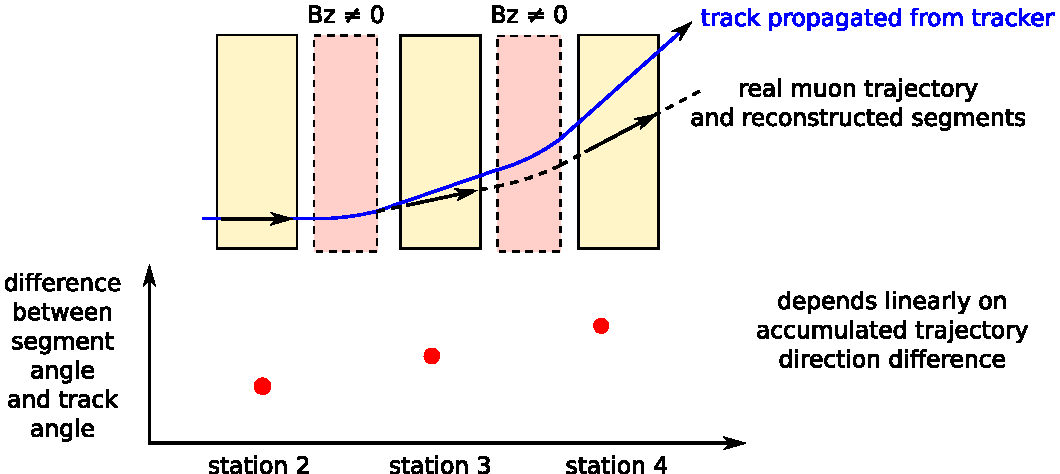
\includegraphics[width=\linewidth]{paths2.pdf}
\end{frame}

\begin{frame}
\frametitle{Reminder}

\begin{itemize}
\item Also possible to see the effect in {\it position} residuals
\item Deviation in position is an integral of the deviation in angle
\item More sensitive, but more difficult to interpret
\end{itemize}

\vfill
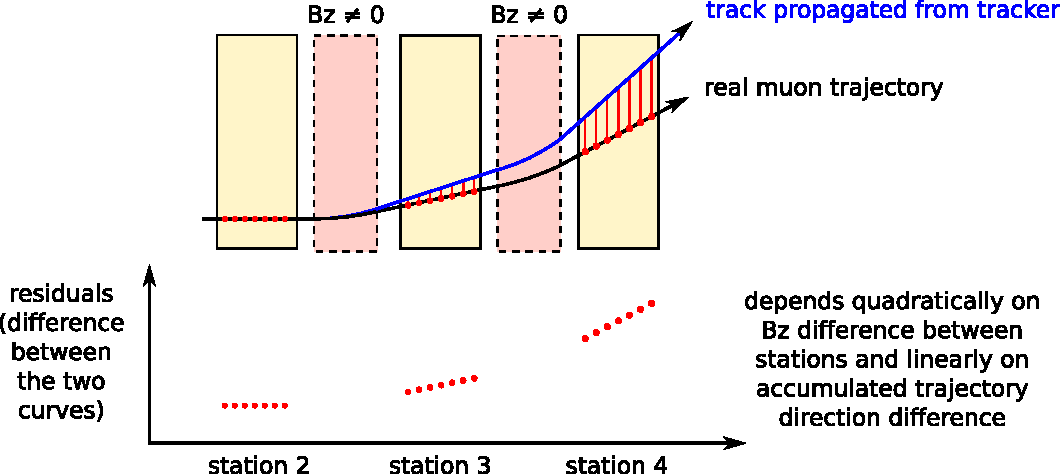
\includegraphics[width=\linewidth]{paths.pdf}
\end{frame}

\begin{frame}
\frametitle{Reminder}

\begin{itemize}
\item In either case, magnetic field affects positively and
  negatively-charged particles in opposite ways, while misalignment
  affects both equally
\item To be insensitive to any misalignment, we plot residuals from
  positively-charged tracks ($R_+$) minus residuals from
  negatively-charged tracks ($R_-$) over 2
\item This can't be performed on individual tracks: it must be binned into geographical regions
\item 1 region = 1/12$^{\mbox{\scriptsize th}}$ of a single chamber in $z$ (22~cm)
\end{itemize}

\begin{center}
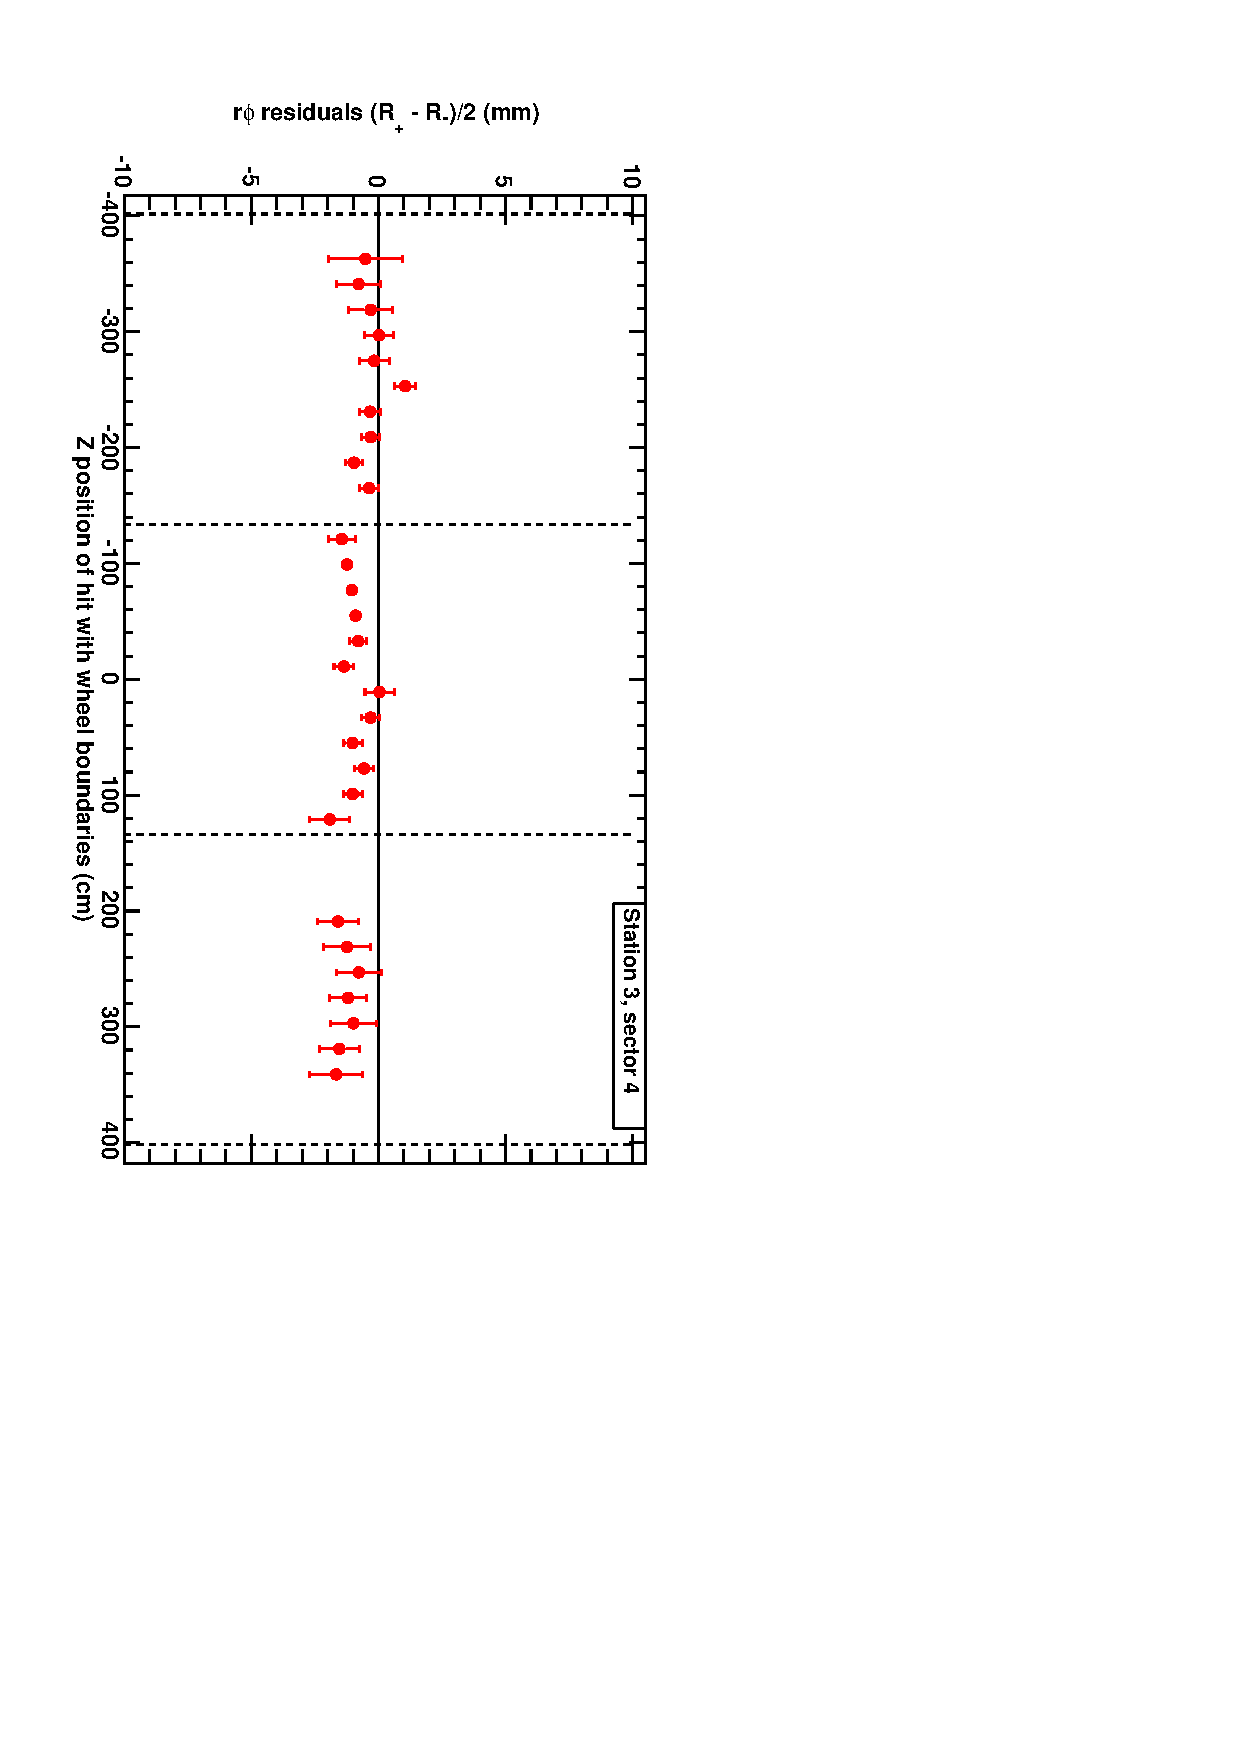
\includegraphics[height=0.75\linewidth, angle=90]{map40GeV_3_4.pdf}
\end{center}
\end{frame}

\begin{frame}
\frametitle{Results for $40 < p_T < 50$~GeV}

\begin{columns}
\column{0.7\linewidth}
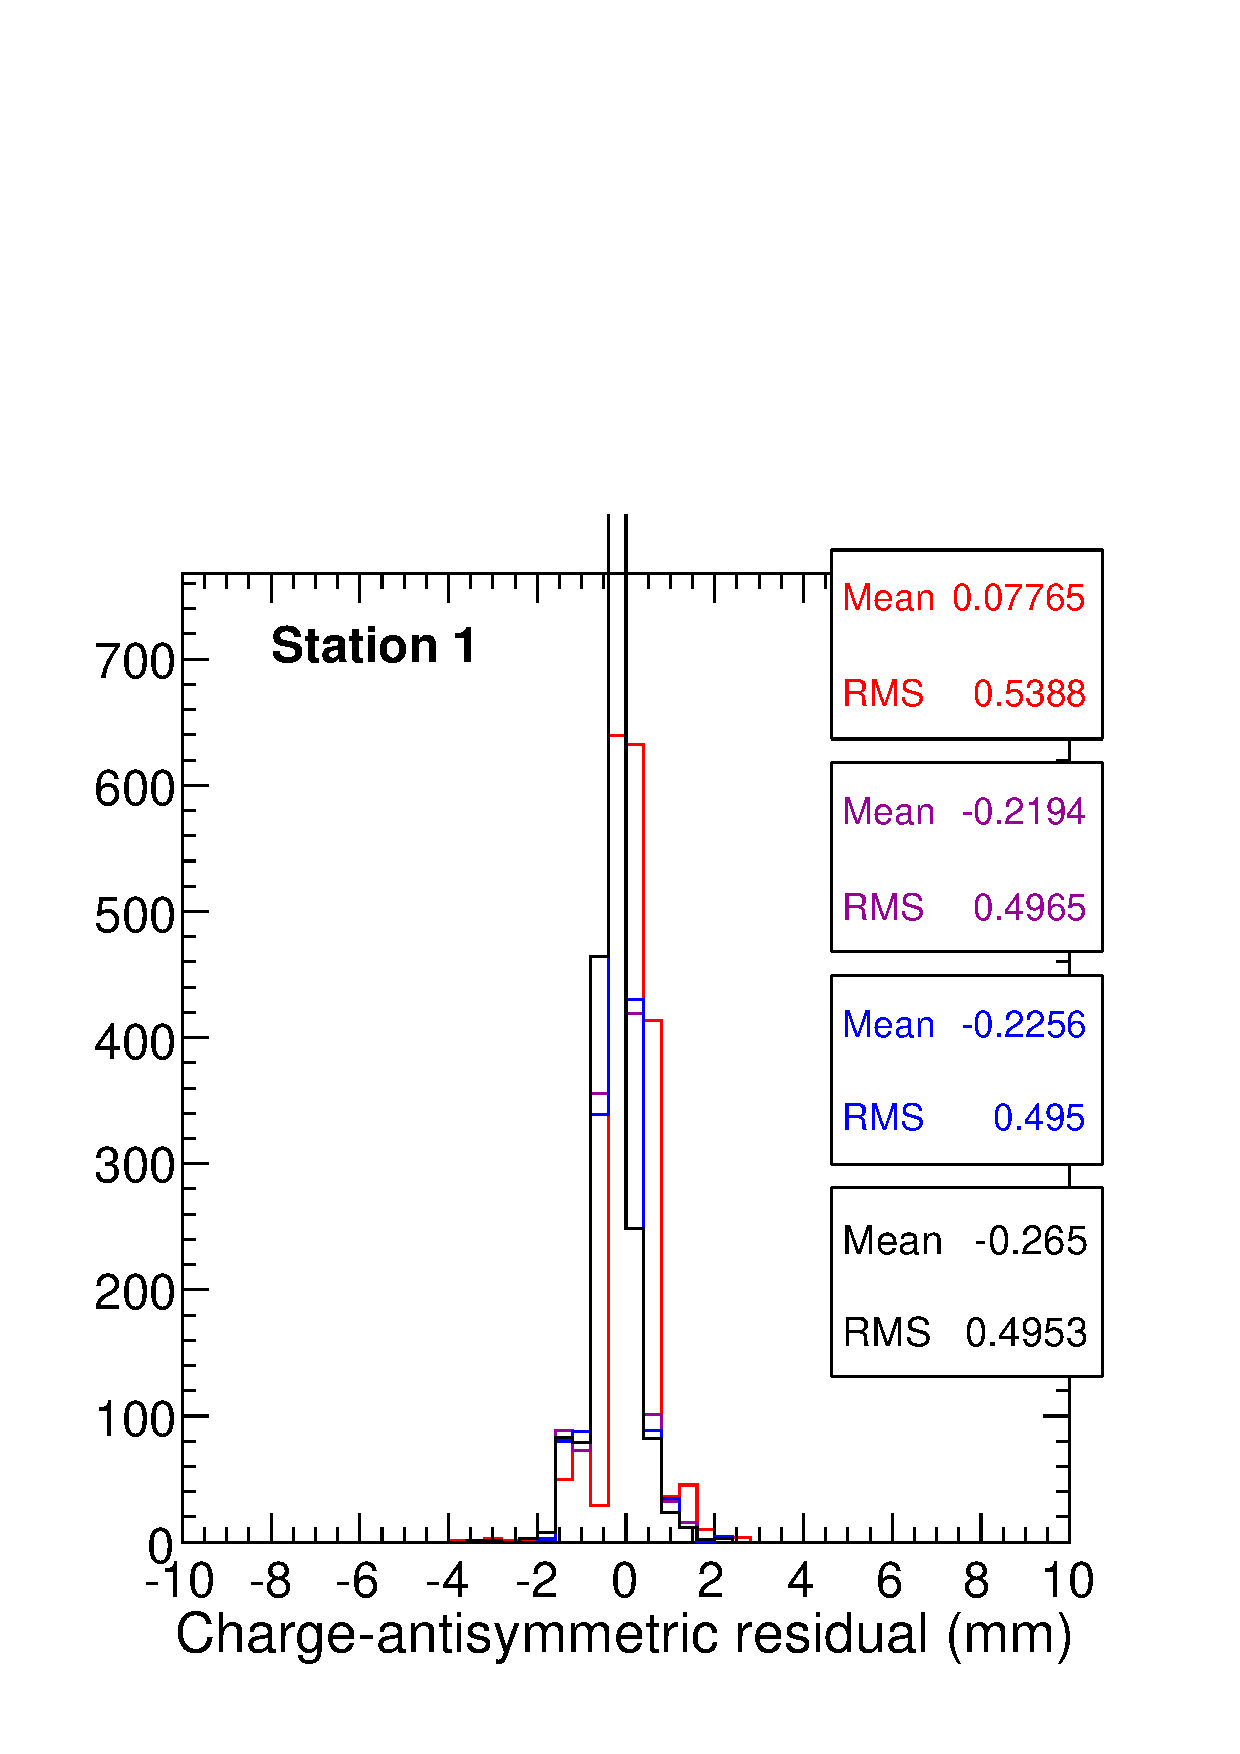
\includegraphics[width=0.5\linewidth]{station1_ptcut40.pdf}
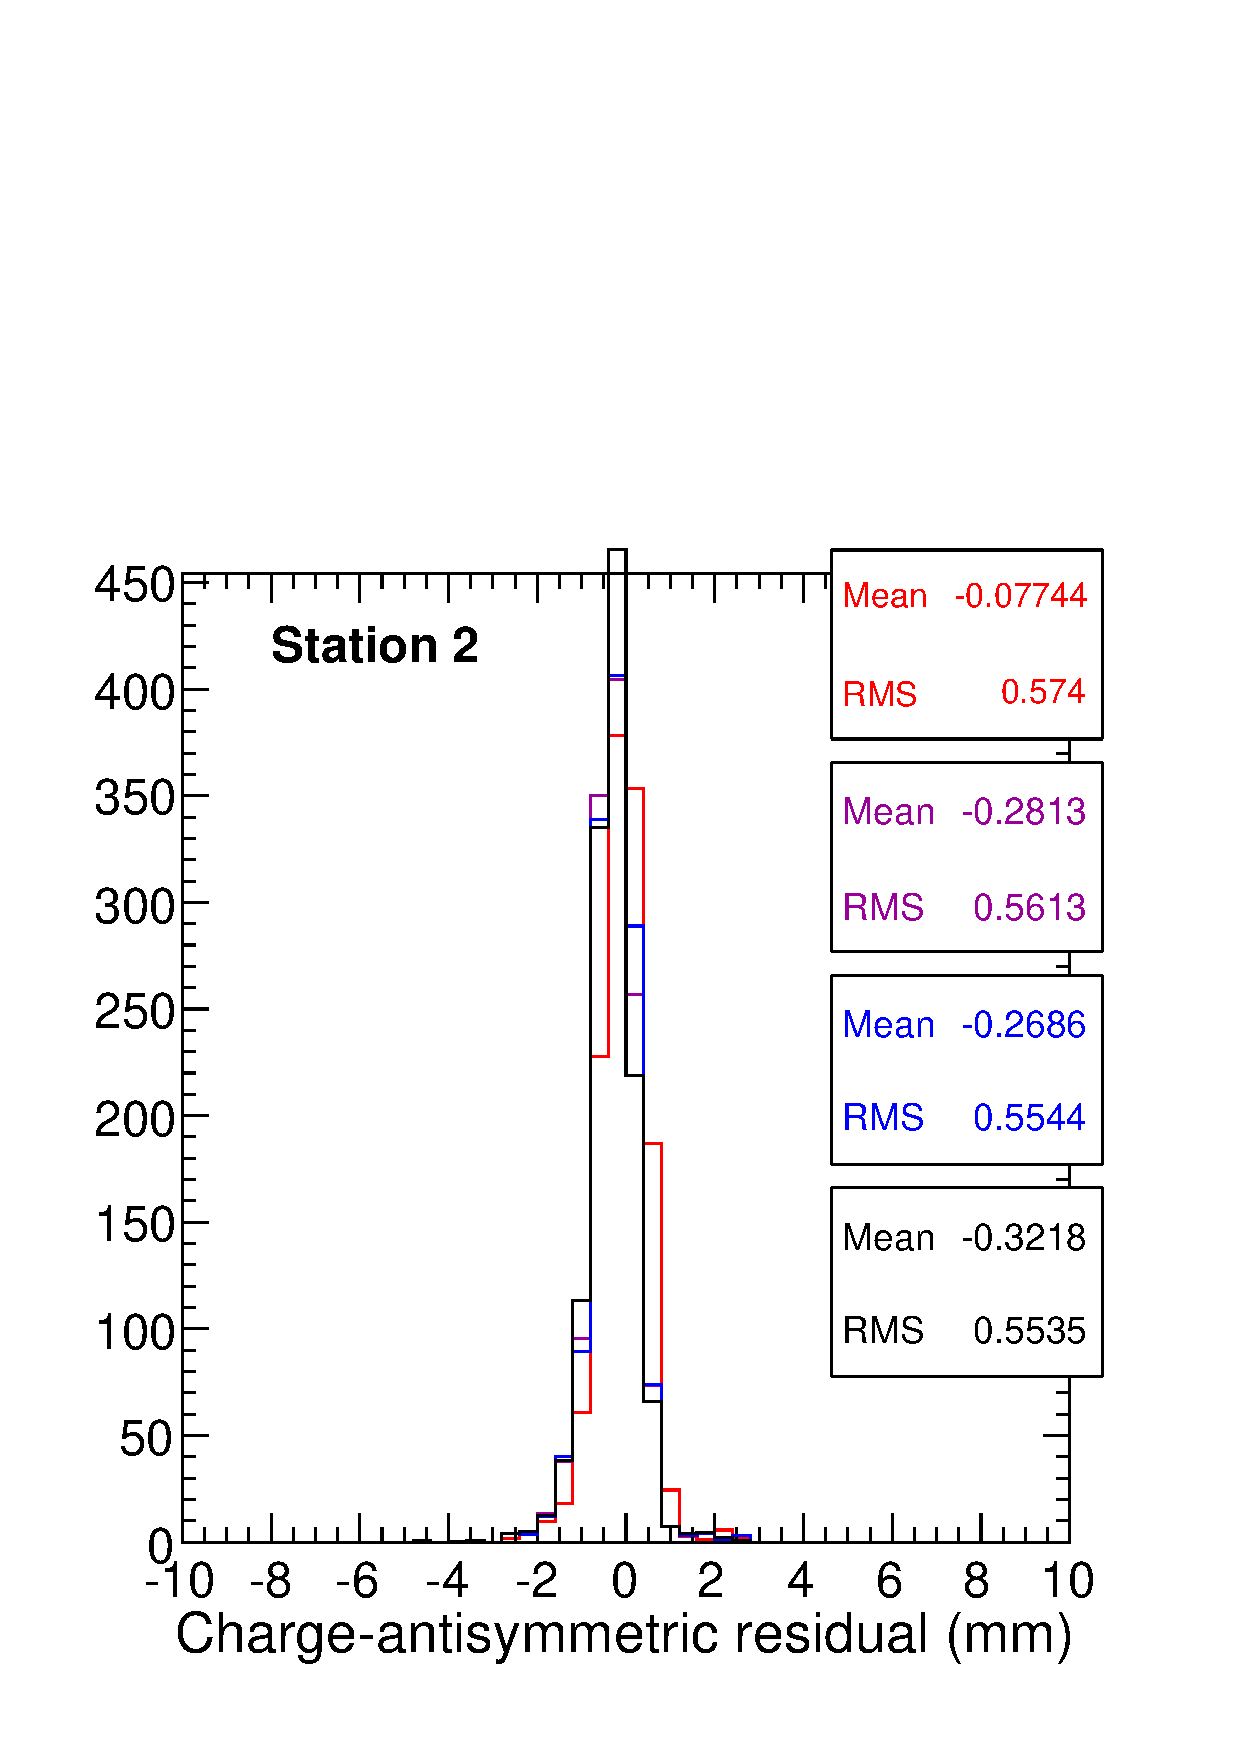
\includegraphics[width=0.5\linewidth]{station2_ptcut40.pdf}

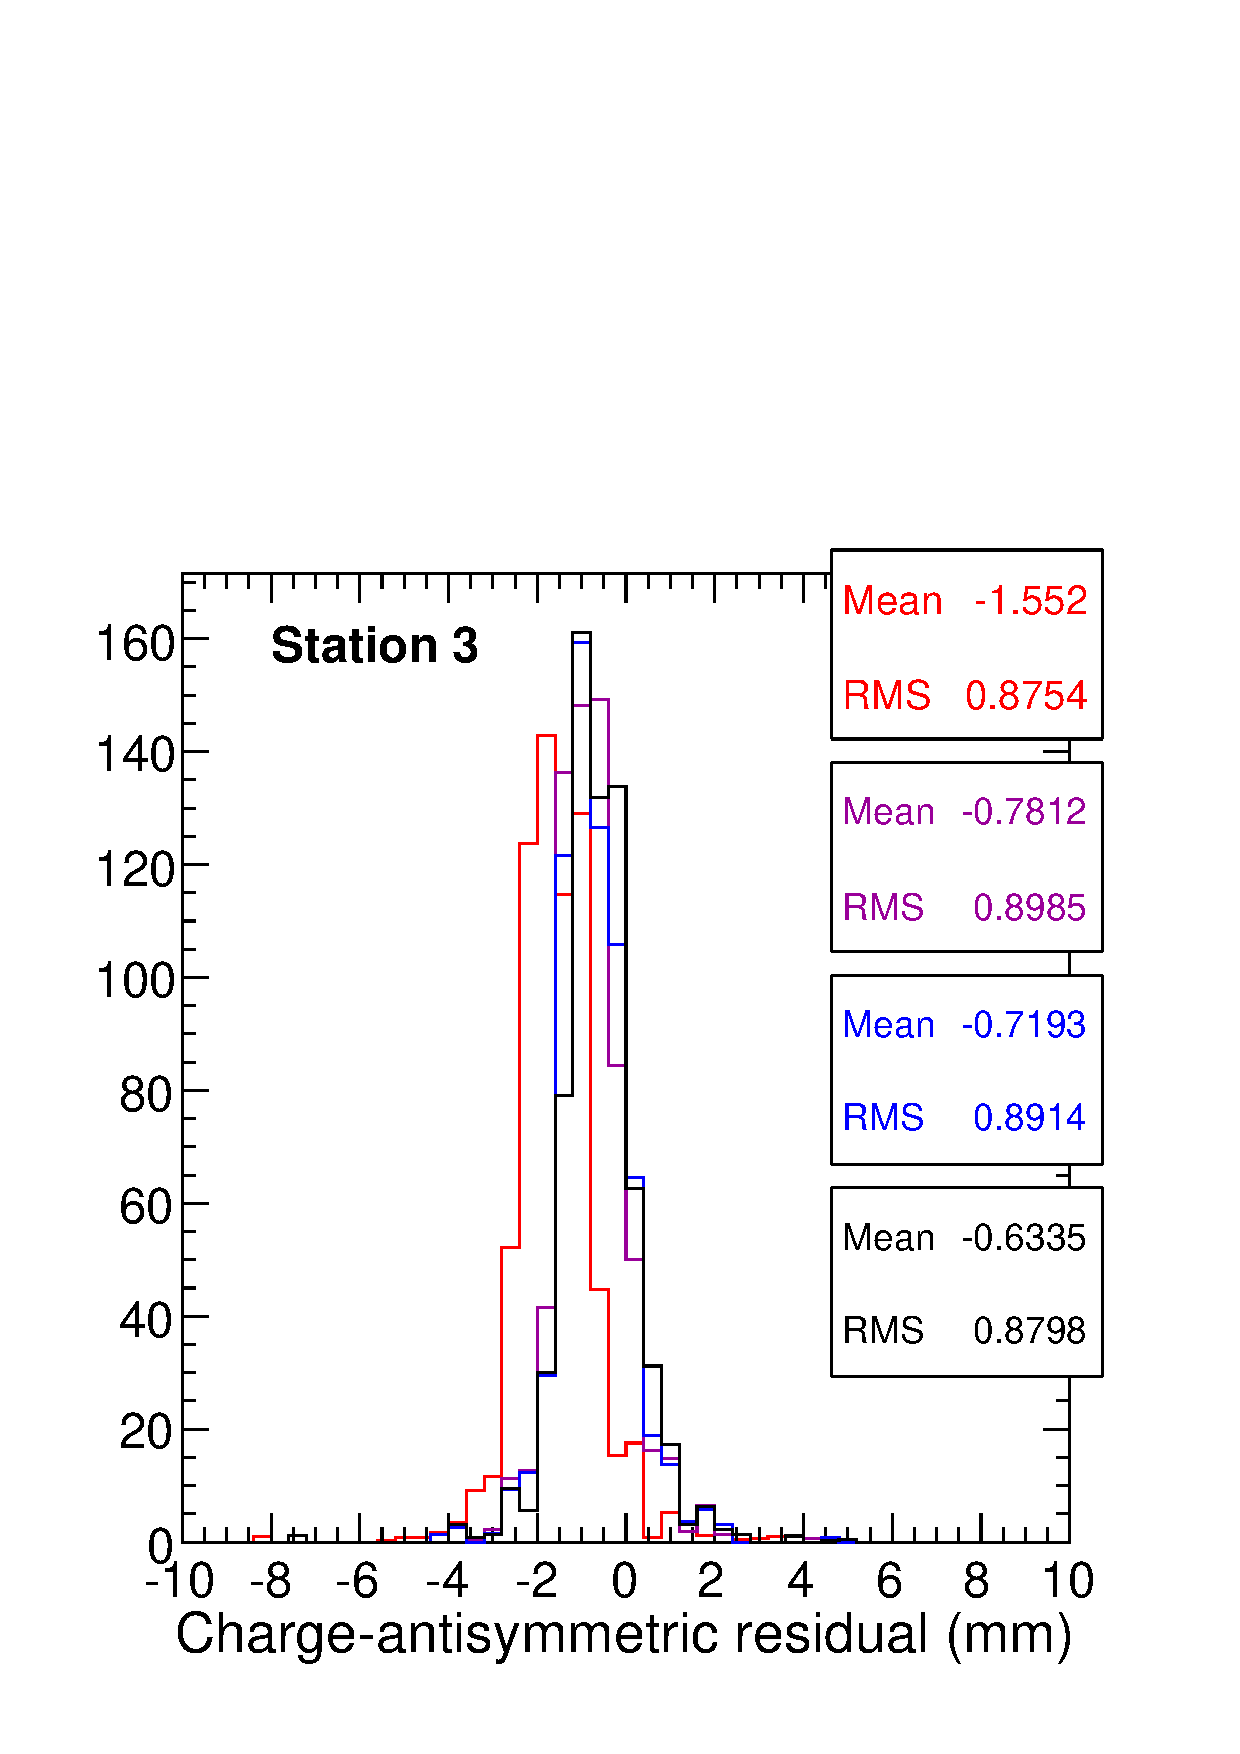
\includegraphics[width=0.5\linewidth]{station3_ptcut40.pdf}
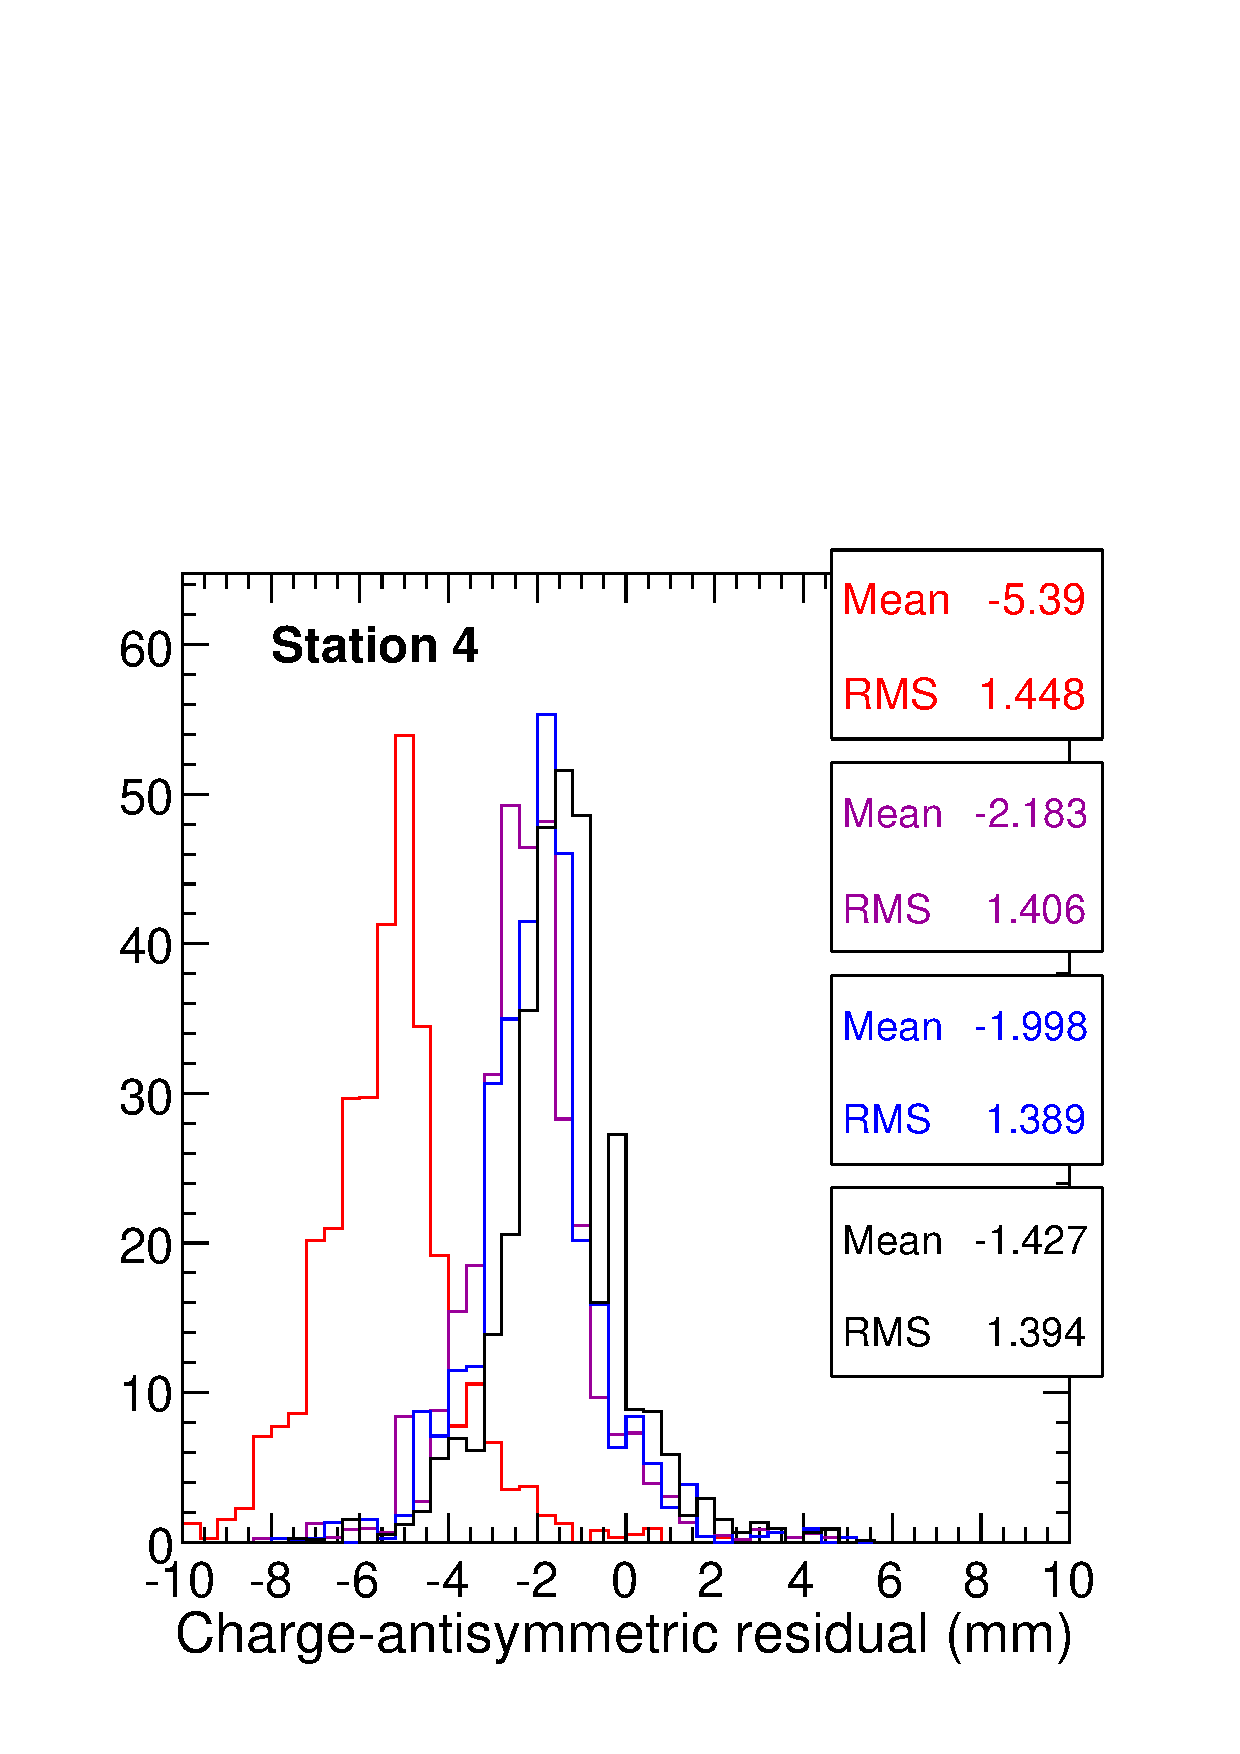
\includegraphics[width=0.5\linewidth]{station4_ptcut40.pdf}

\column{0.3\linewidth}
\scriptsize
\begin{itemize}
\item Histograms of charge differences (one entry per ``geographical region'')
\item Color code:

\textcolor{red}{red: original map}

\textcolor{purple}{purple: radius $\to$ 30~m}

\textcolor{blue}{blue: radius and $|z|$ $\to$ 30~m}

\textcolor{black}{black: with scaling factors, for 3\_1\_X}

\item Final map is not perfectly centered
\end{itemize}

\vspace{0.5 cm}
\tiny (Calculation includes latest tracker, muon alignment, and CMSSW version)
\end{columns}
\end{frame}

\begin{frame}
\frametitle{Individual bins vs.~$z$}
\framesubtitle{Station 3 (positive $-$ negative)/2 versus $z$}

2.~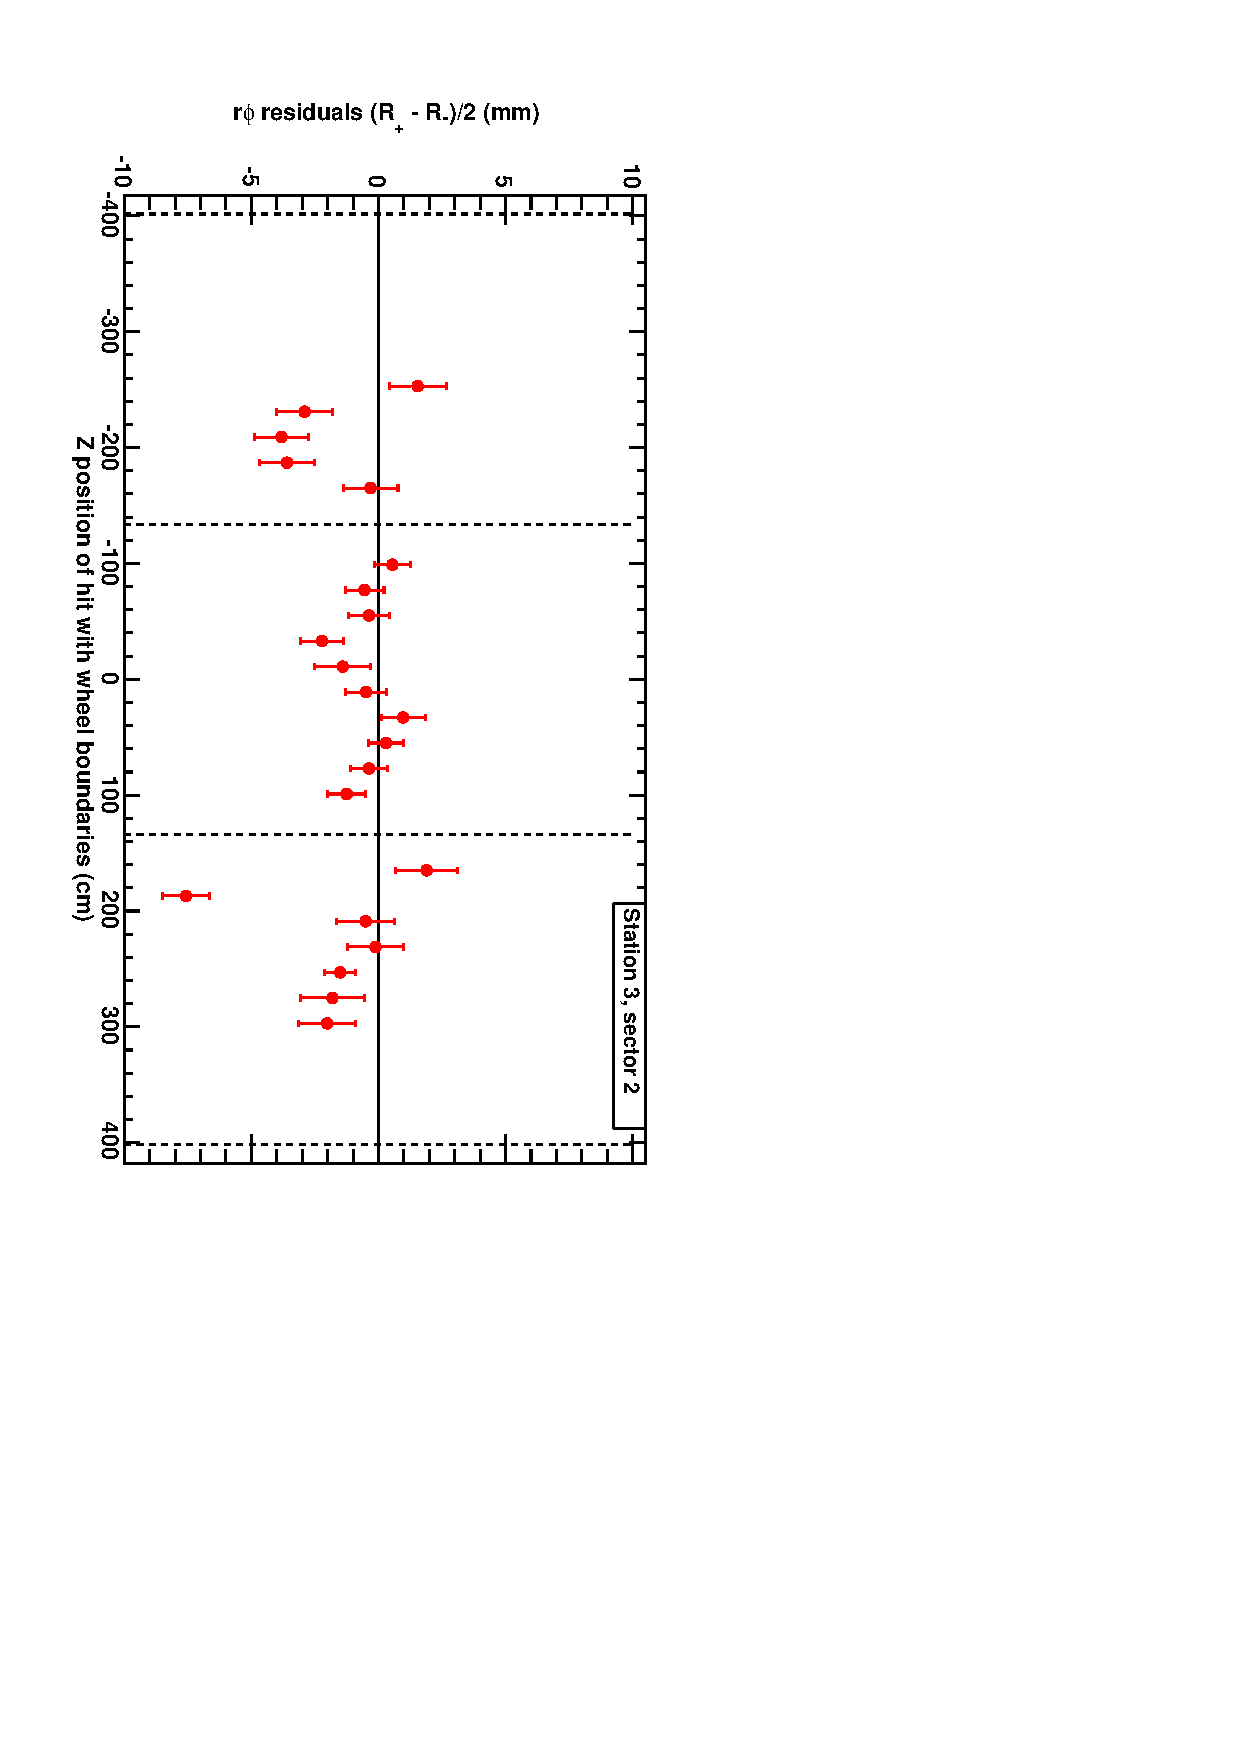
\includegraphics[height=0.28\linewidth, angle=90]{map40GeV_3_2.pdf} \hfill
3.~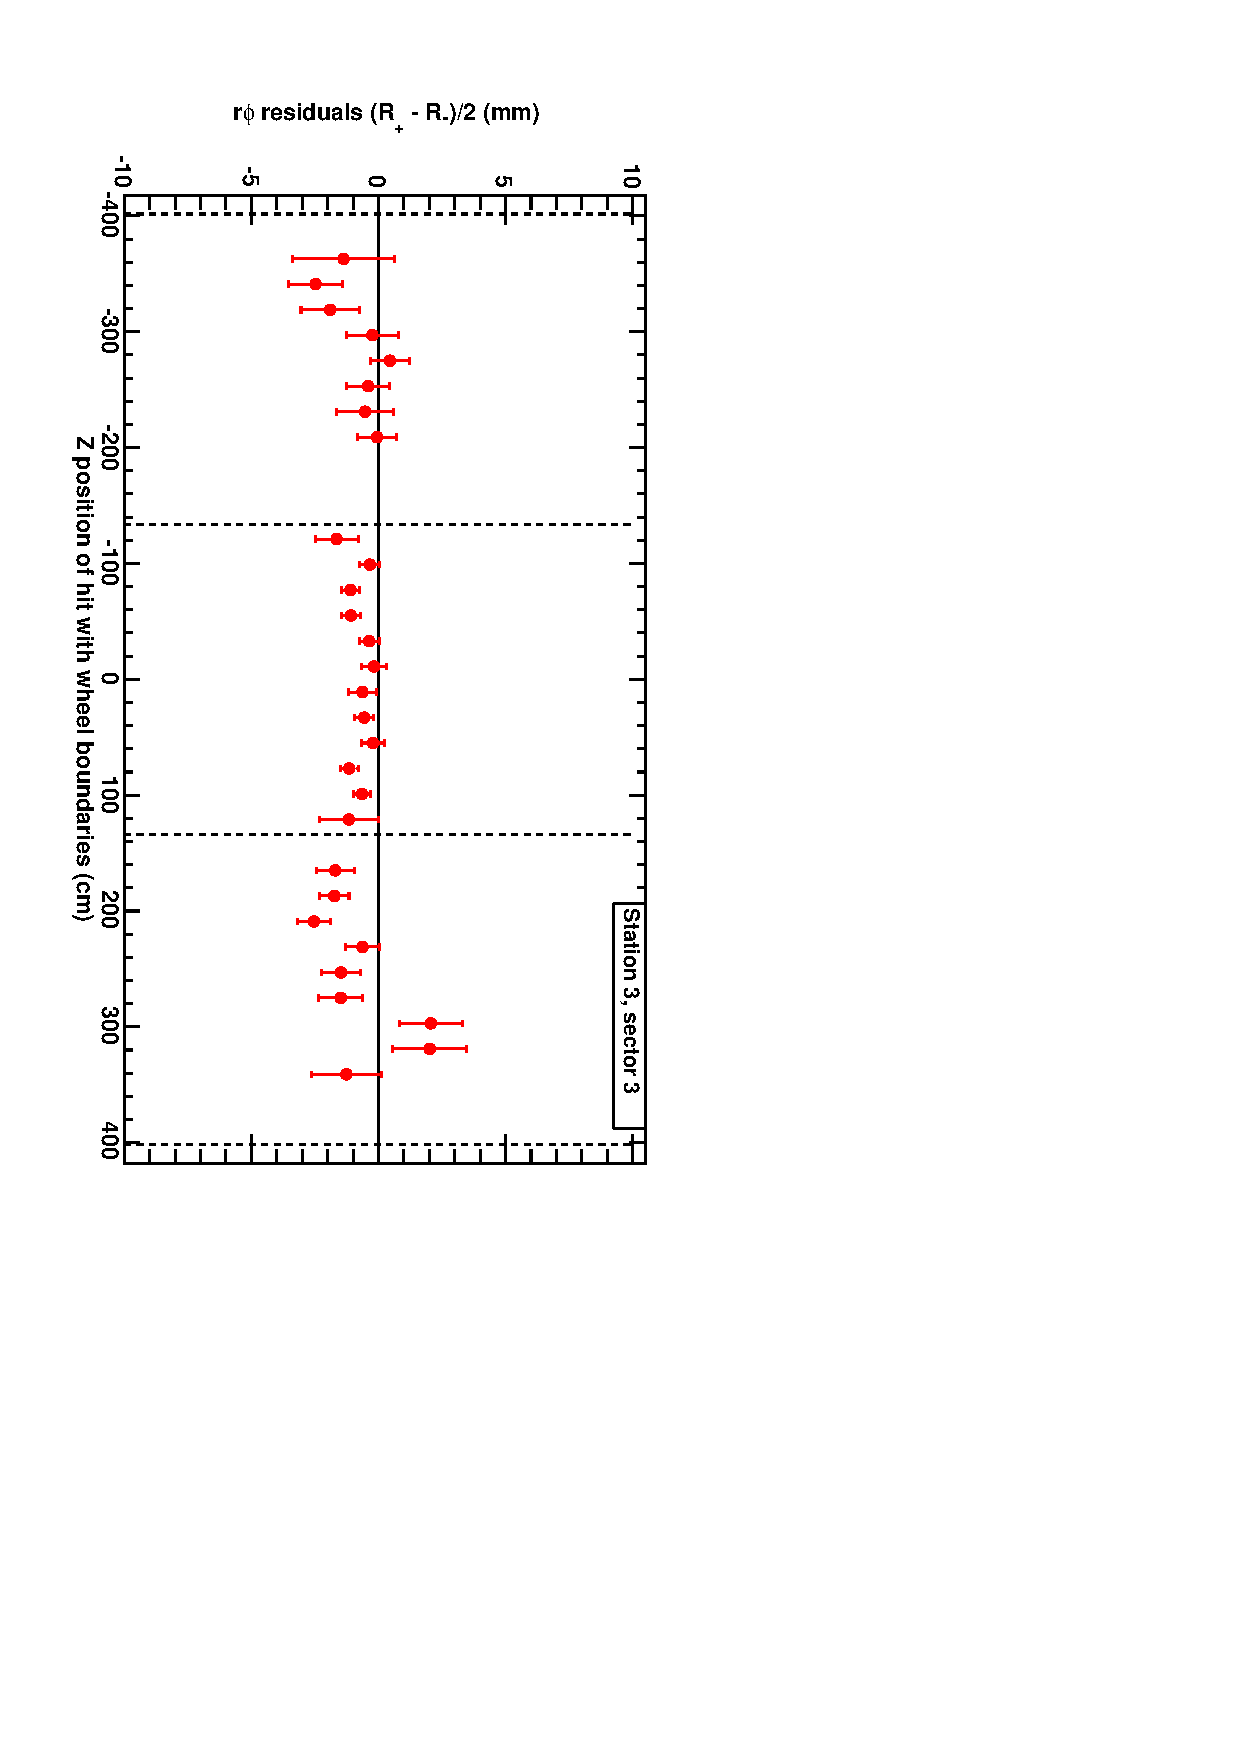
\includegraphics[height=0.28\linewidth, angle=90]{map40GeV_3_3.pdf} \hfill
4.~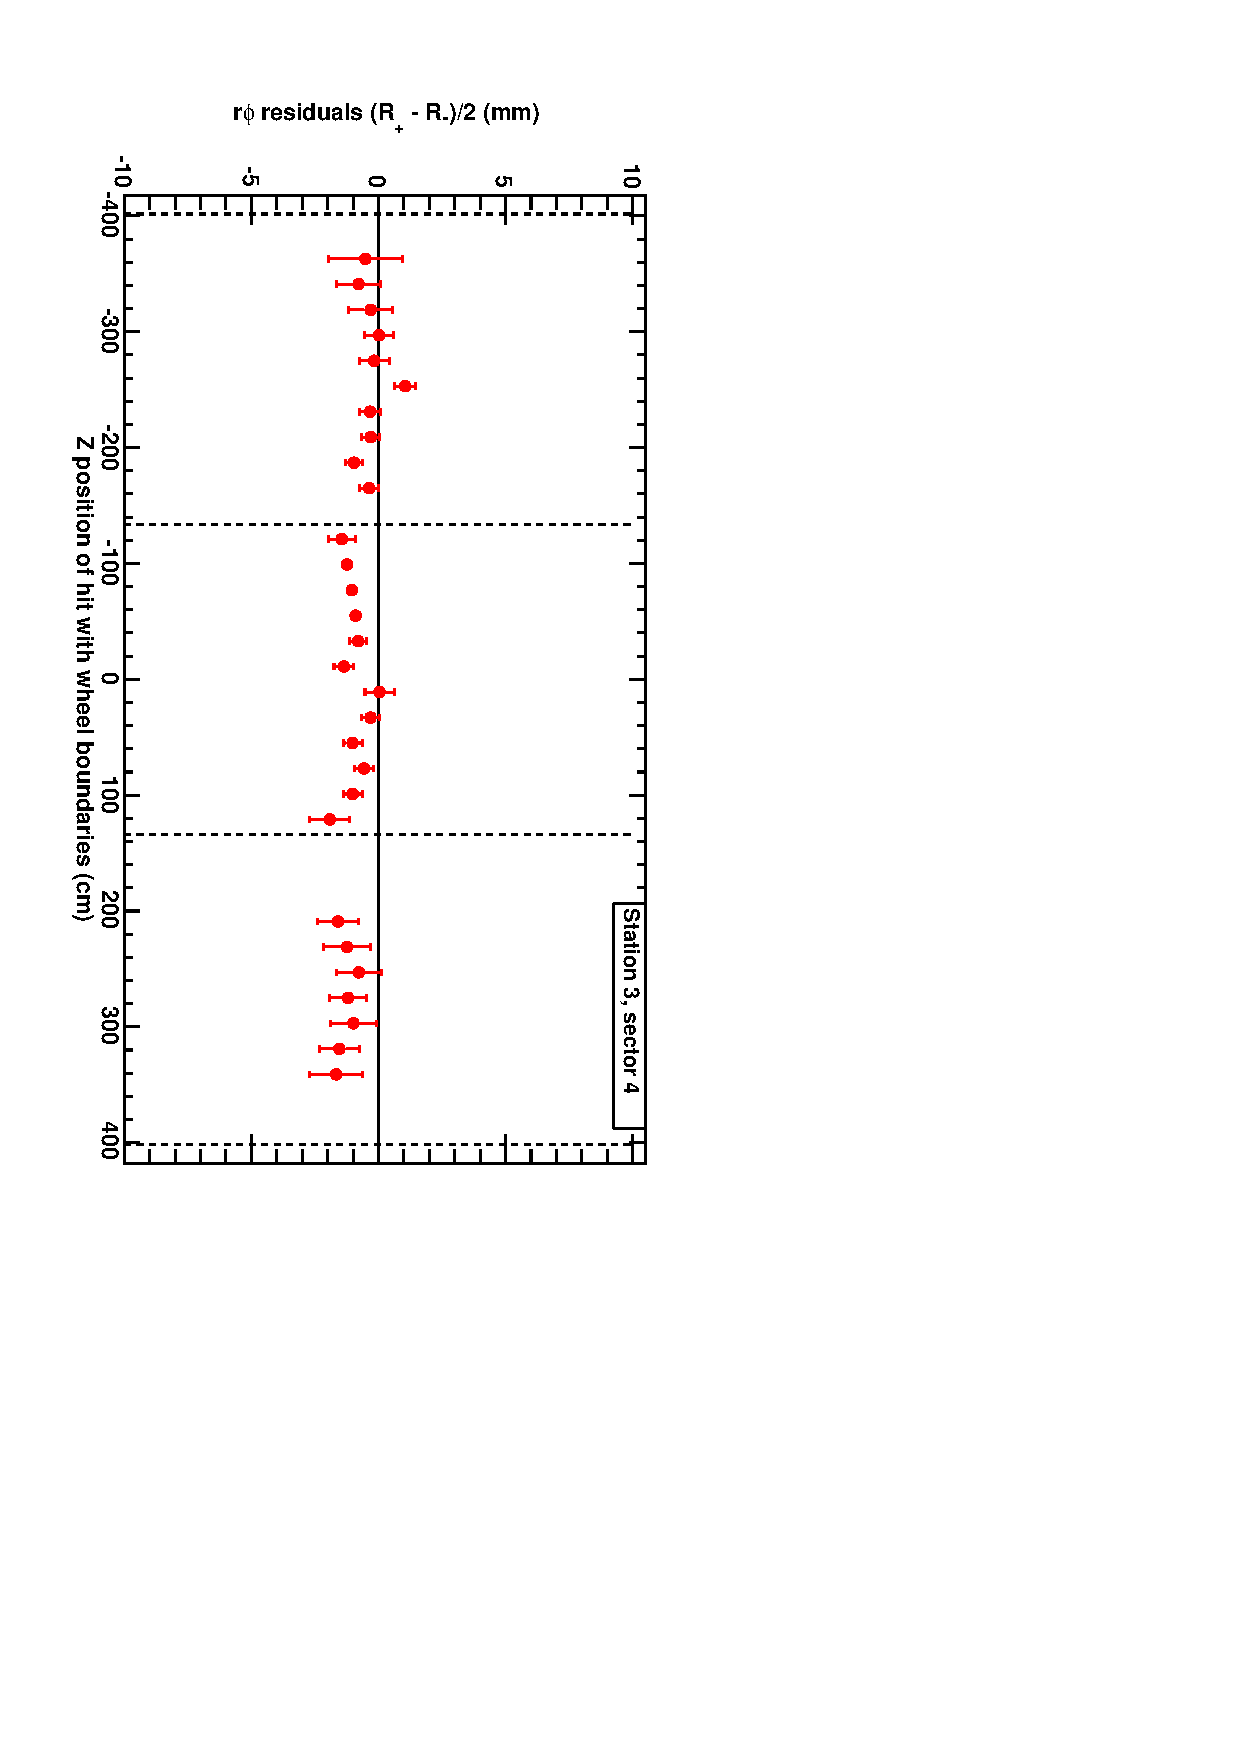
\includegraphics[height=0.28\linewidth, angle=90]{map40GeV_3_4.pdf}

\vspace{0.3 cm}
5.~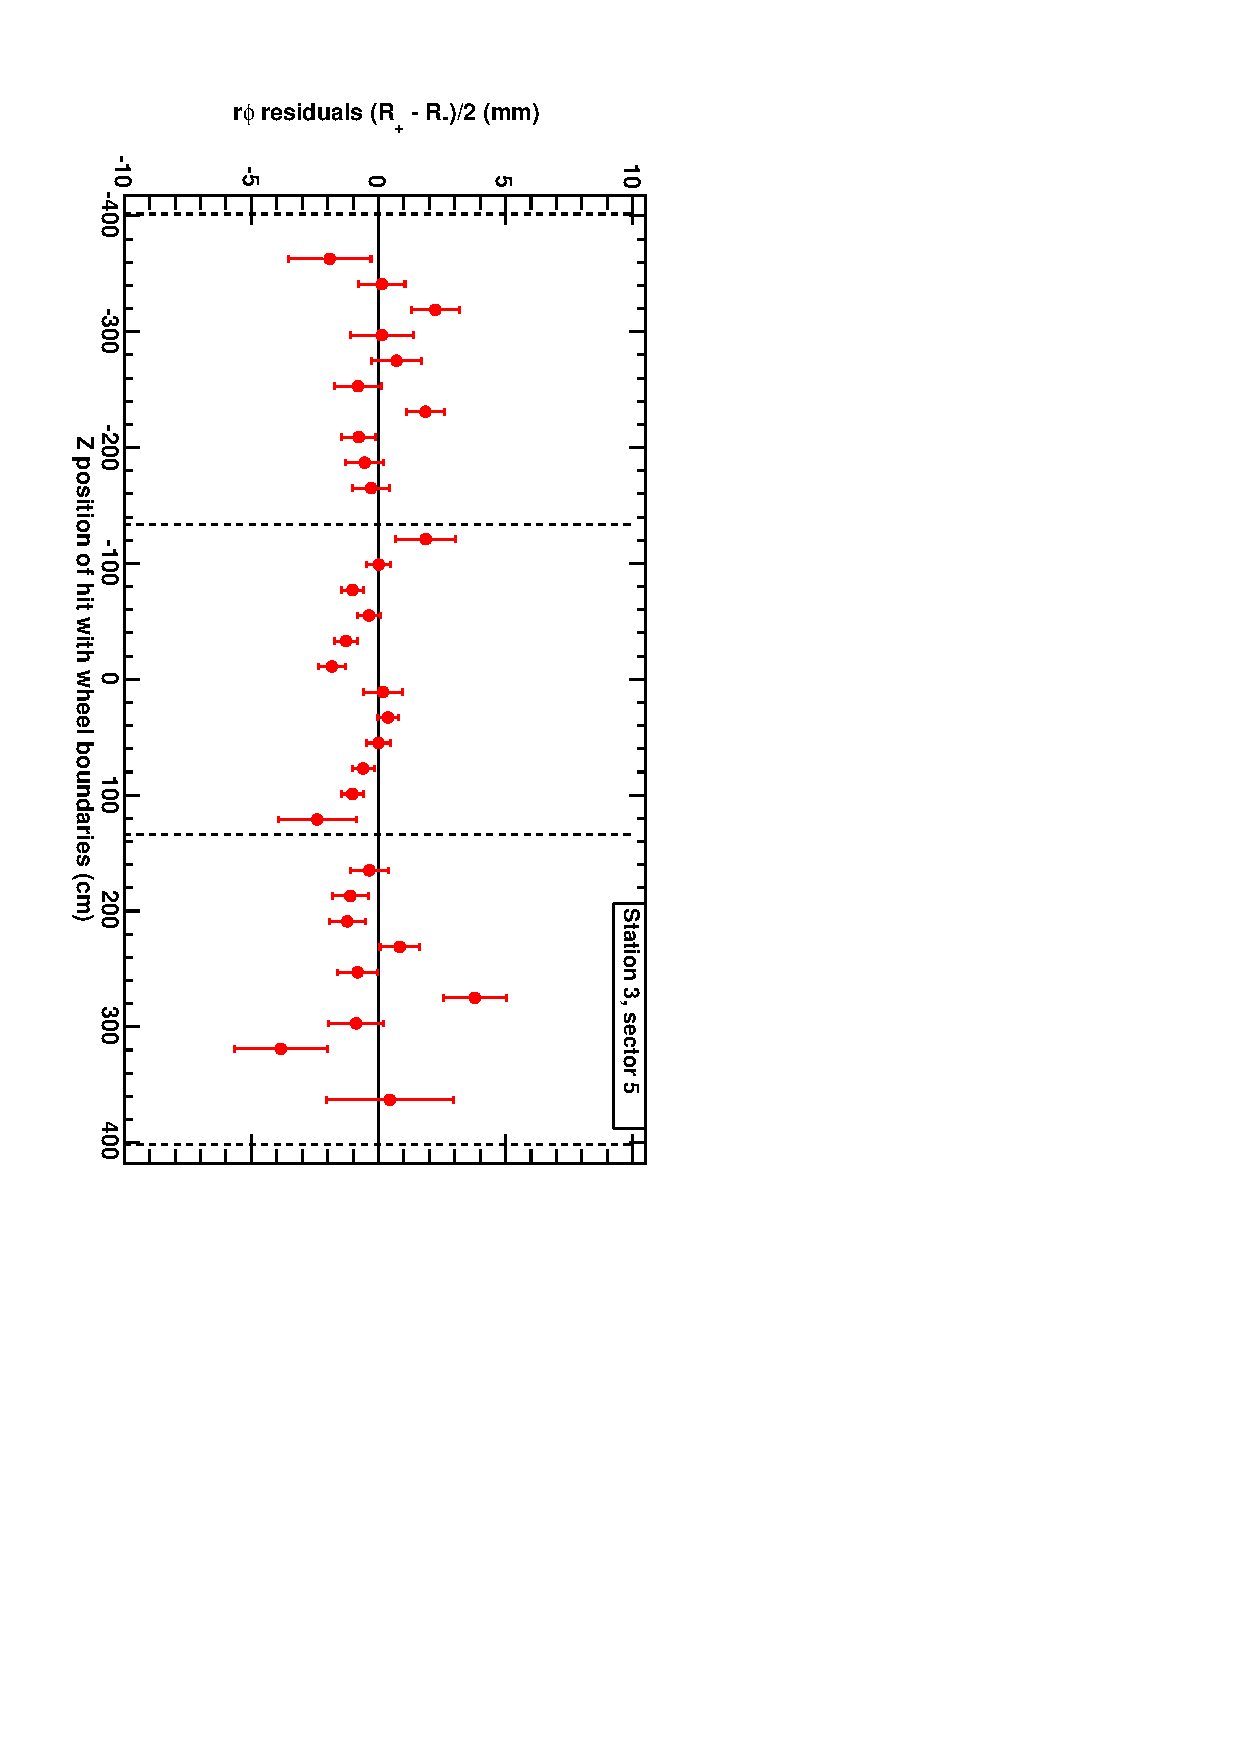
\includegraphics[height=0.28\linewidth, angle=90]{map40GeV_3_5.pdf} \hfill
6.~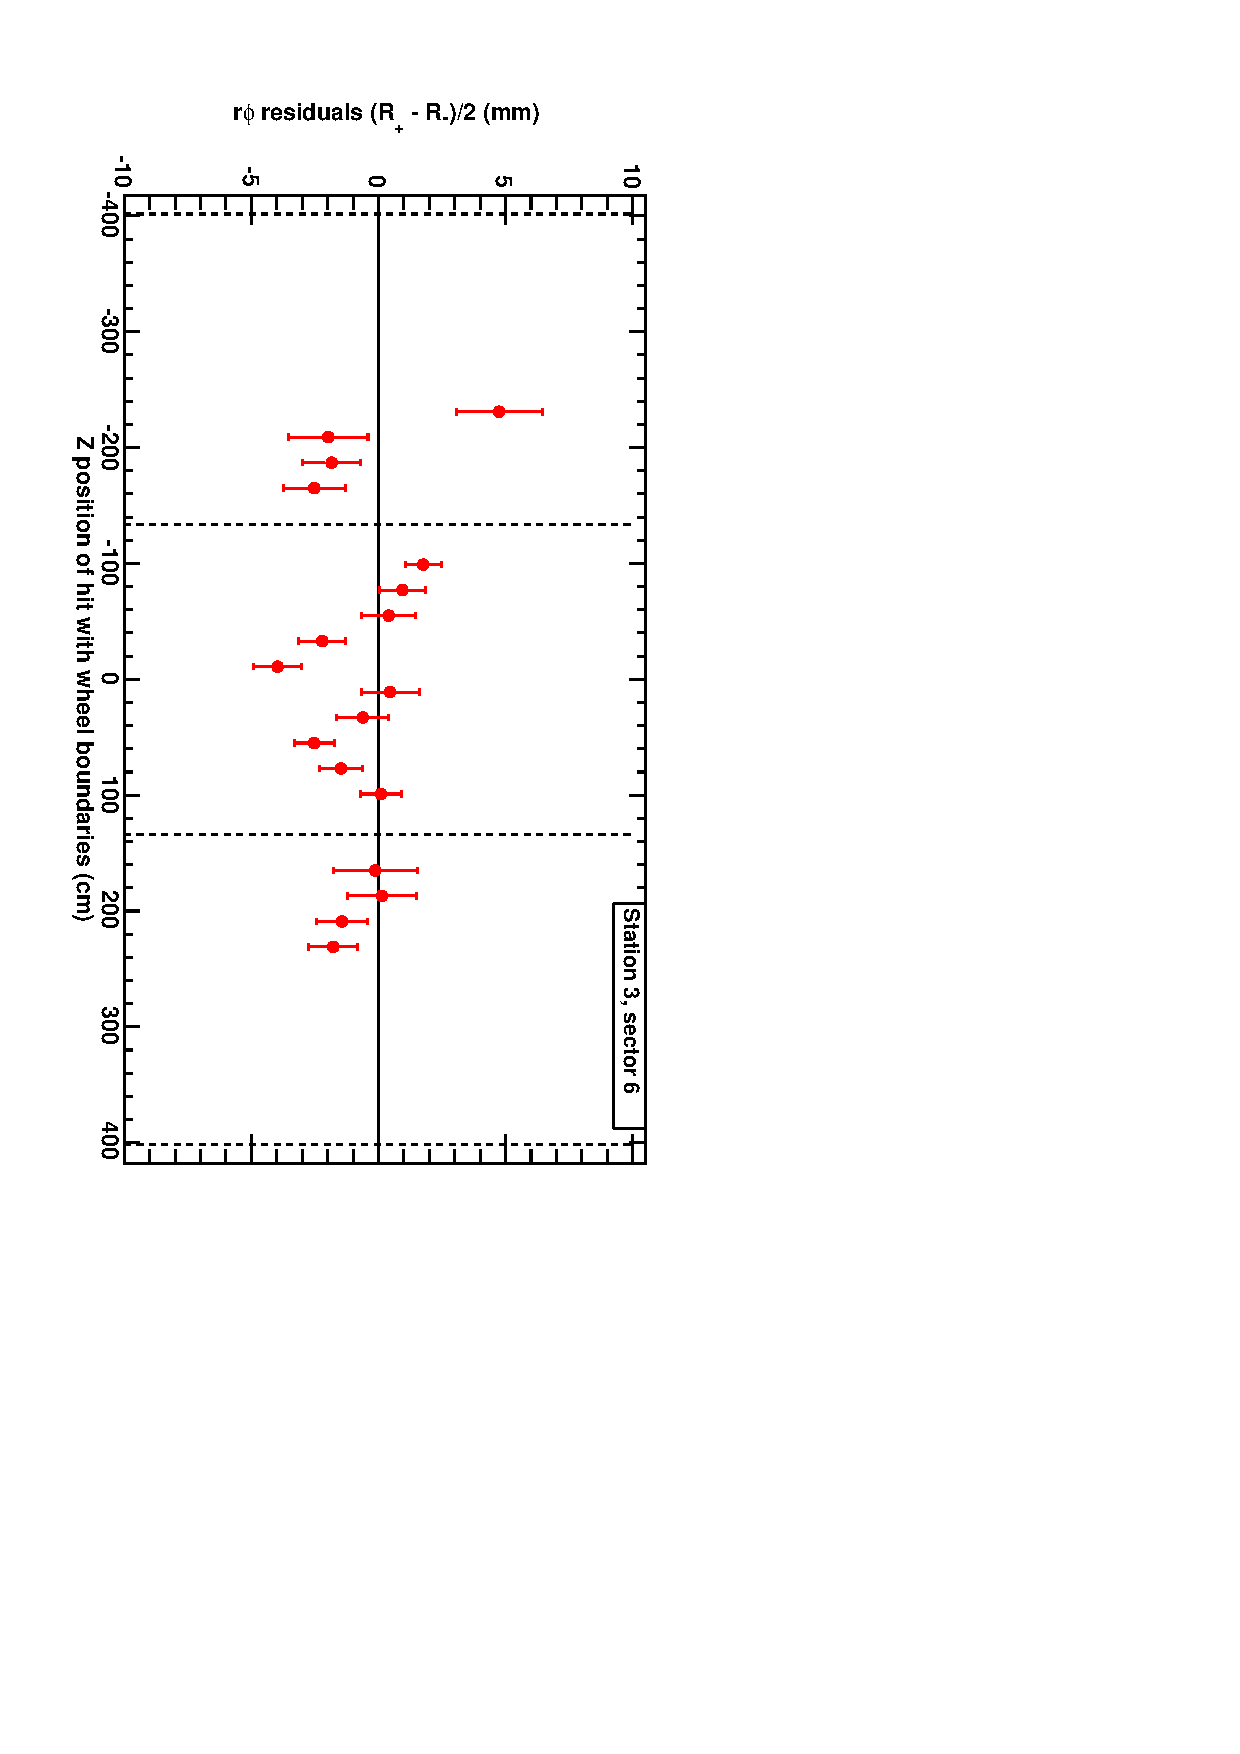
\includegraphics[height=0.28\linewidth, angle=90]{map40GeV_3_6.pdf} \hfill
8.~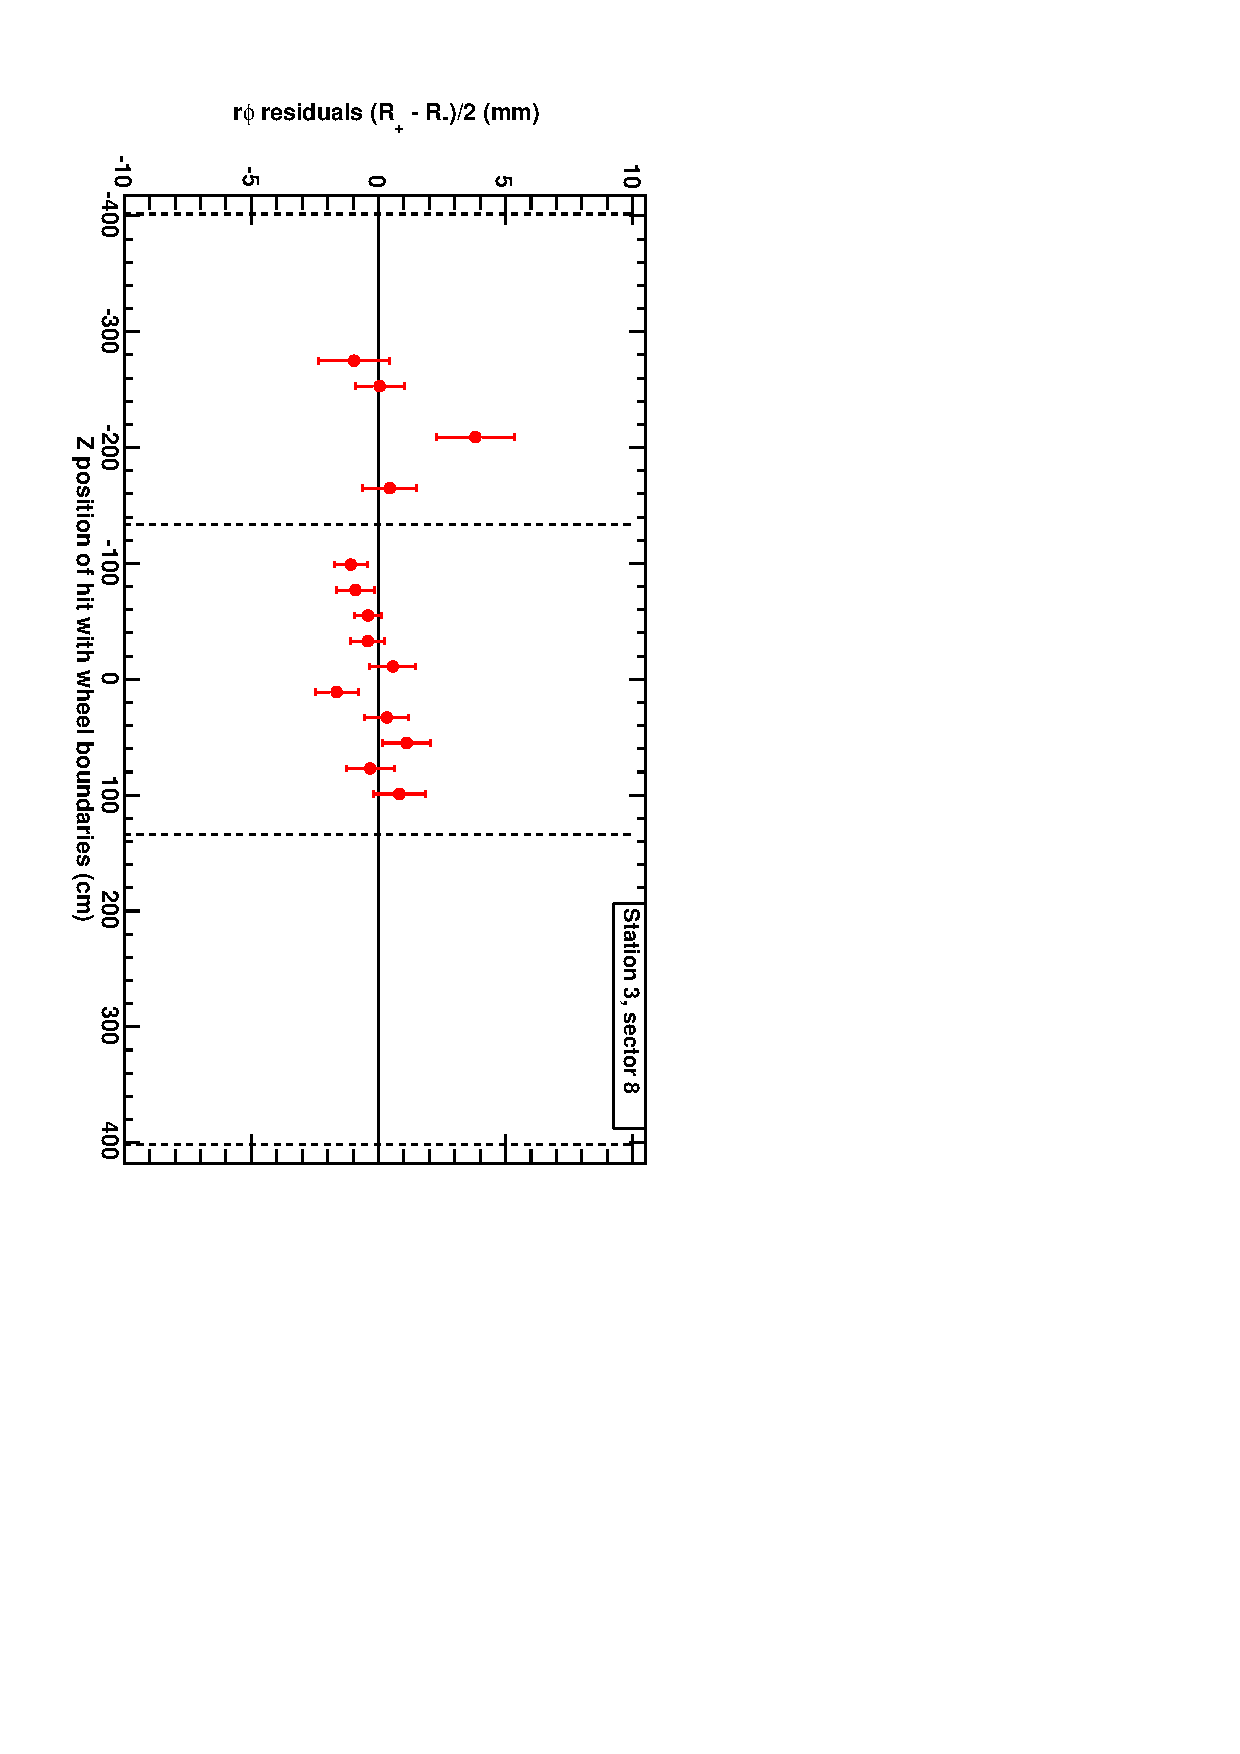
\includegraphics[height=0.28\linewidth, angle=90]{map40GeV_3_8.pdf}

\vspace{0.3 cm}
9.~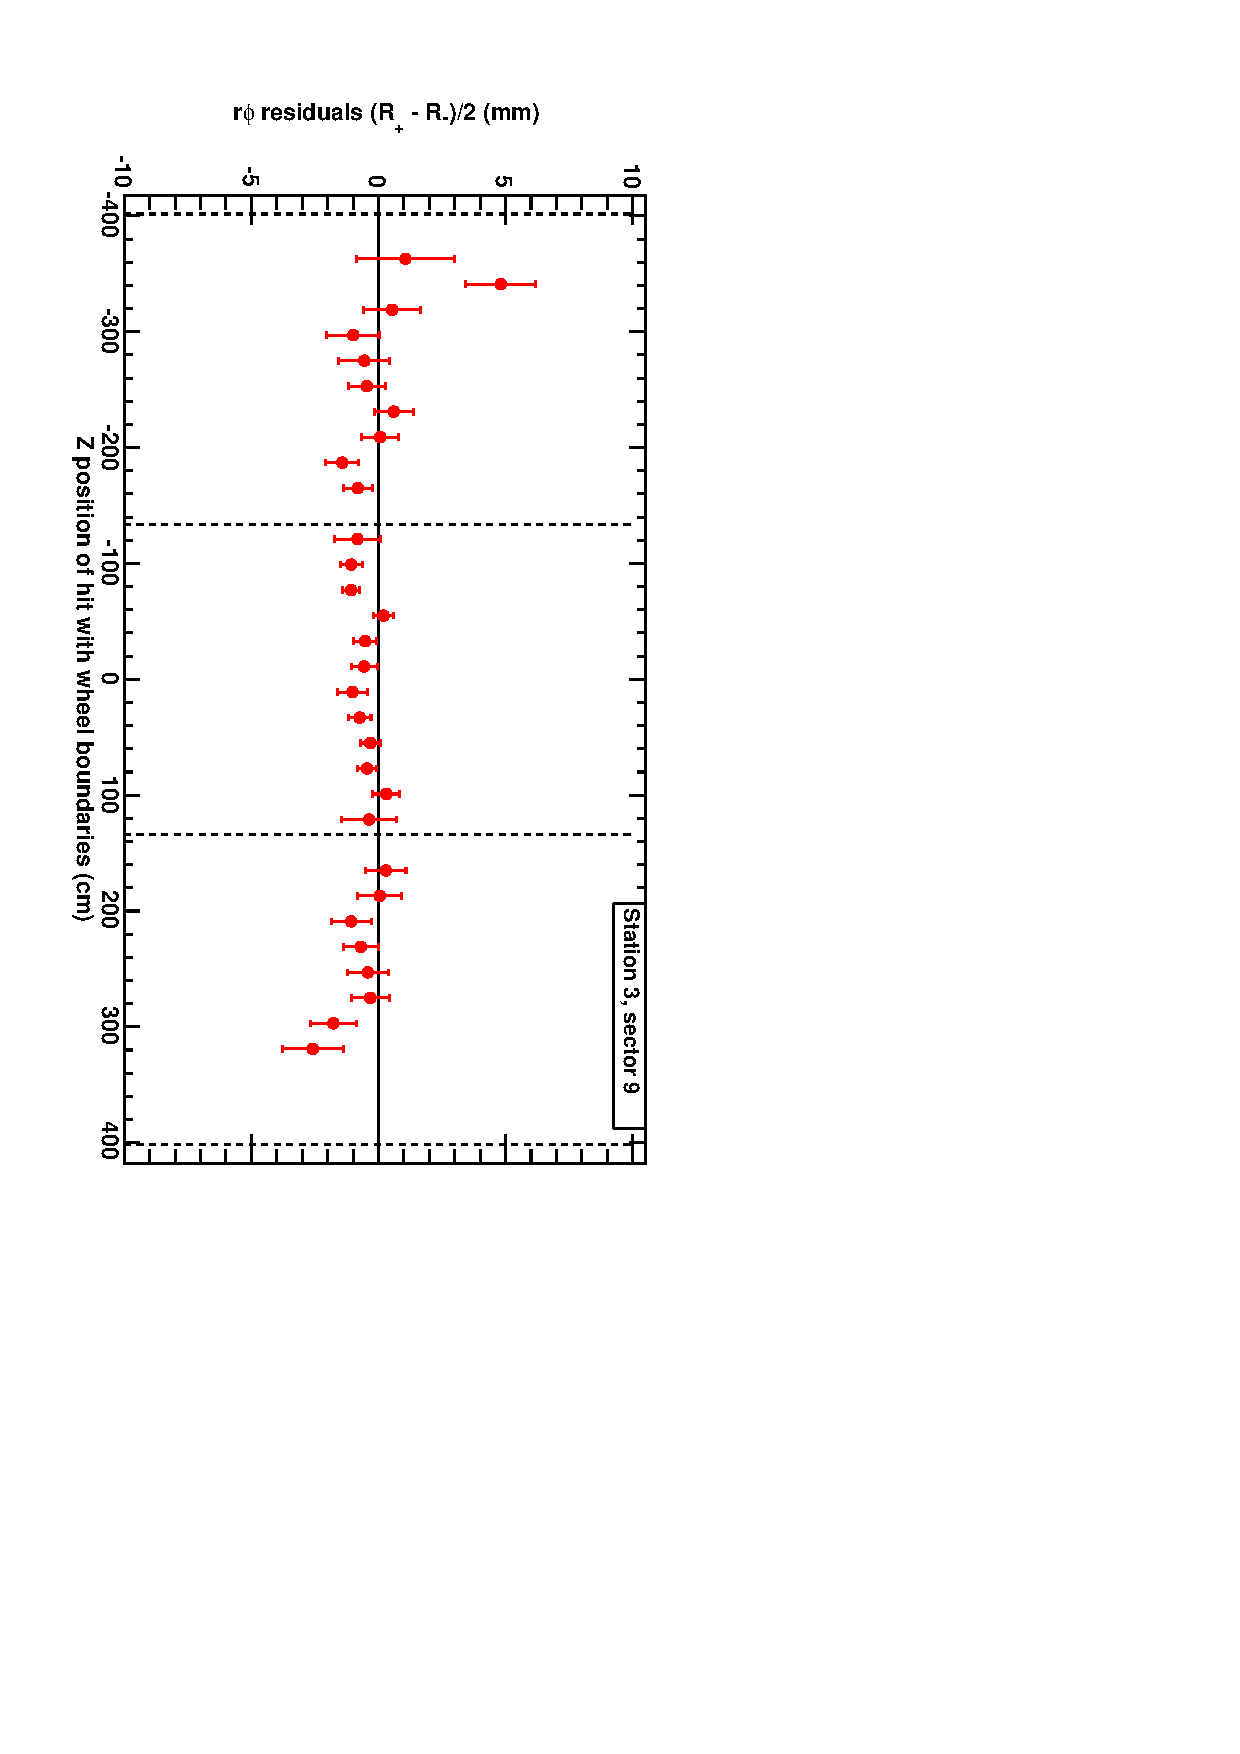
\includegraphics[height=0.28\linewidth, angle=90]{map40GeV_3_9.pdf} \hfill
10.~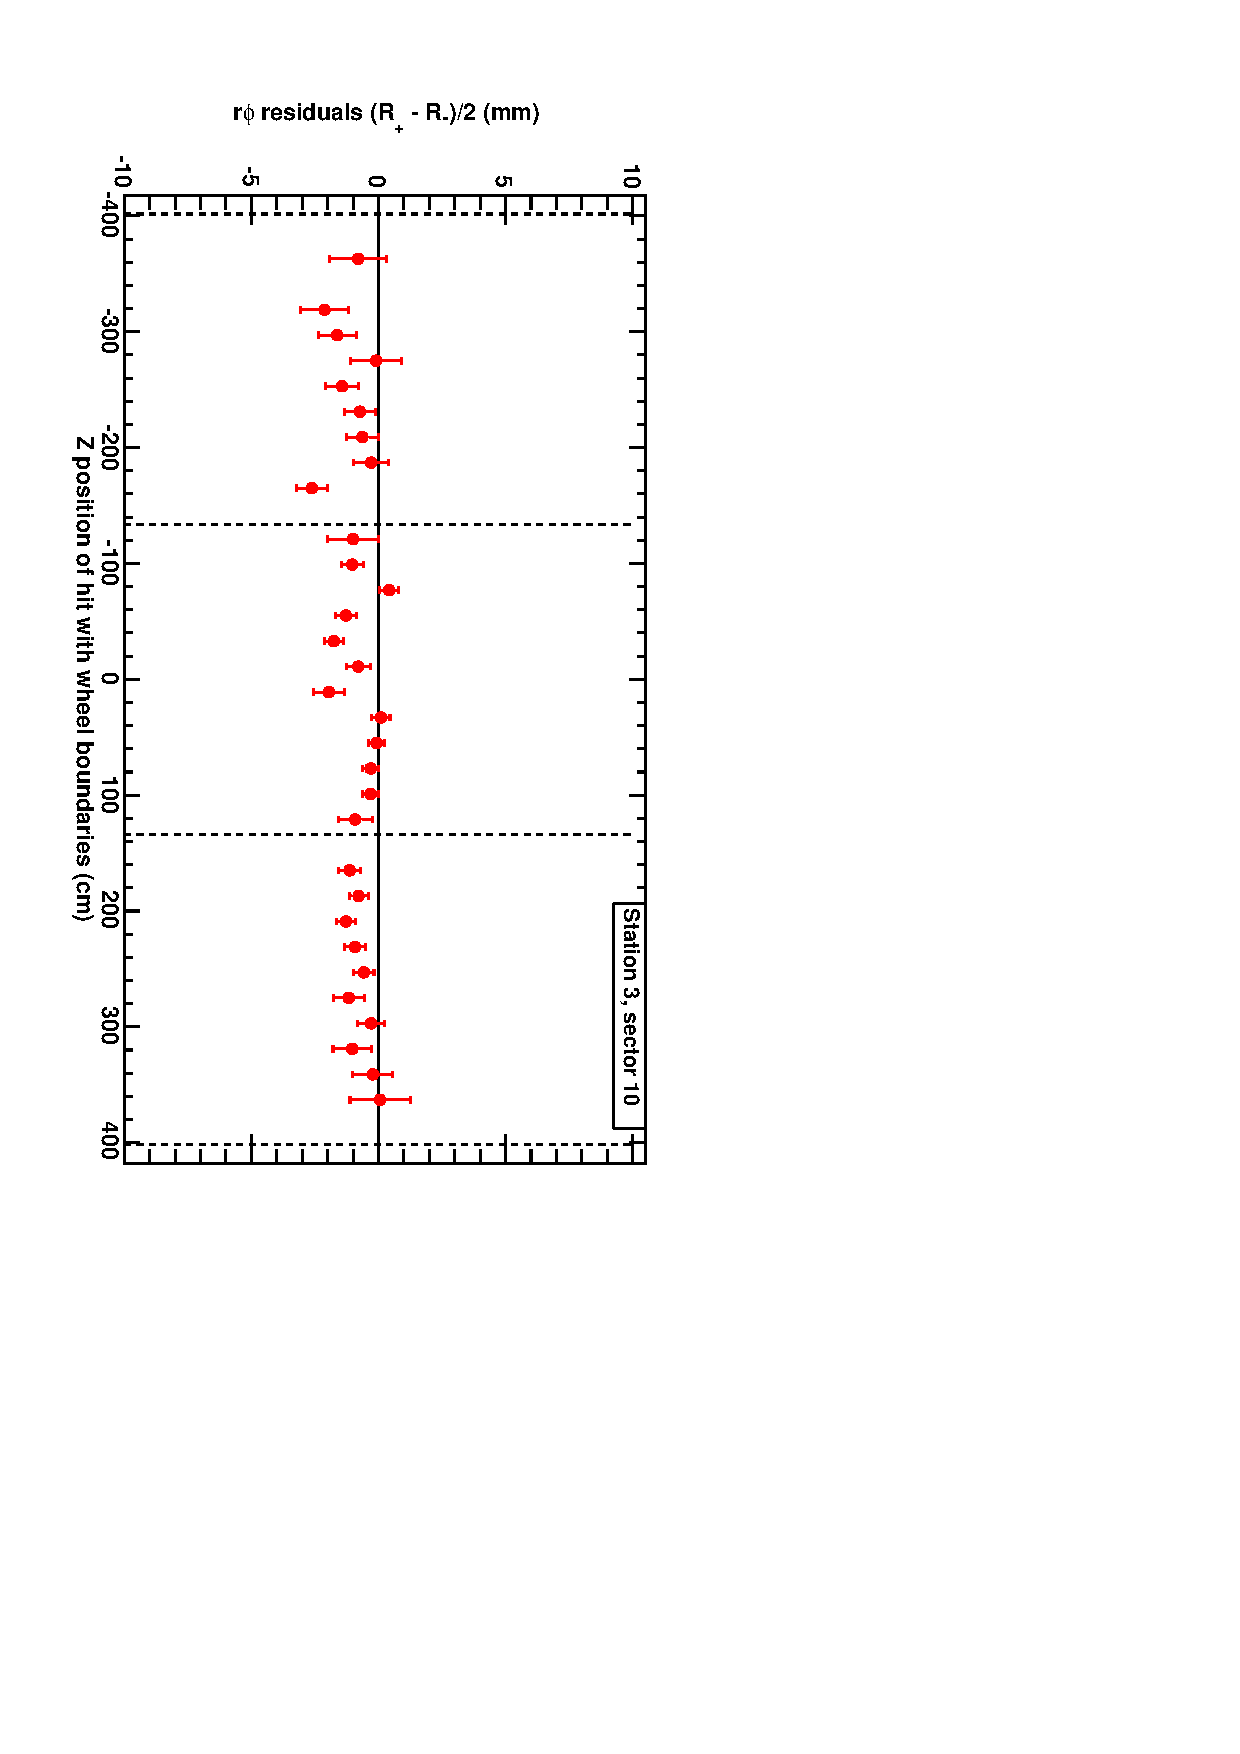
\includegraphics[height=0.28\linewidth, angle=90]{map40GeV_3_10.pdf} \hfill
11.~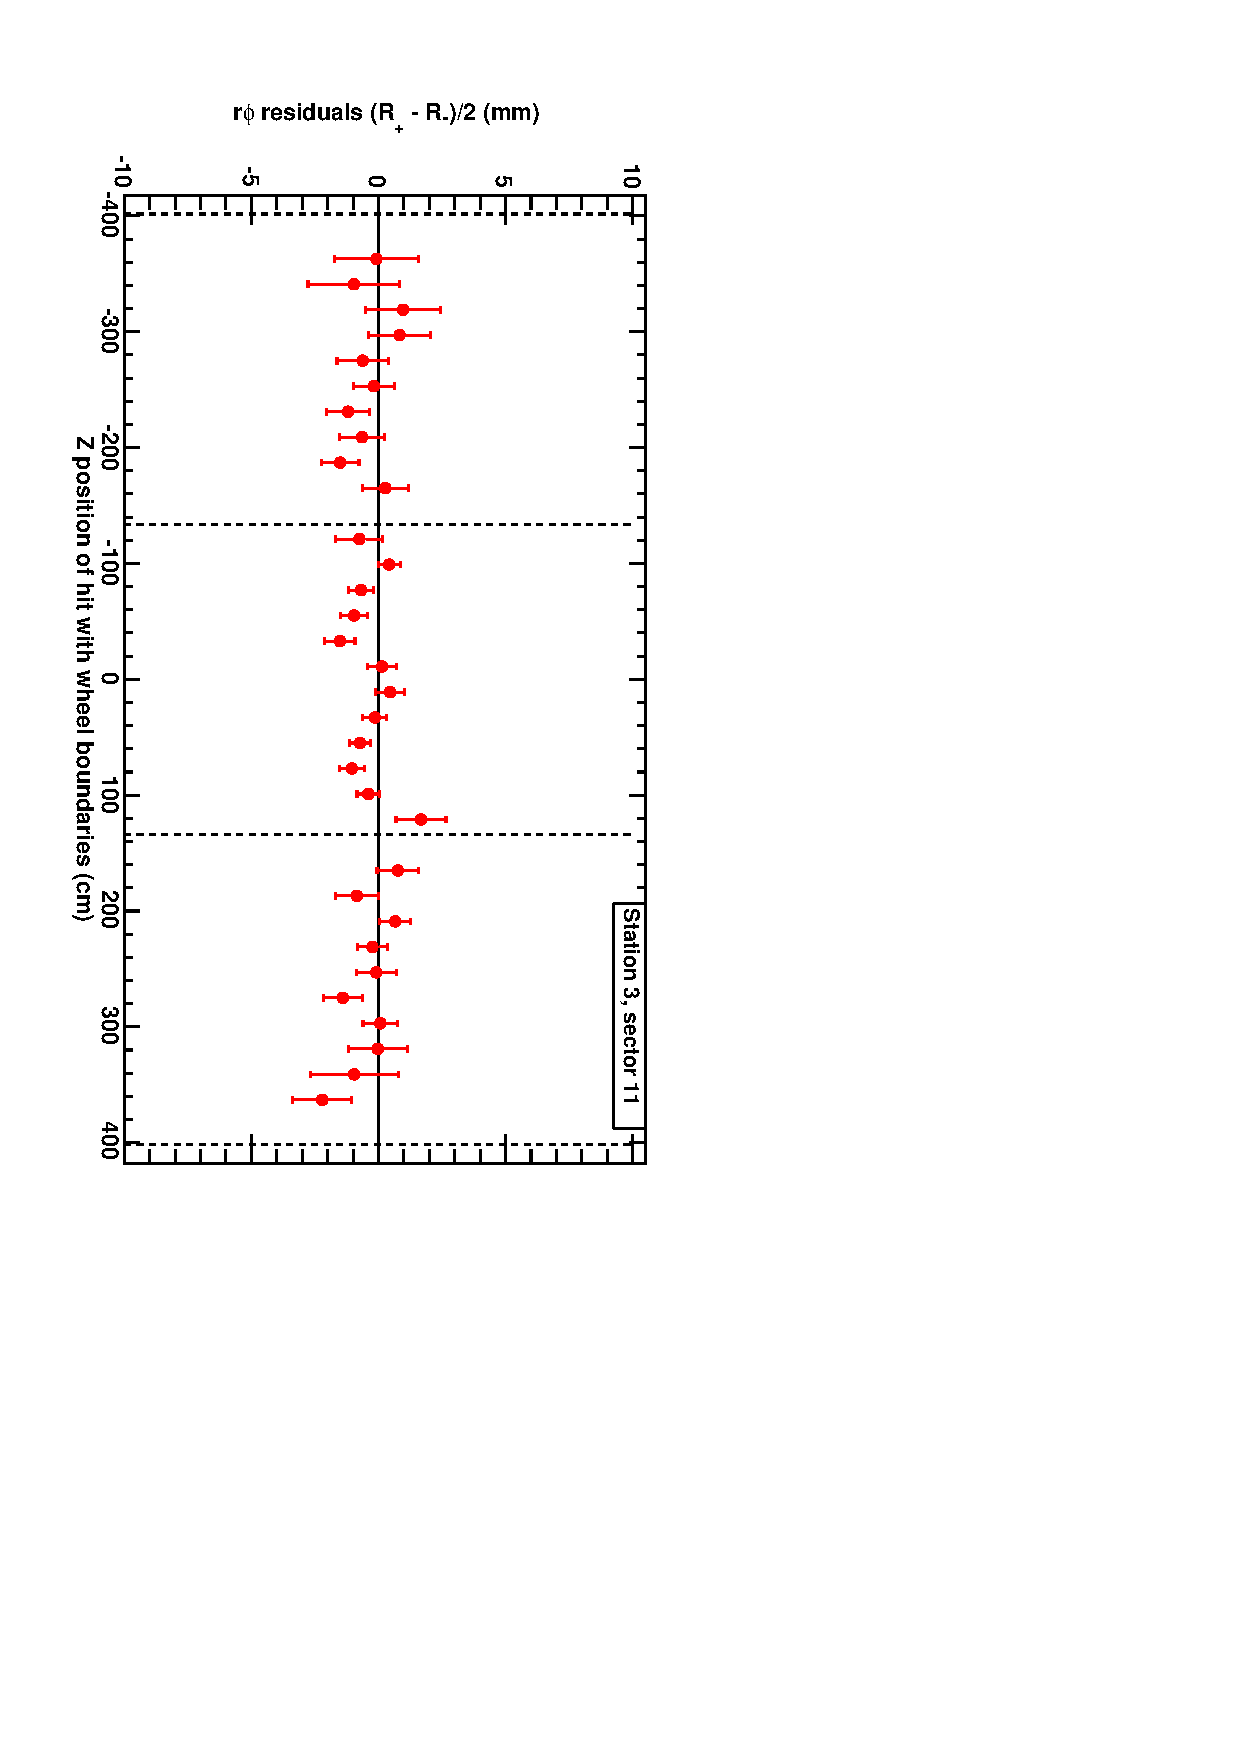
\includegraphics[height=0.28\linewidth, angle=90]{map40GeV_3_11.pdf}

\vspace{0.3 cm}
12.~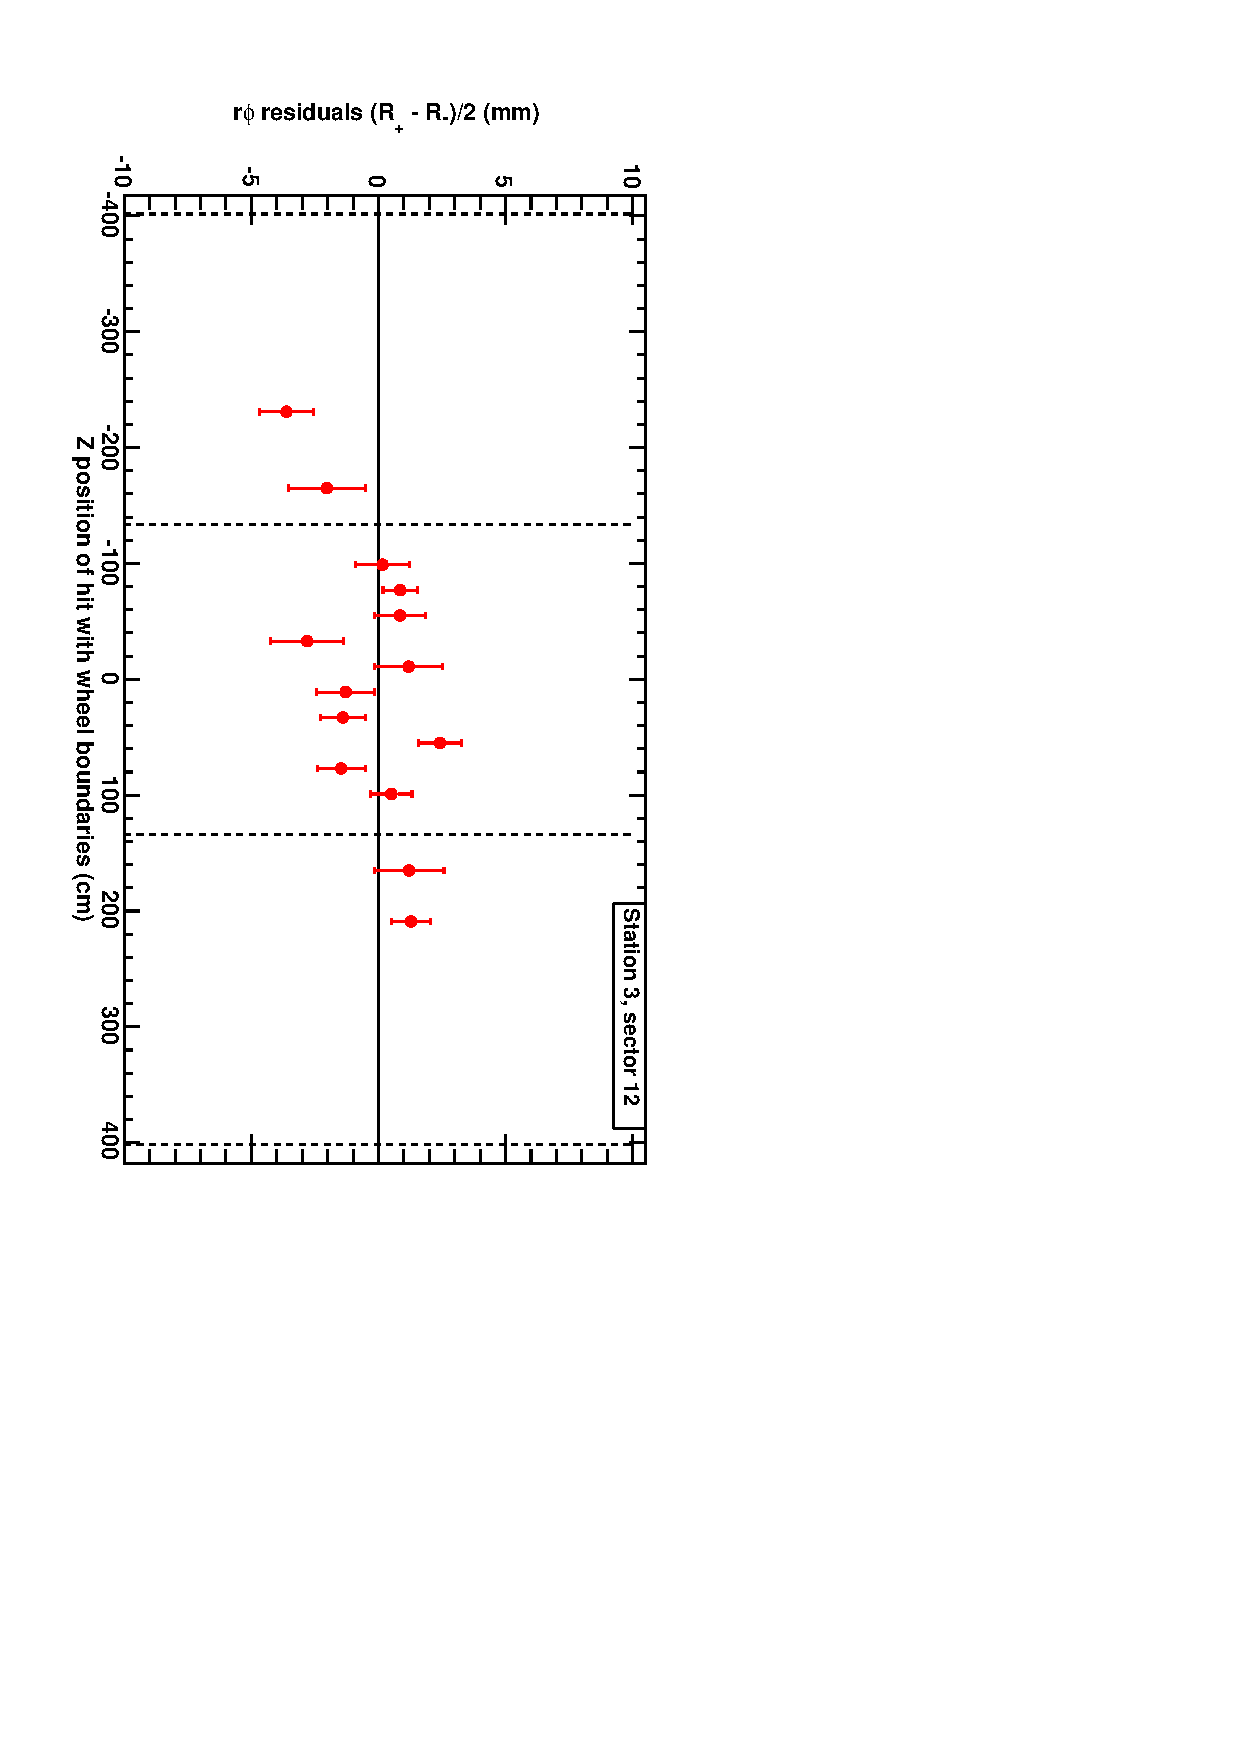
\includegraphics[height=0.28\linewidth, angle=90]{map40GeV_3_12.pdf}
\end{frame}

\begin{frame}
\frametitle{Individual bins vs.~$z$}
\framesubtitle{Station 4 (positive $-$ negative)/2 versus $z$}

2.~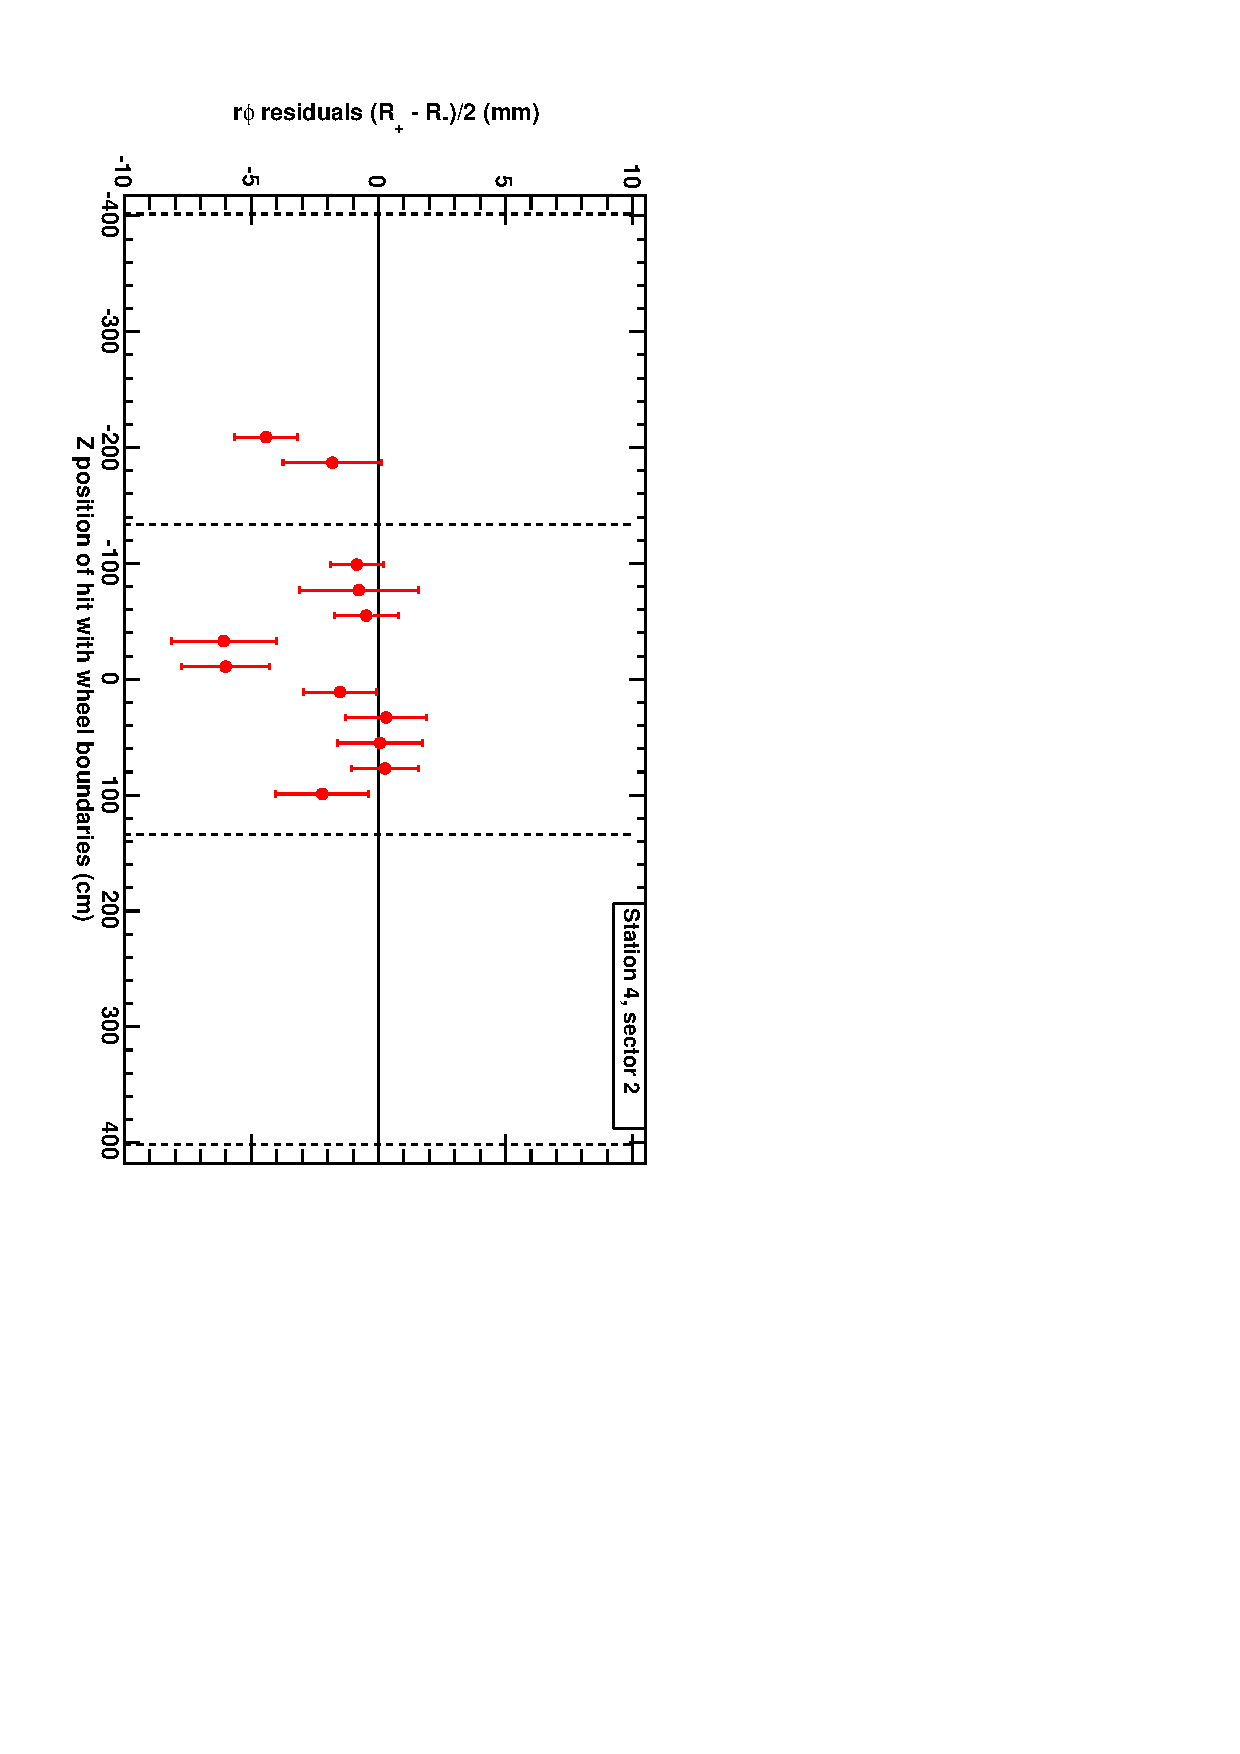
\includegraphics[height=0.28\linewidth, angle=90]{map40GeV_4_2.pdf} \hfill
3.~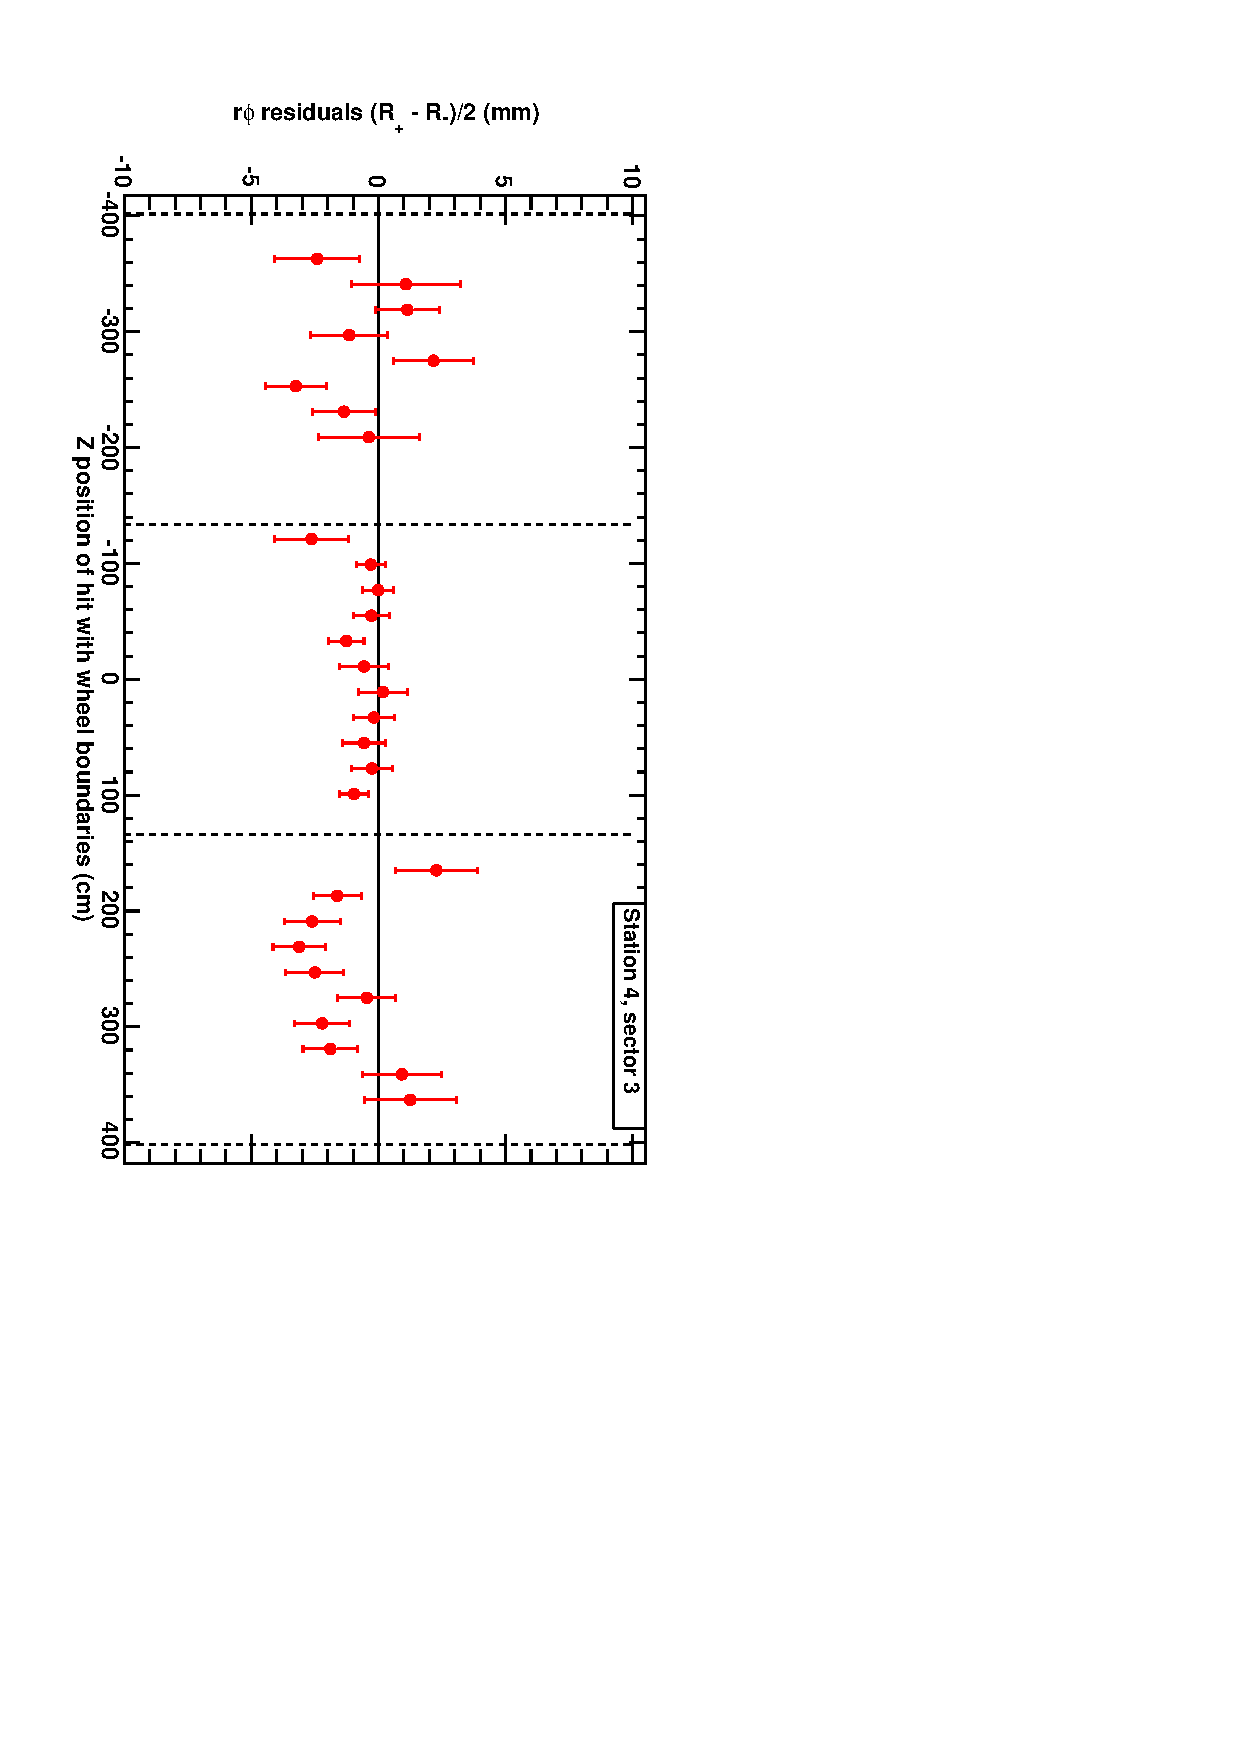
\includegraphics[height=0.28\linewidth, angle=90]{map40GeV_4_3.pdf} \hfill
4.~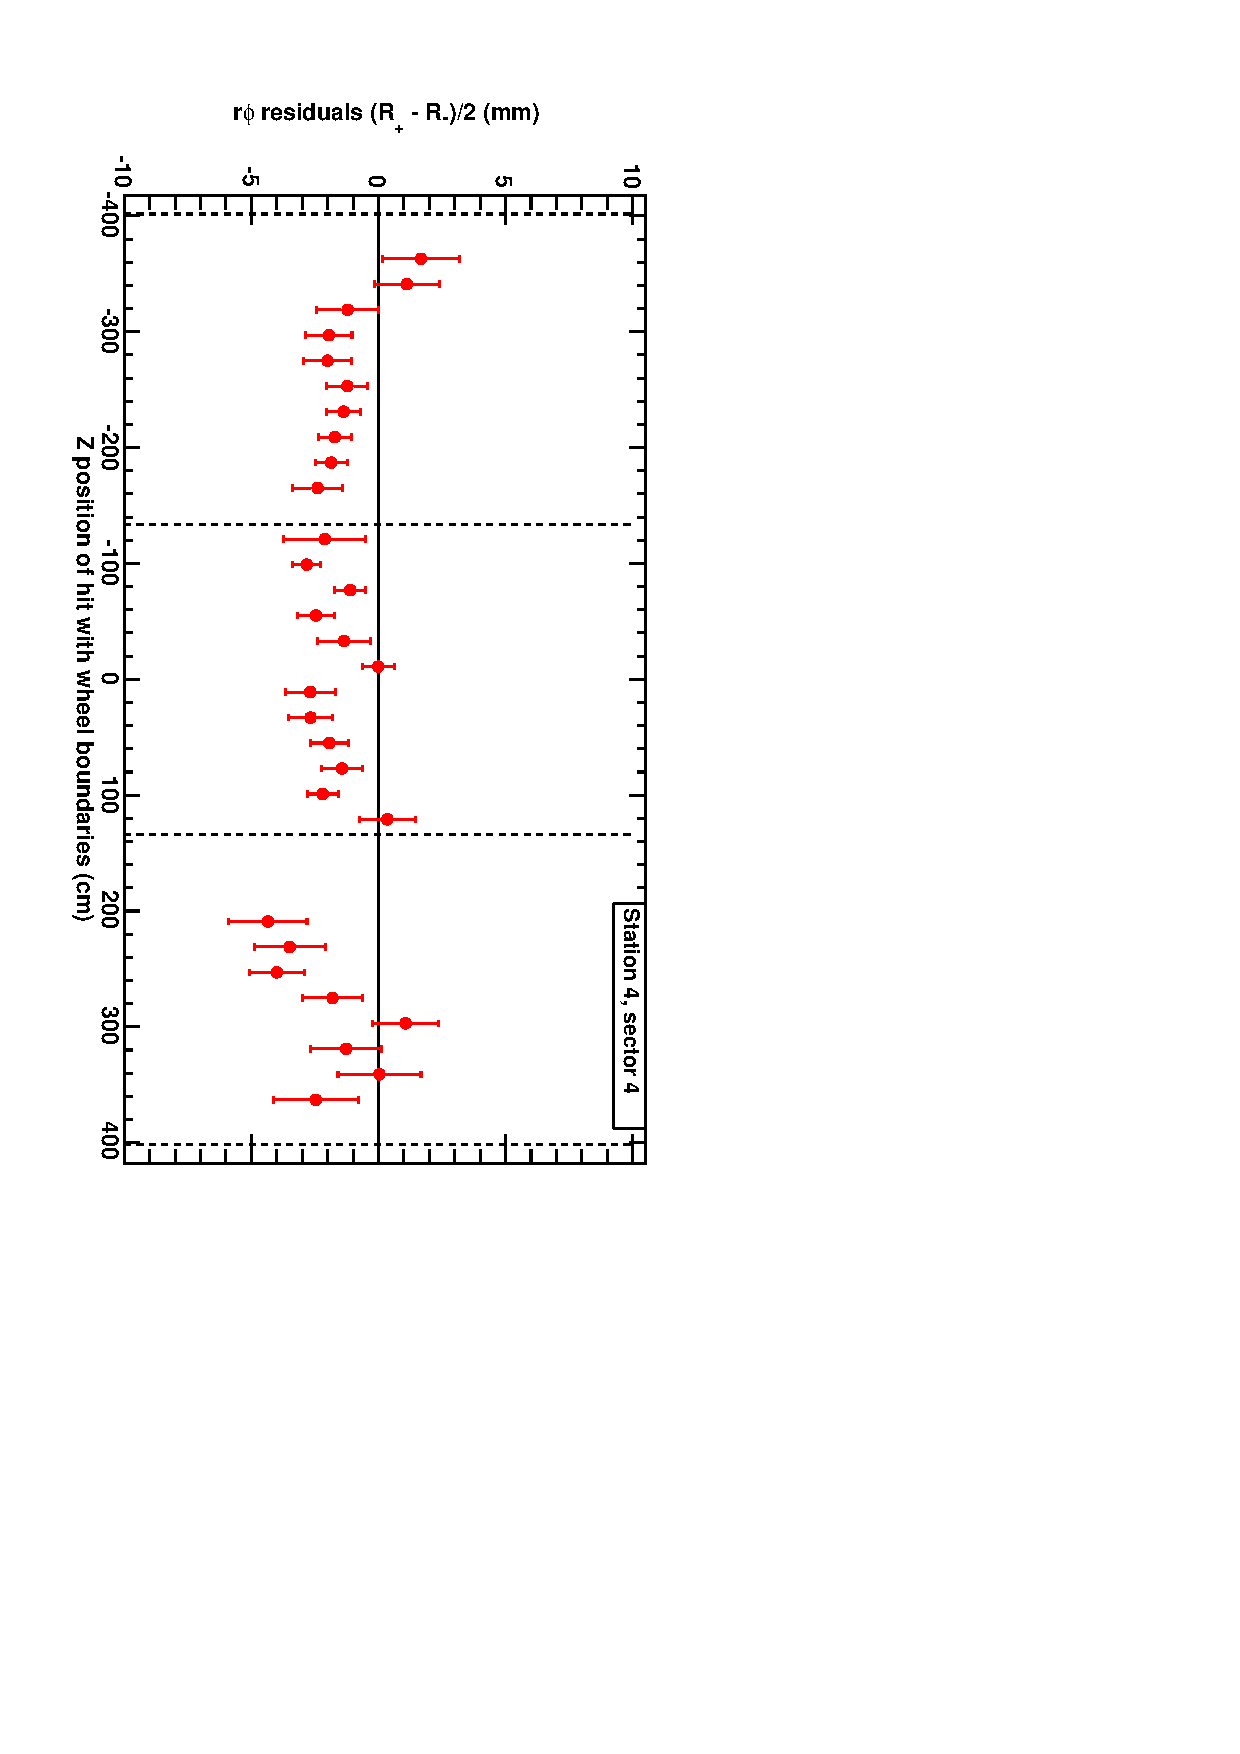
\includegraphics[height=0.28\linewidth, angle=90]{map40GeV_4_4.pdf}

\vspace{0.3 cm}
13.~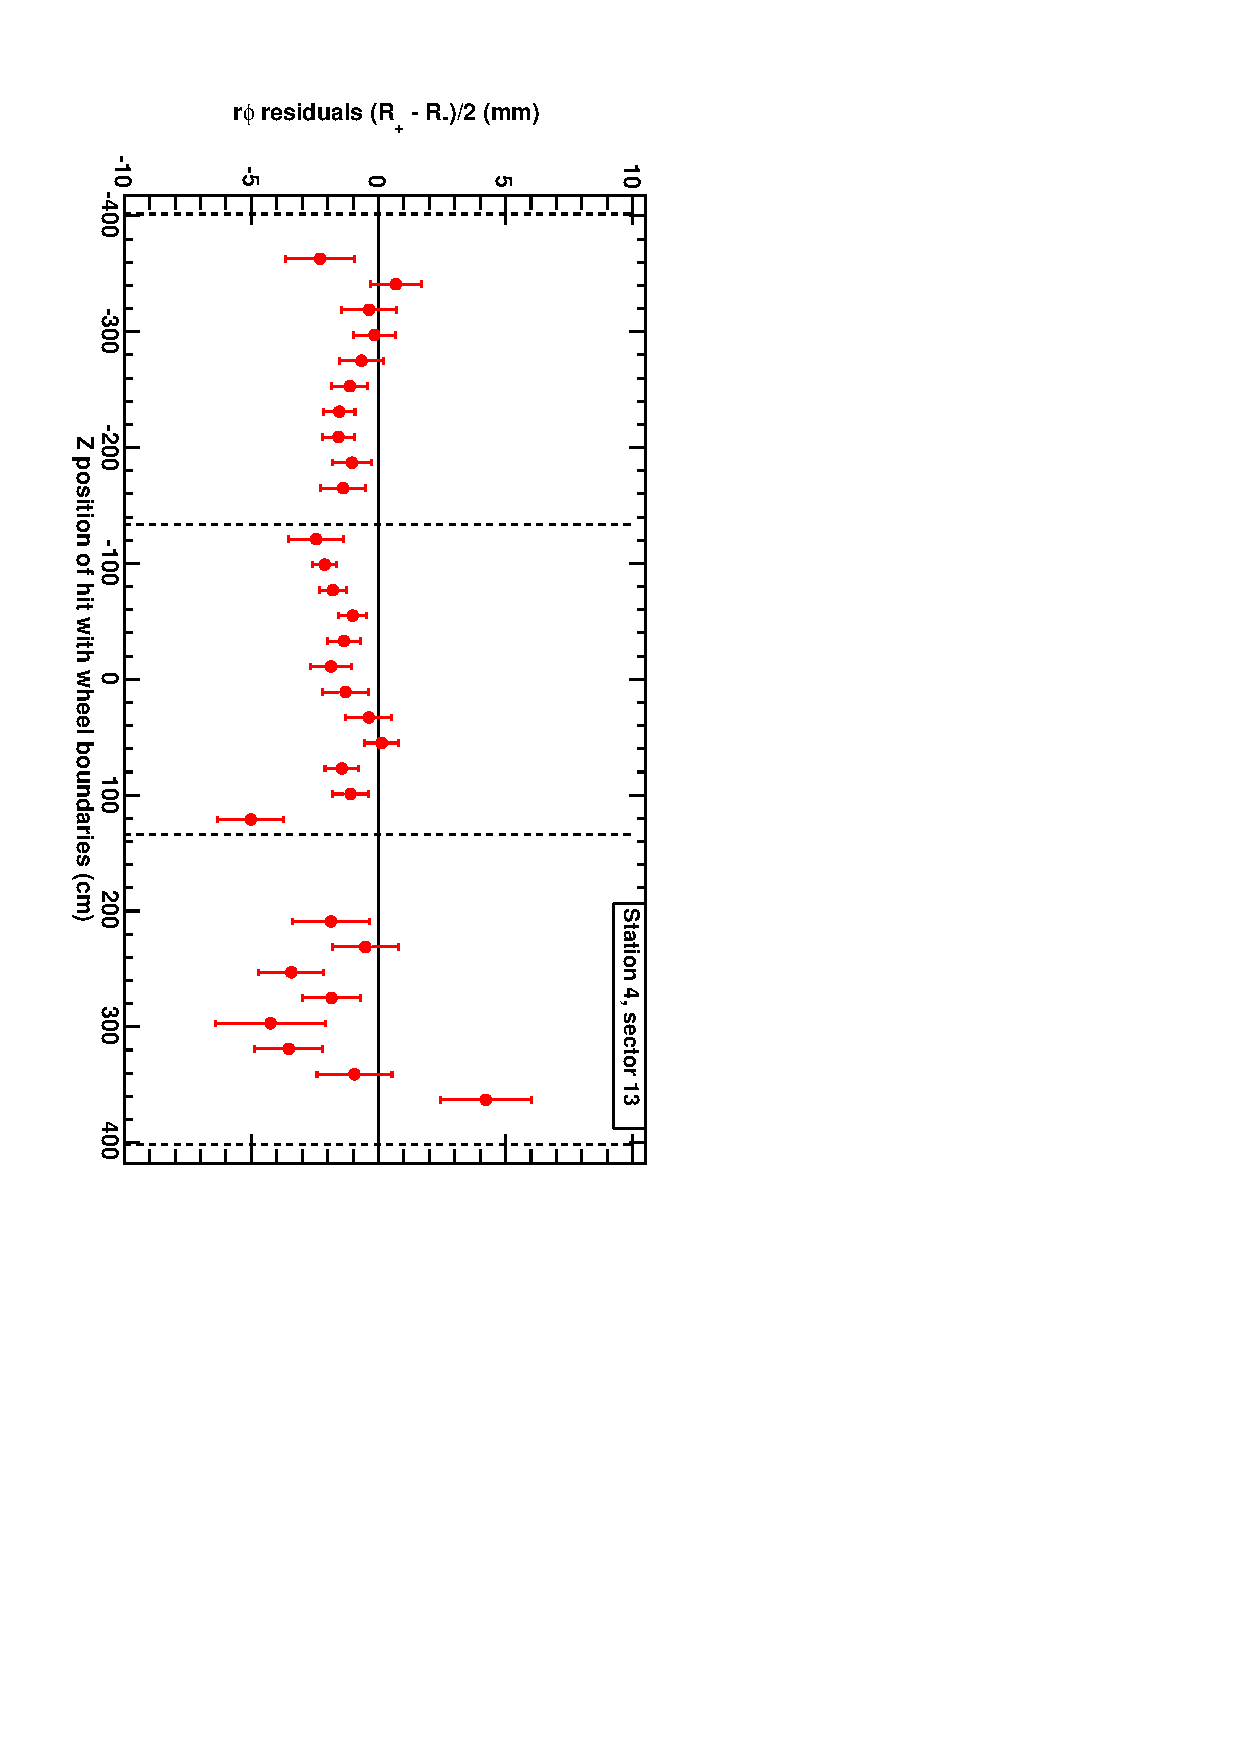
\includegraphics[height=0.28\linewidth, angle=90]{map40GeV_4_13.pdf} \hfill
5.~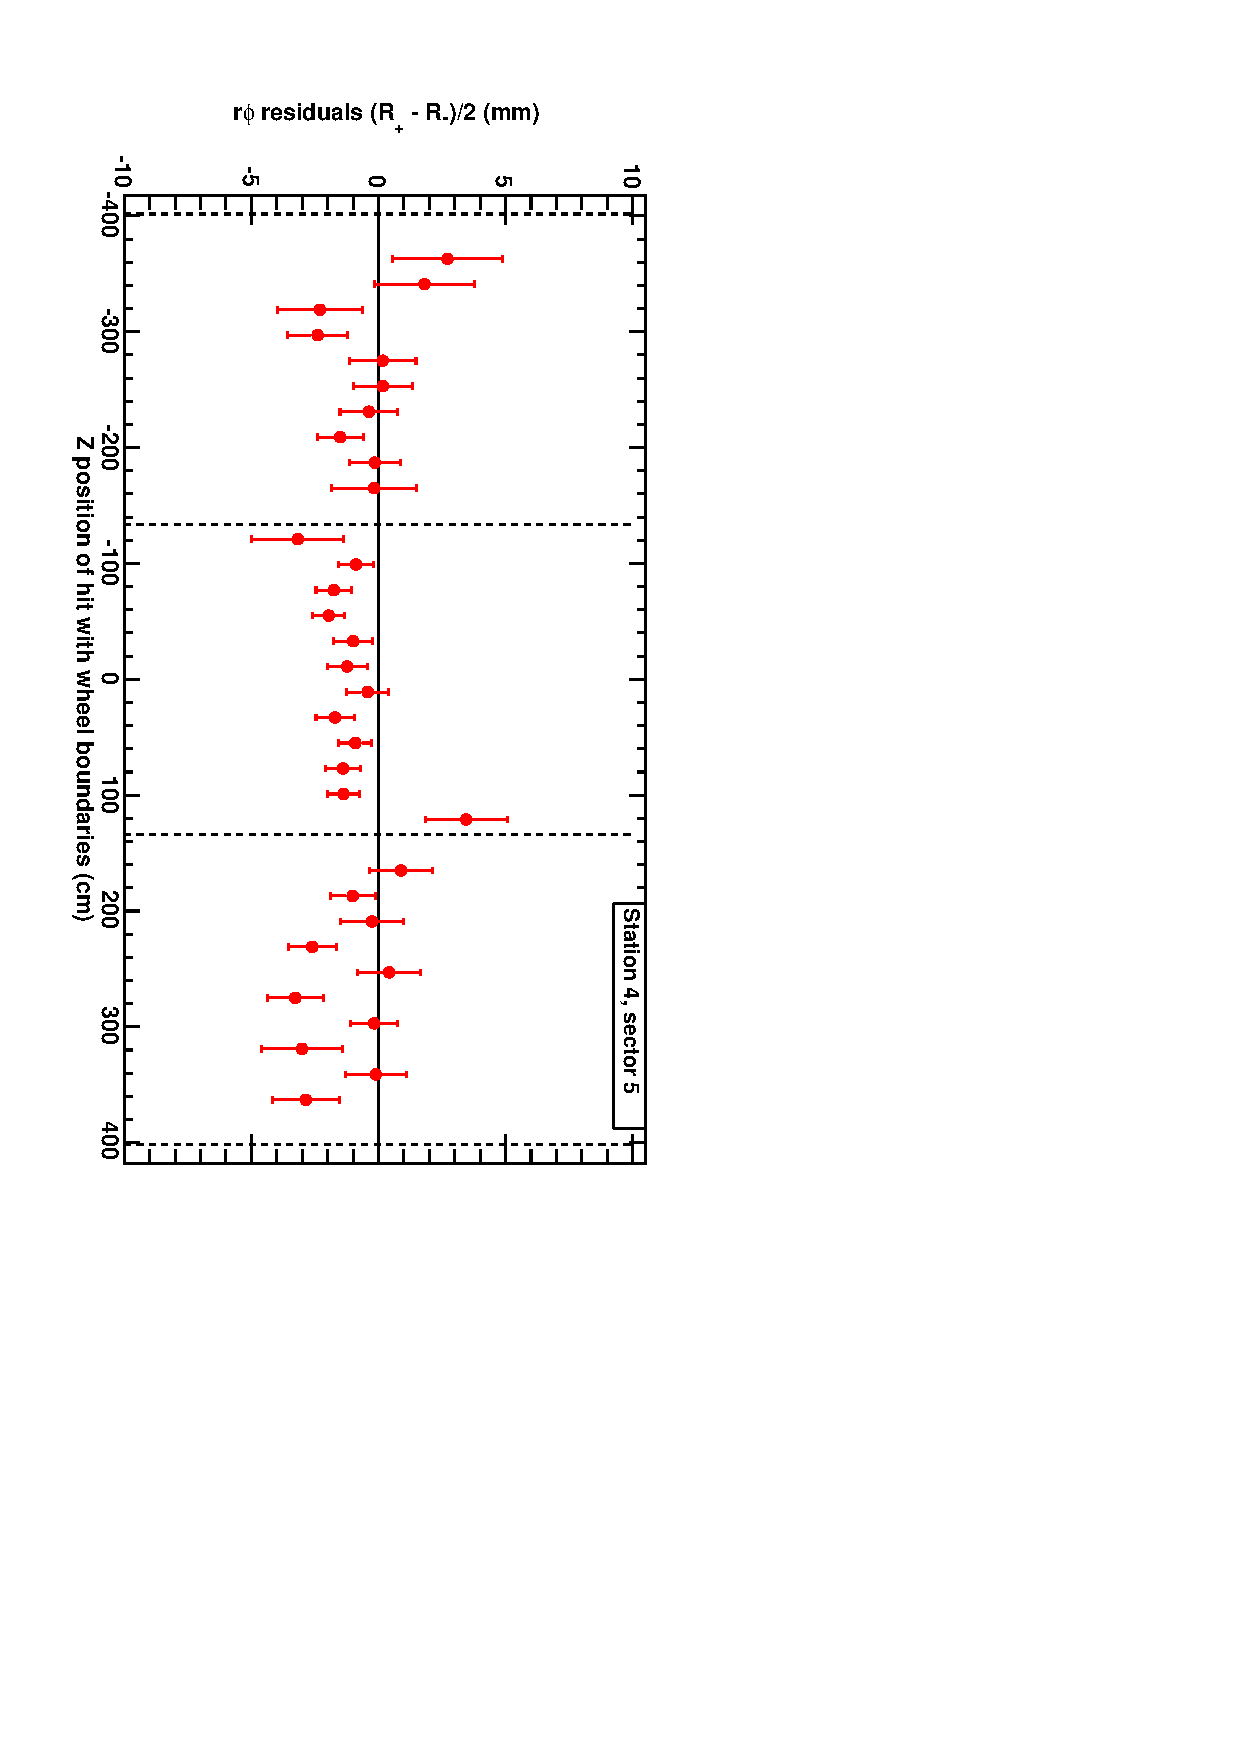
\includegraphics[height=0.28\linewidth, angle=90]{map40GeV_4_5.pdf} \hfill
6.~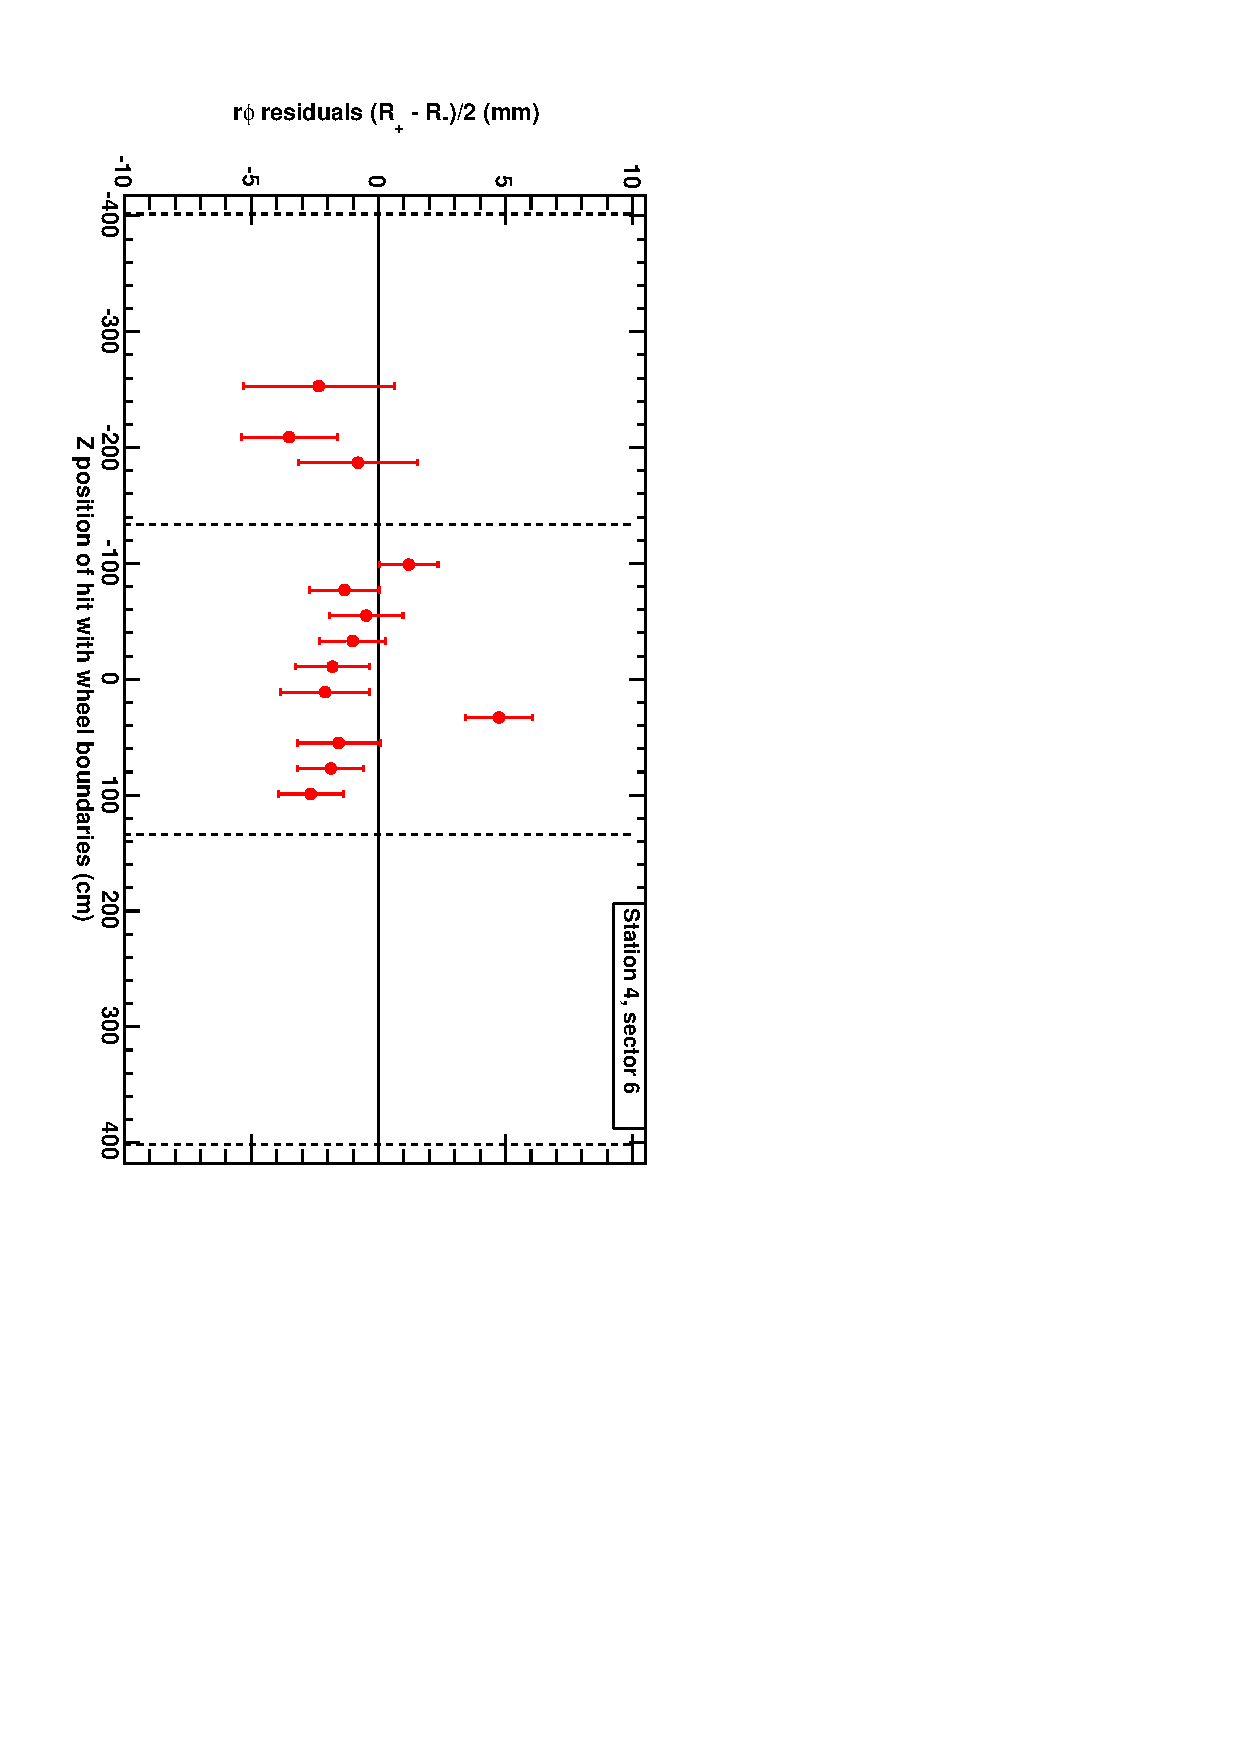
\includegraphics[height=0.28\linewidth, angle=90]{map40GeV_4_6.pdf} \hfill

\vspace{0.3 cm}
8.~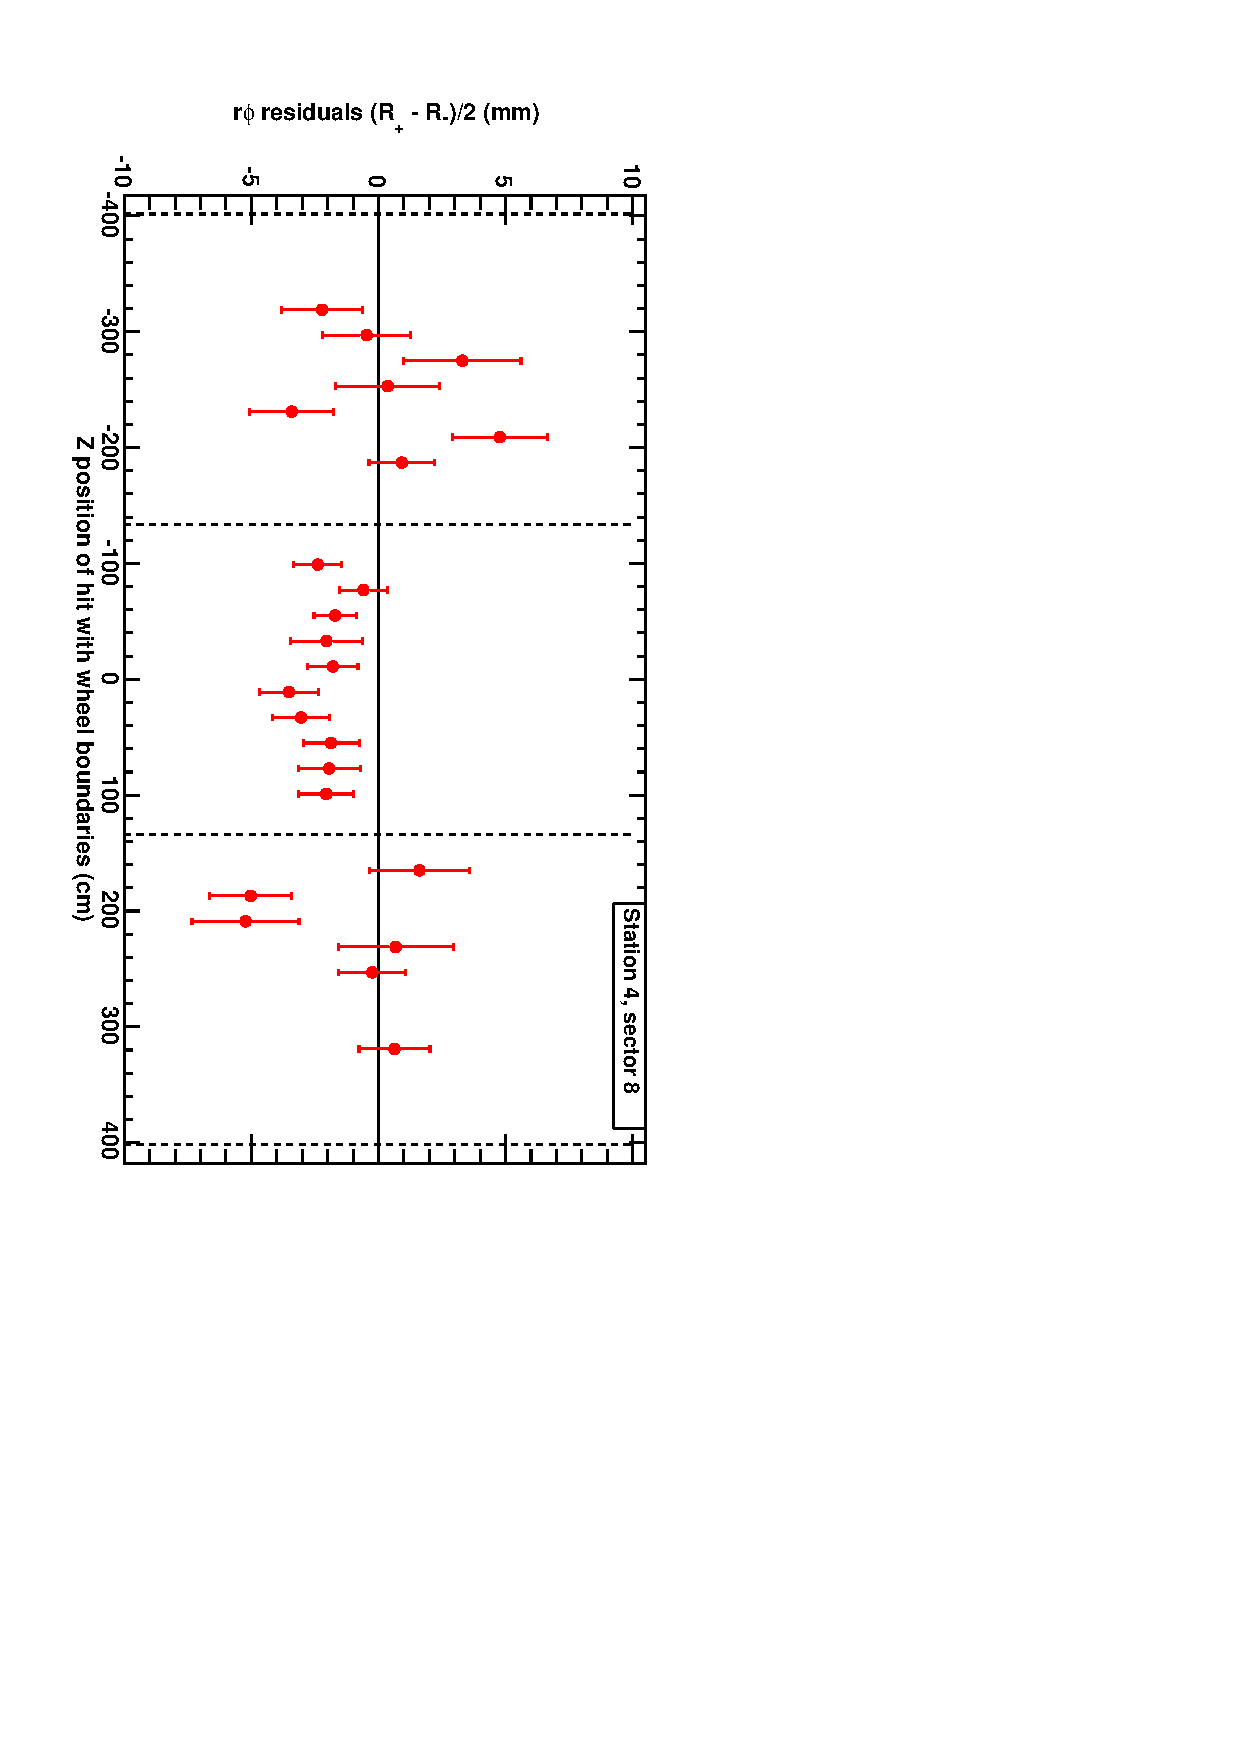
\includegraphics[height=0.28\linewidth, angle=90]{map40GeV_4_8.pdf}
9.~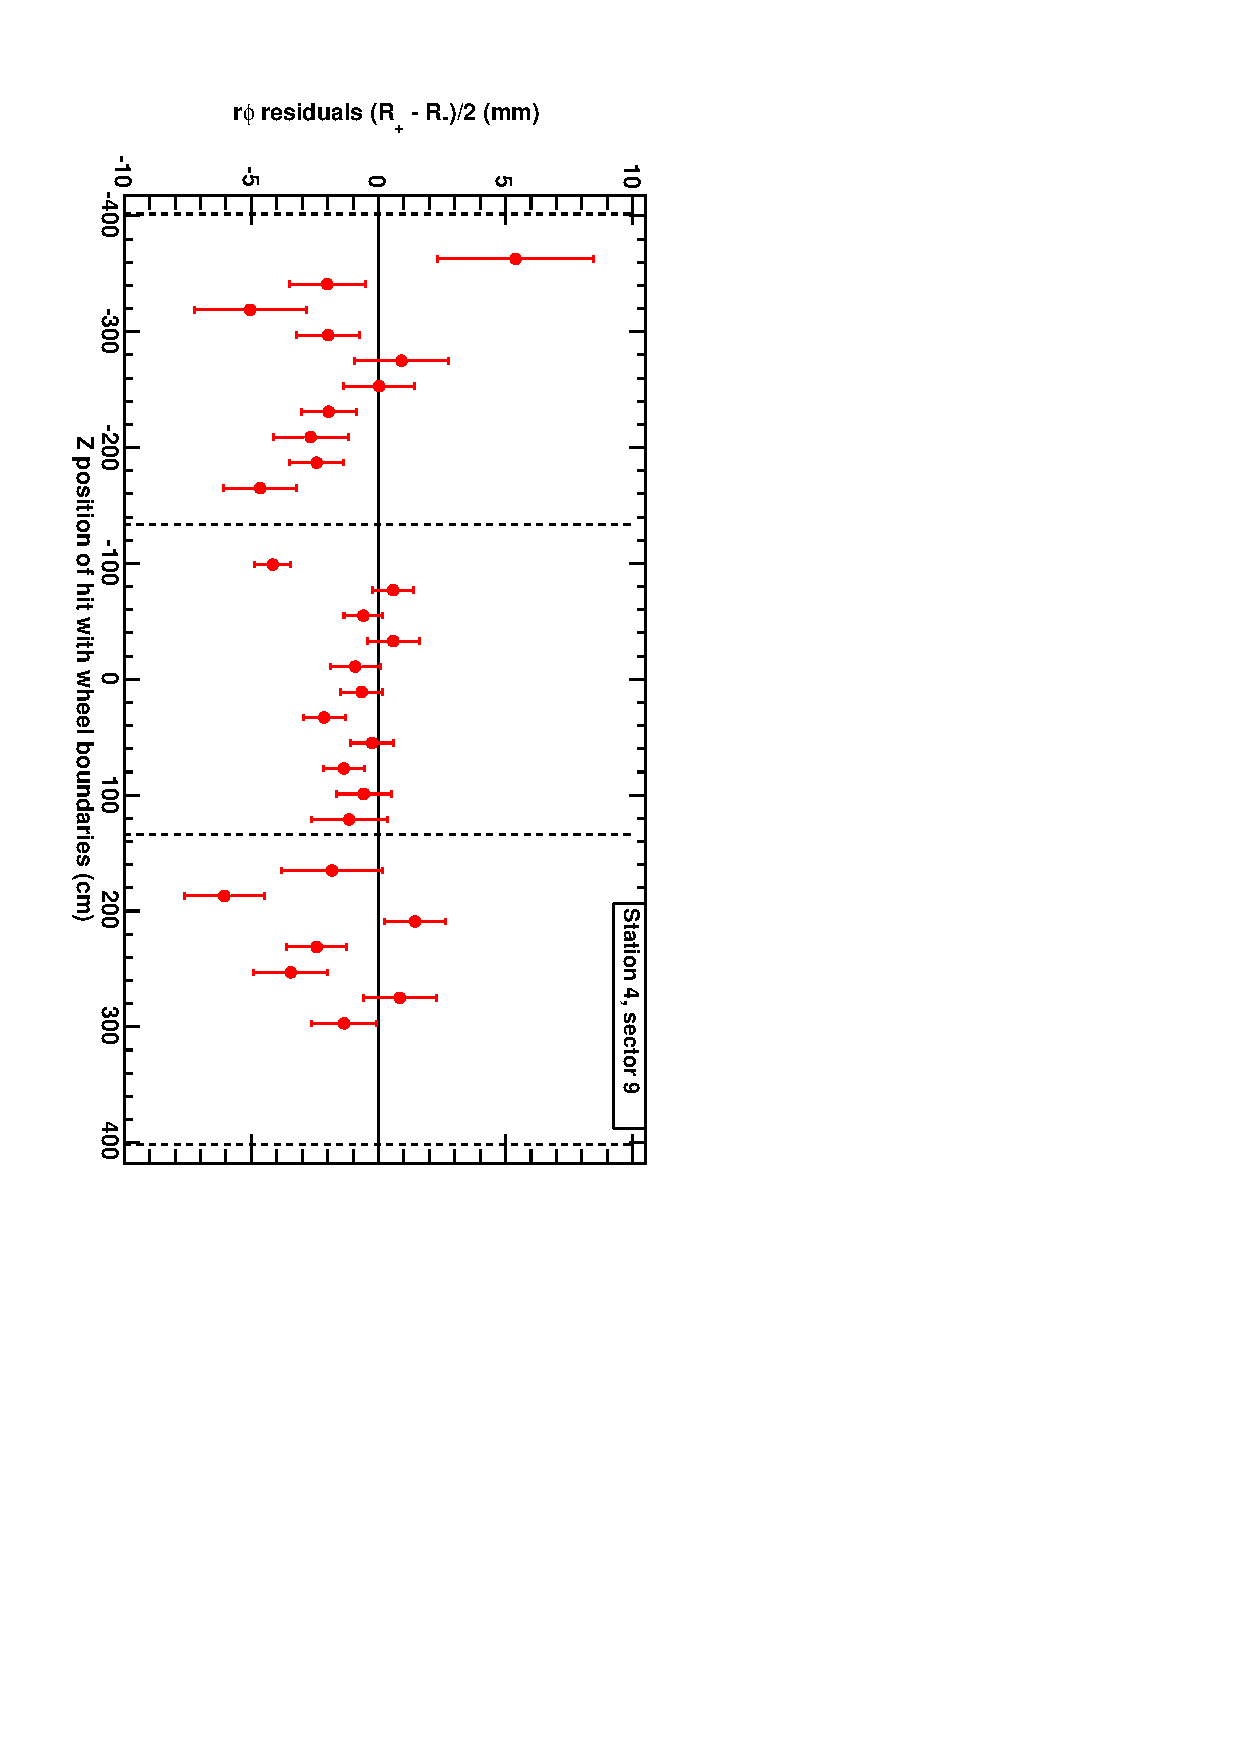
\includegraphics[height=0.28\linewidth, angle=90]{map40GeV_4_9.pdf} \hfill
10.~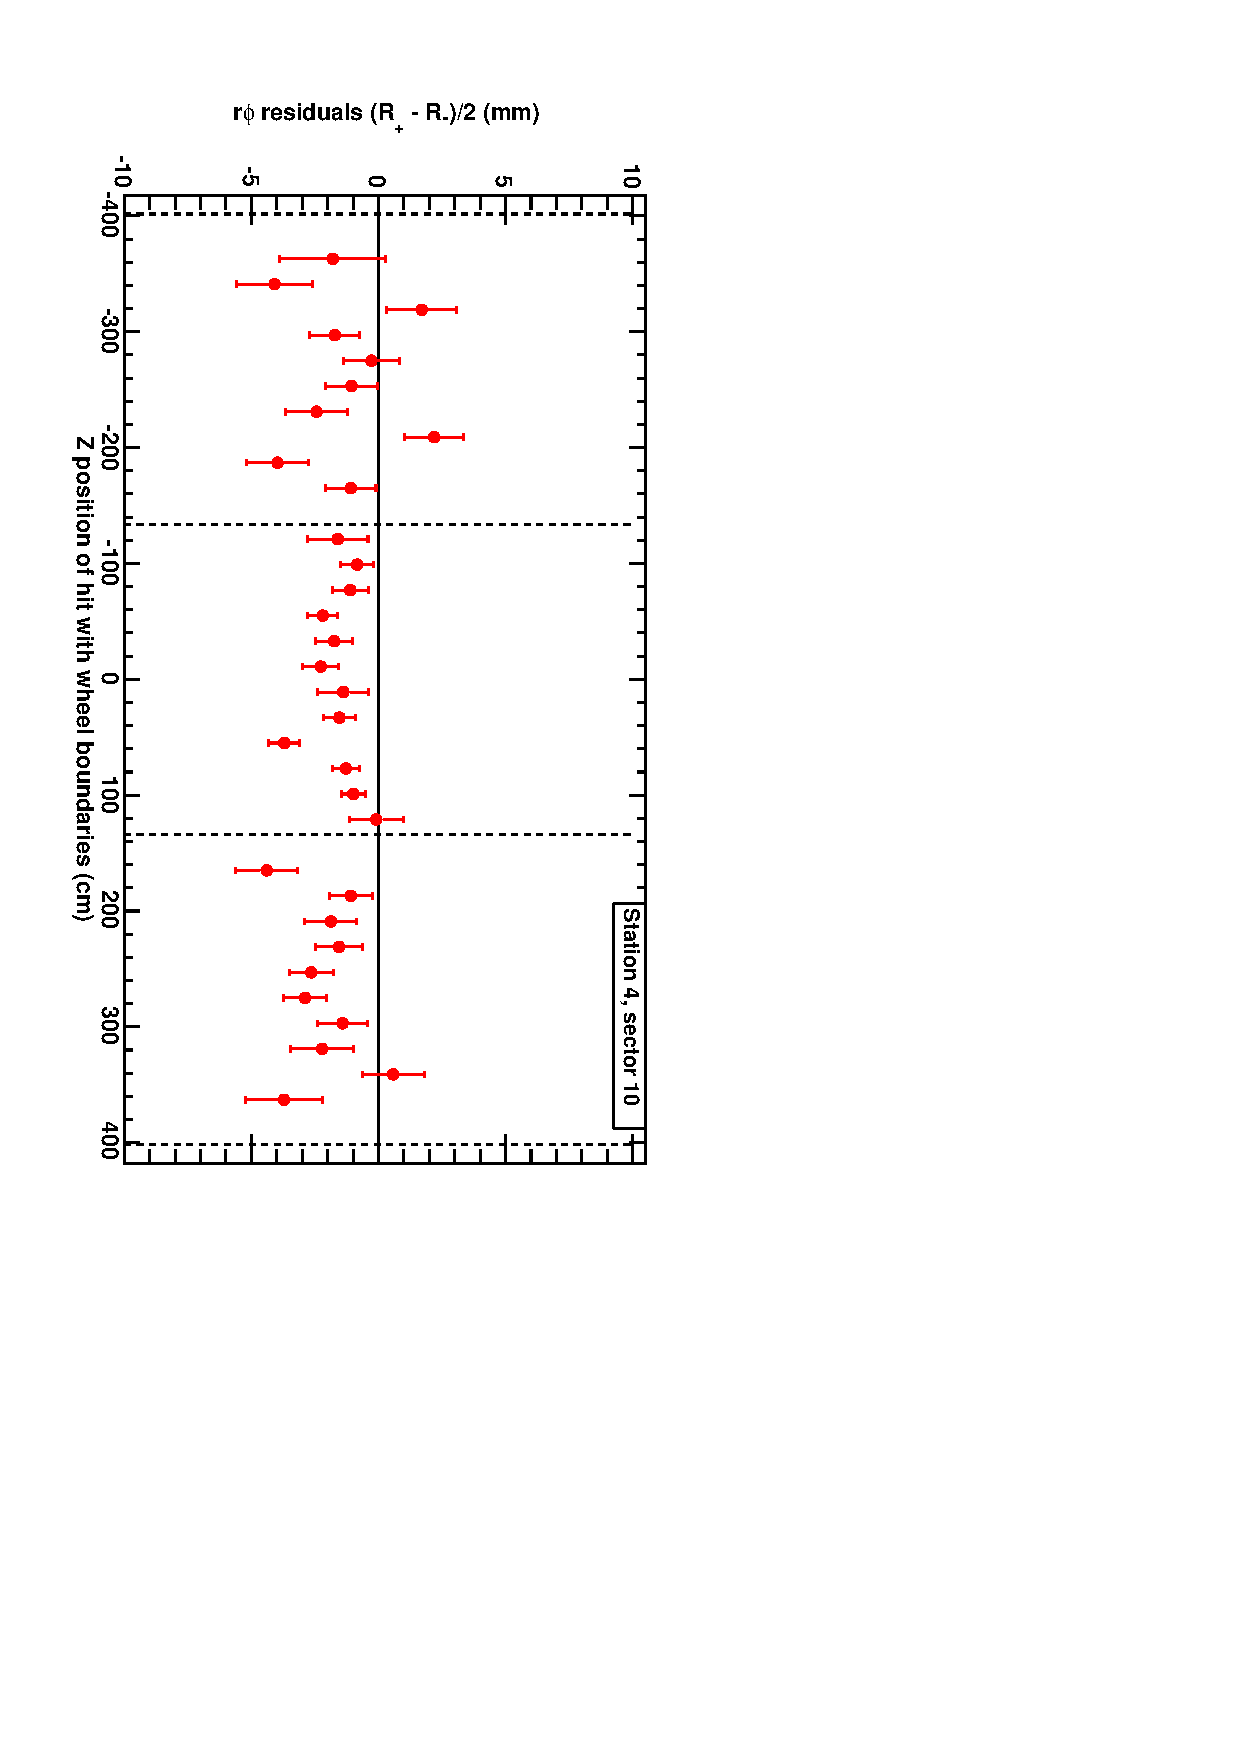
\includegraphics[height=0.28\linewidth, angle=90]{map40GeV_4_10.pdf} \hfill

\vspace{0.3 cm}
14.~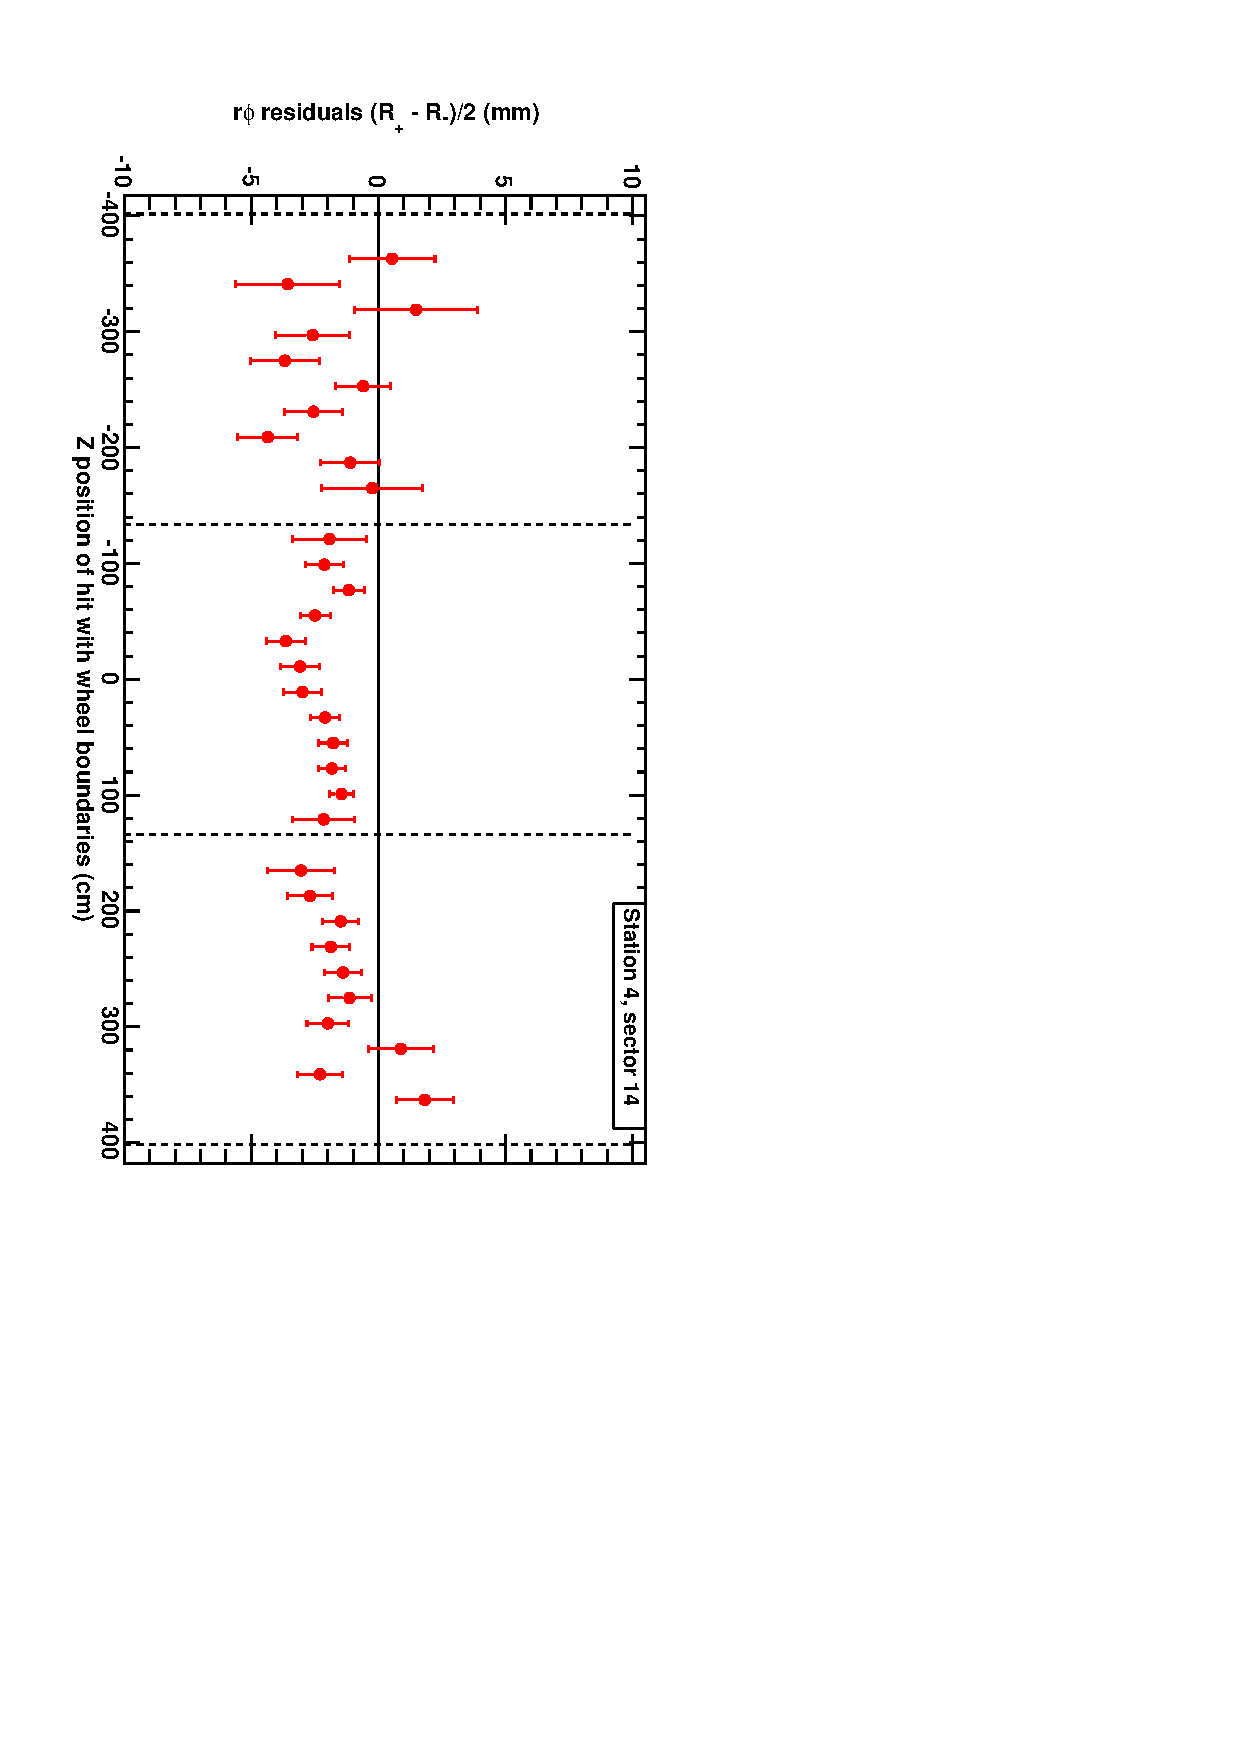
\includegraphics[height=0.28\linewidth, angle=90]{map40GeV_4_14.pdf} \hfill
11.~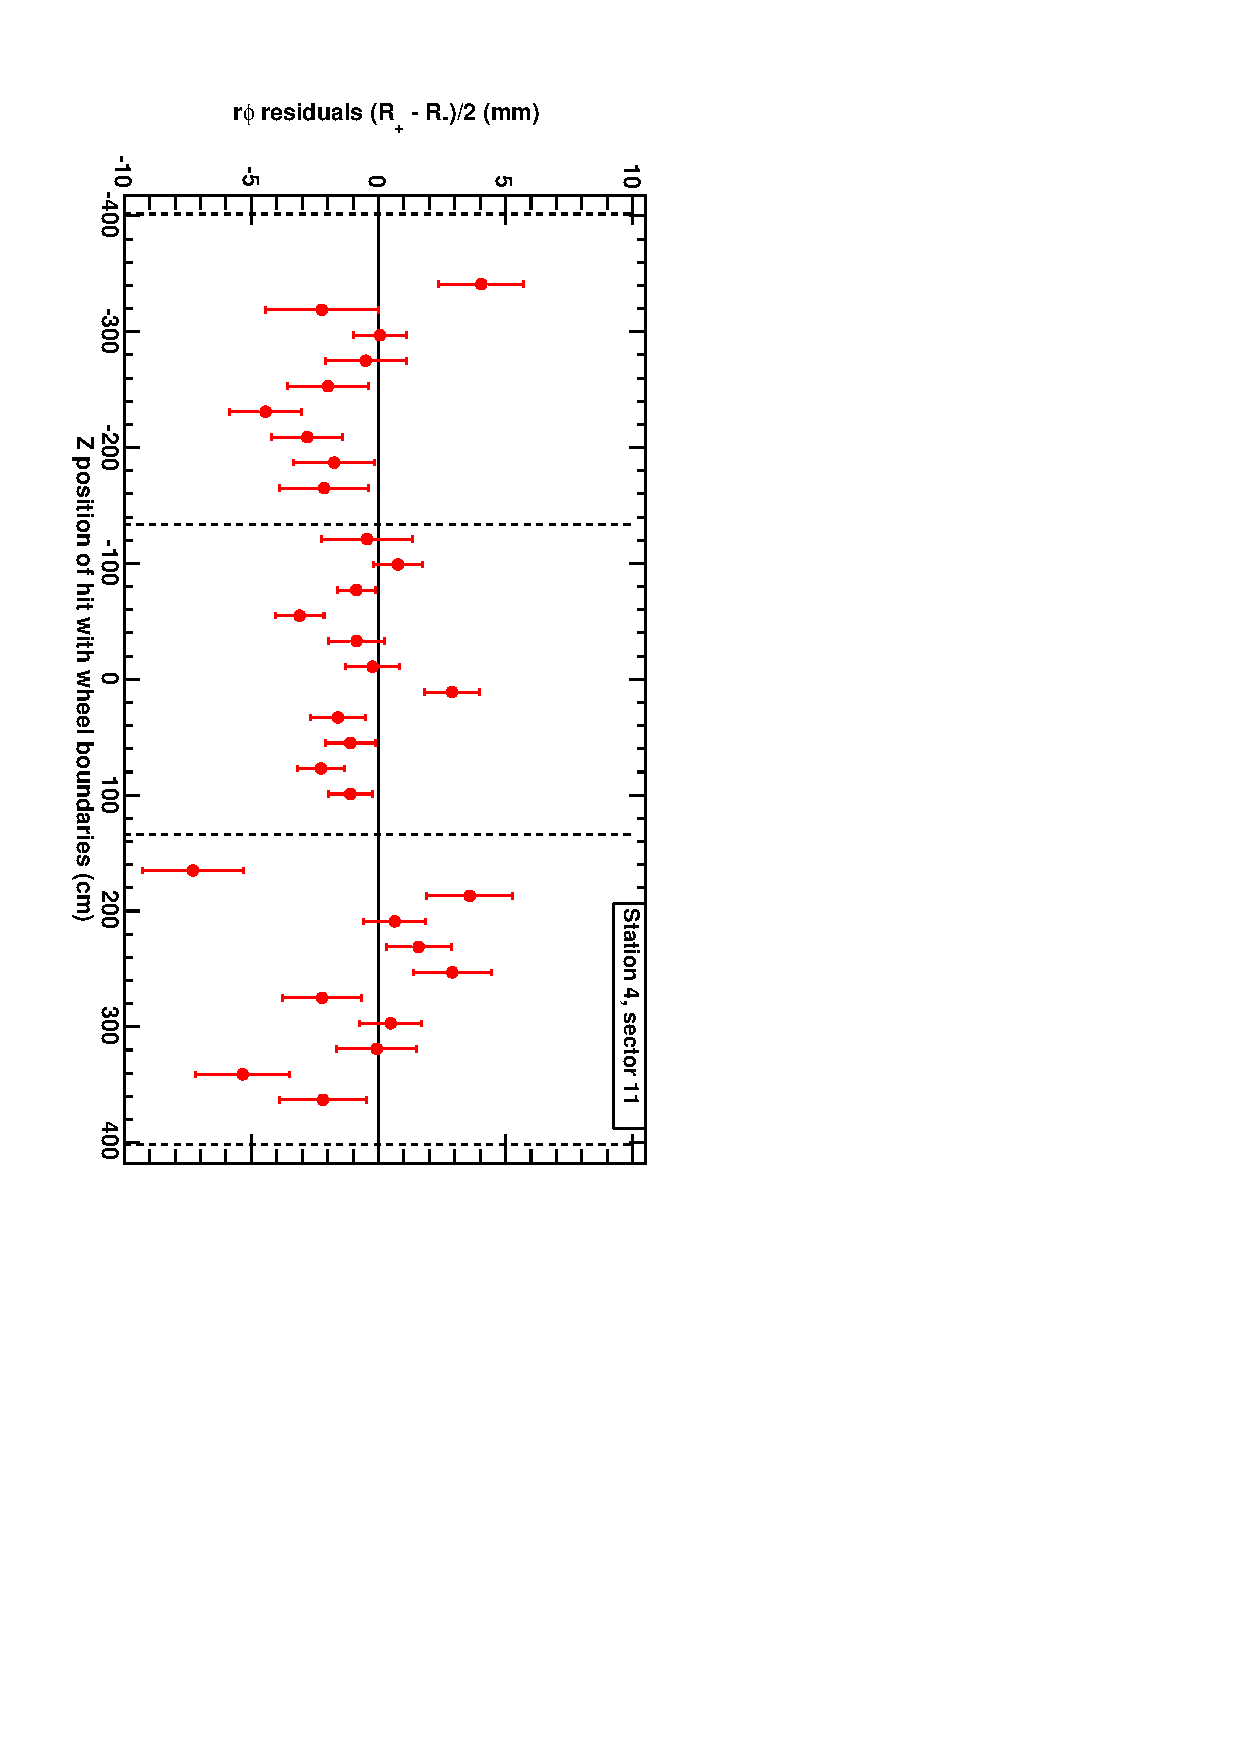
\includegraphics[height=0.28\linewidth, angle=90]{map40GeV_4_11.pdf}
12.~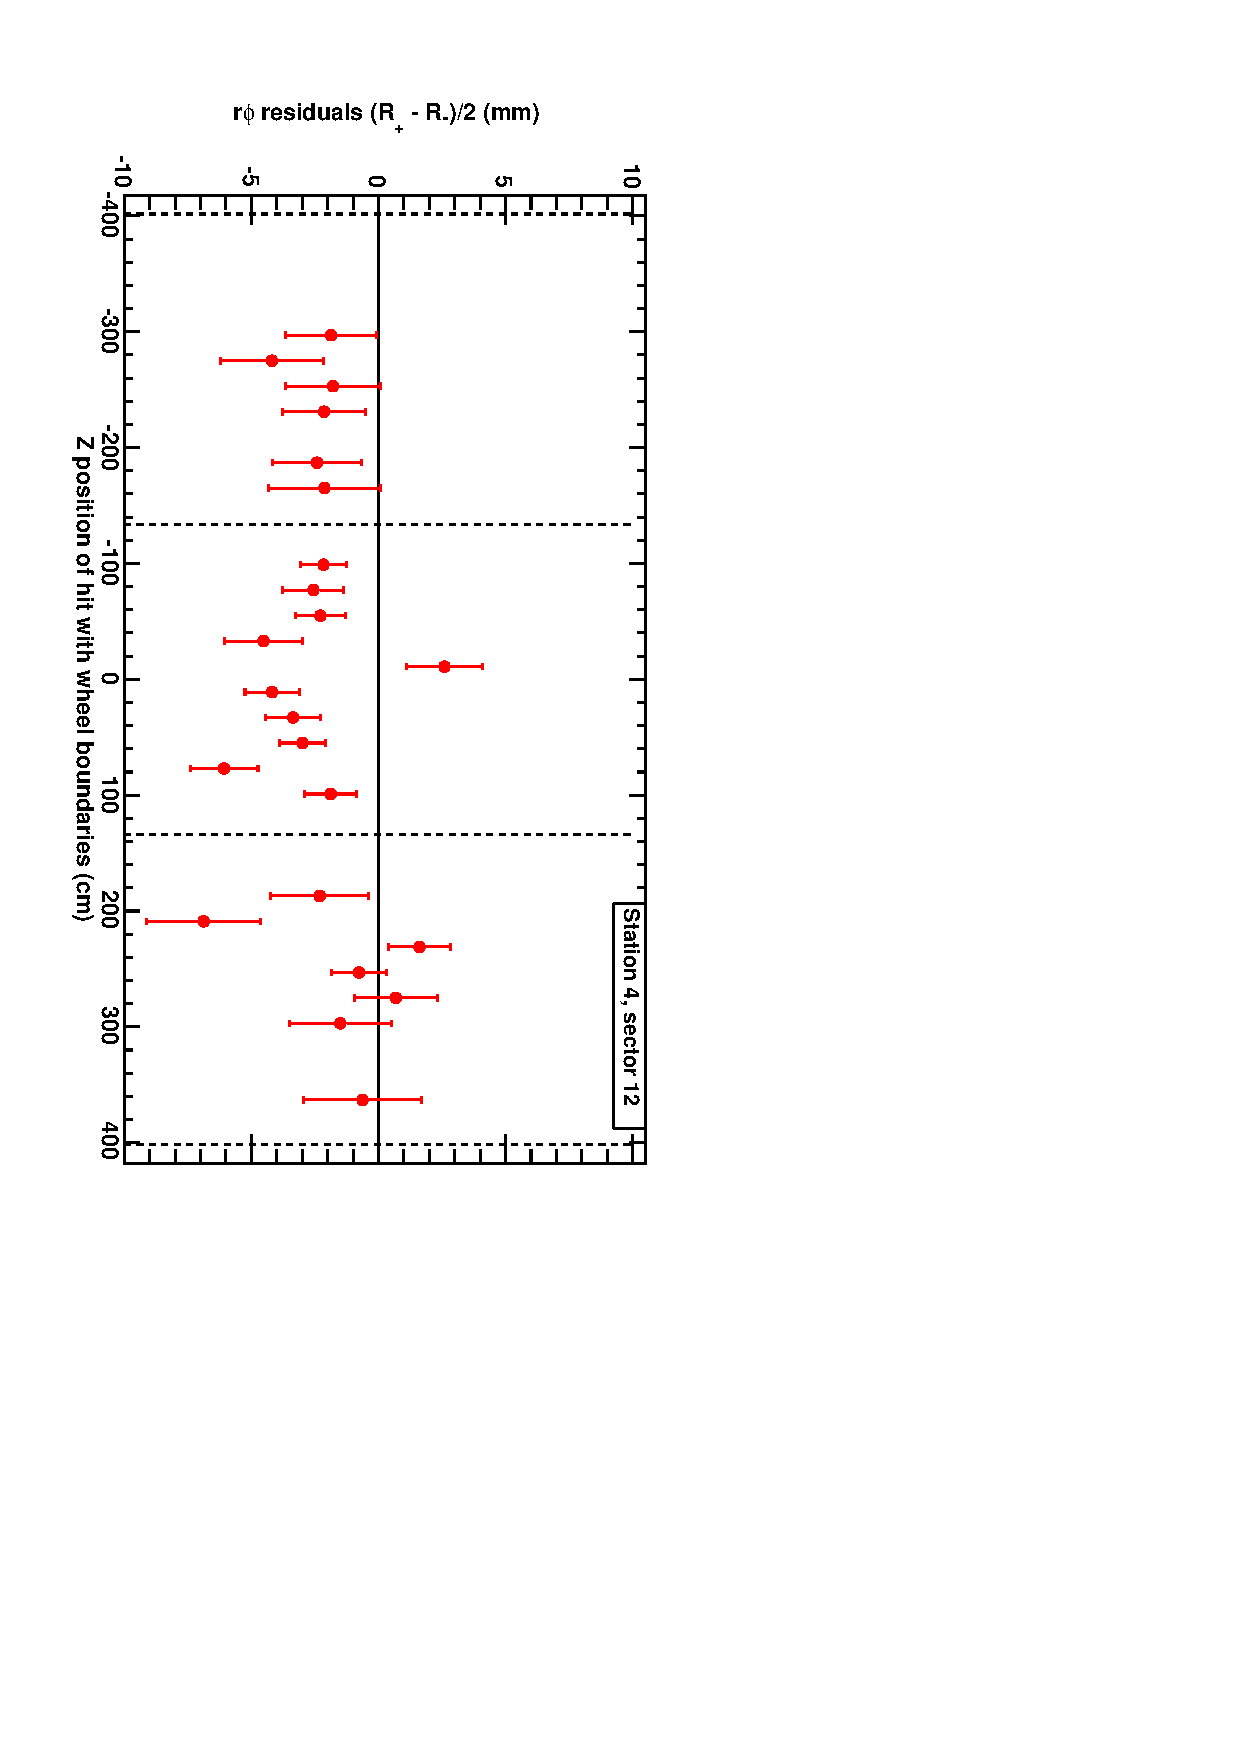
\includegraphics[height=0.28\linewidth, angle=90]{map40GeV_4_12.pdf}
\end{frame}

\begin{frame}
\frametitle{Results for $90 < p_T < 100$~GeV}

\begin{columns}
\column{0.7\linewidth}
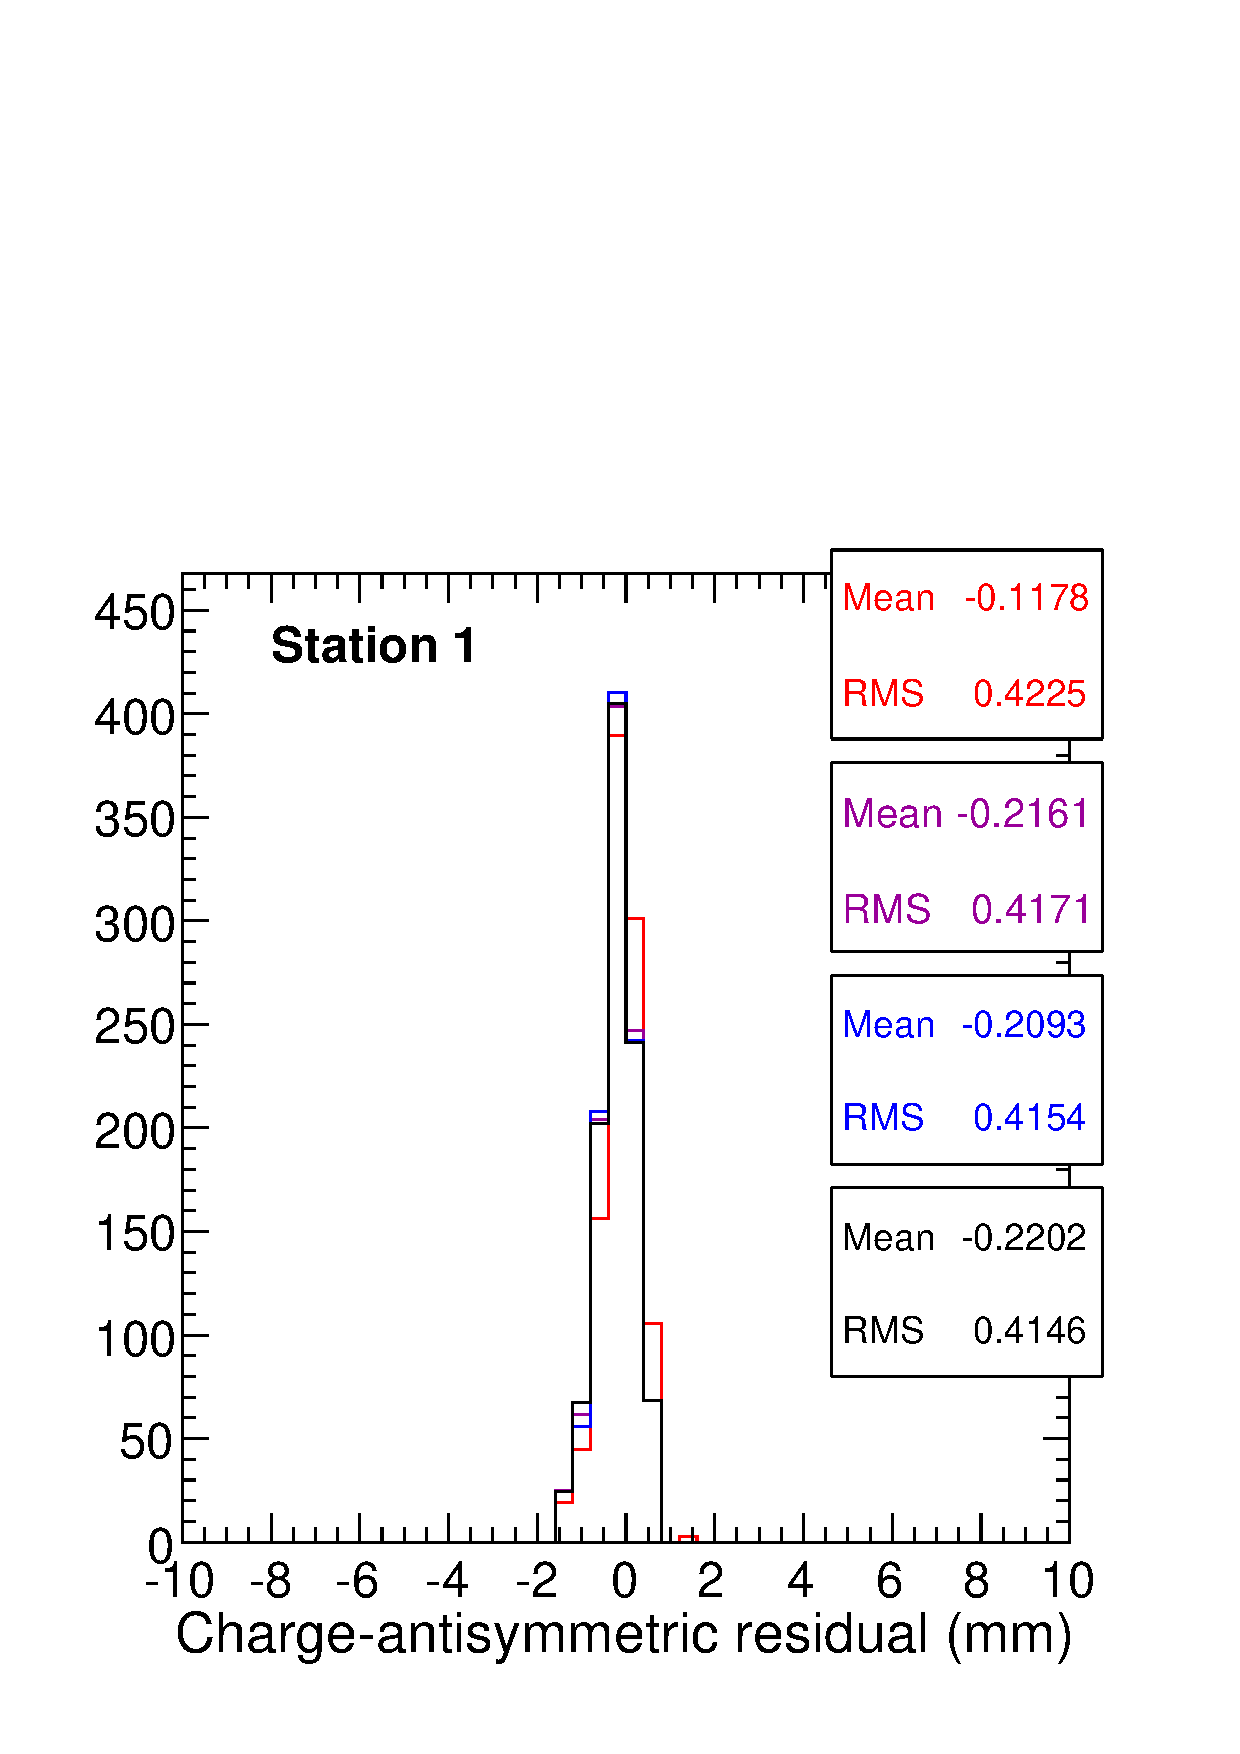
\includegraphics[width=0.5\linewidth]{station1_ptcut90.pdf}
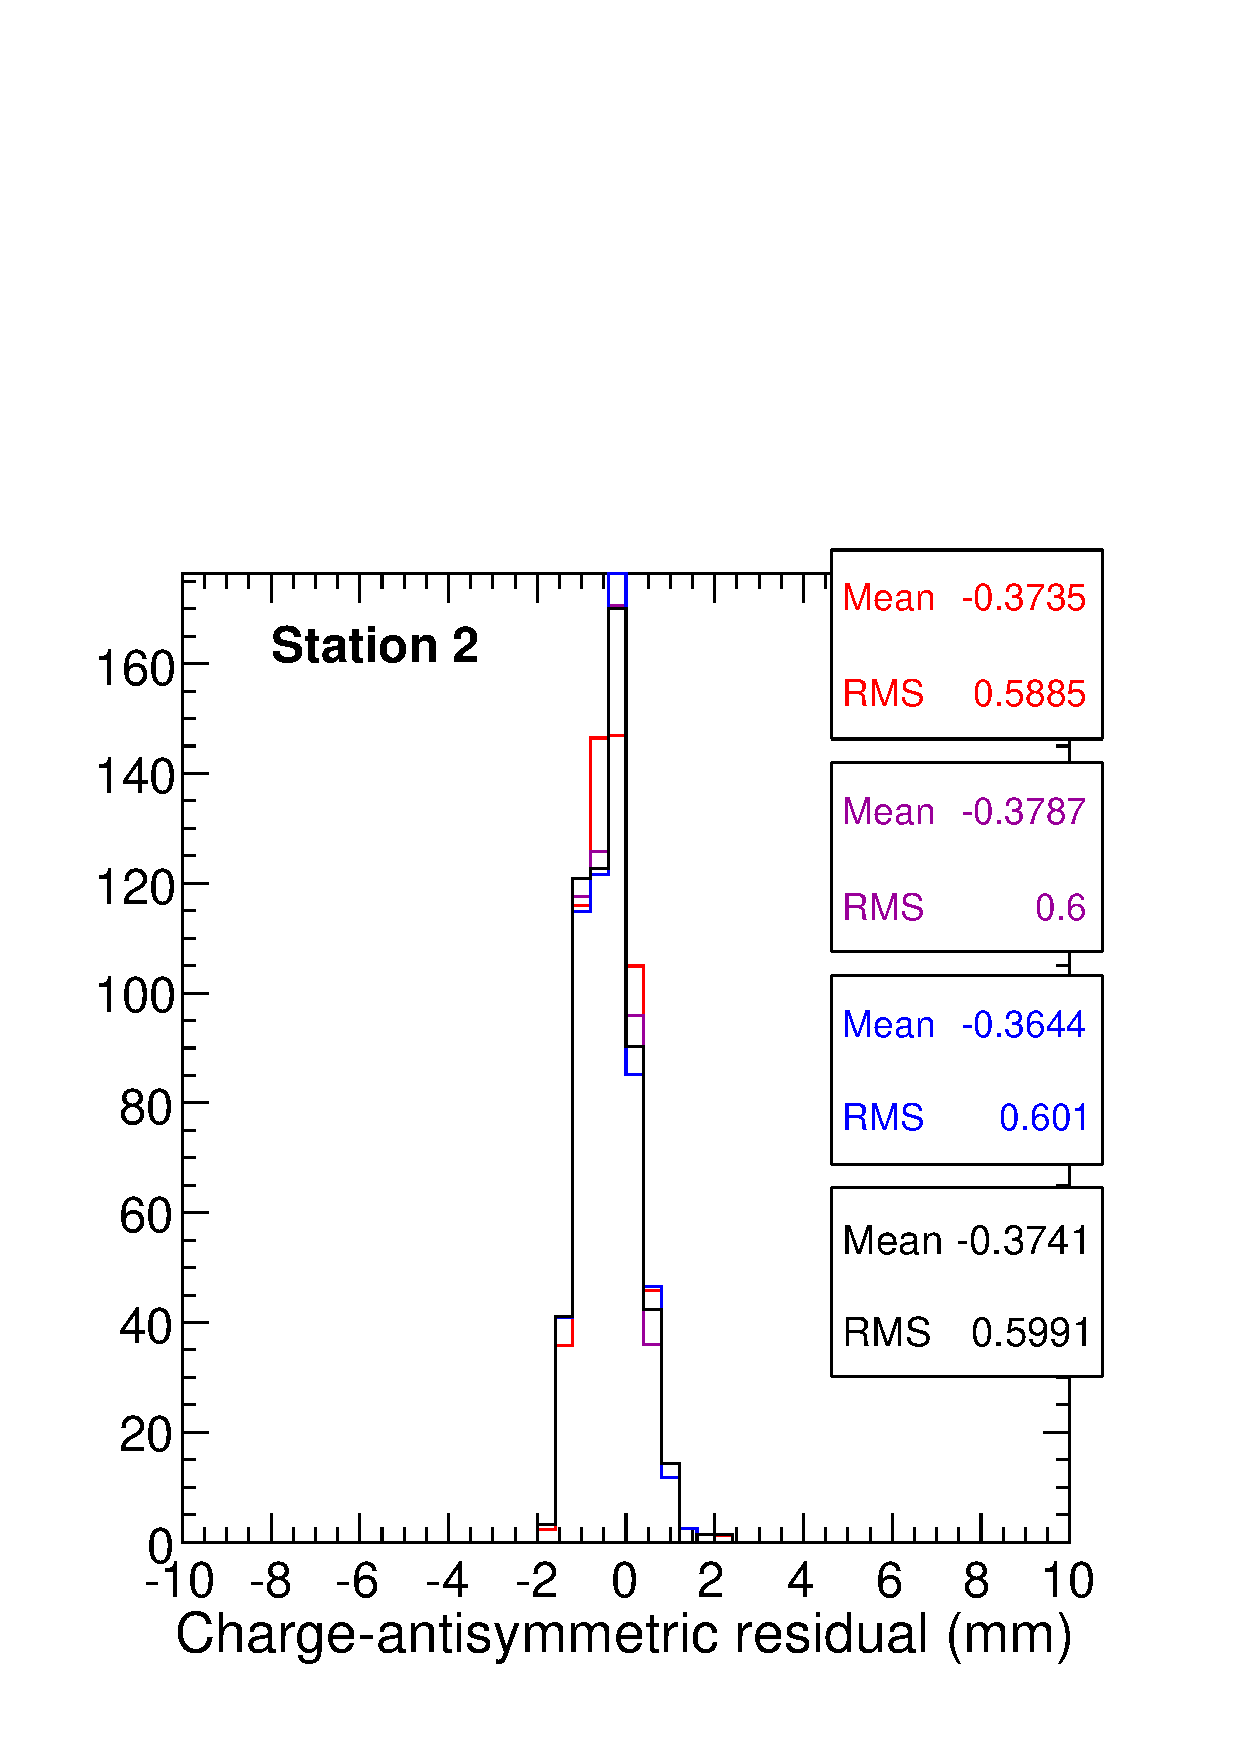
\includegraphics[width=0.5\linewidth]{station2_ptcut90.pdf}

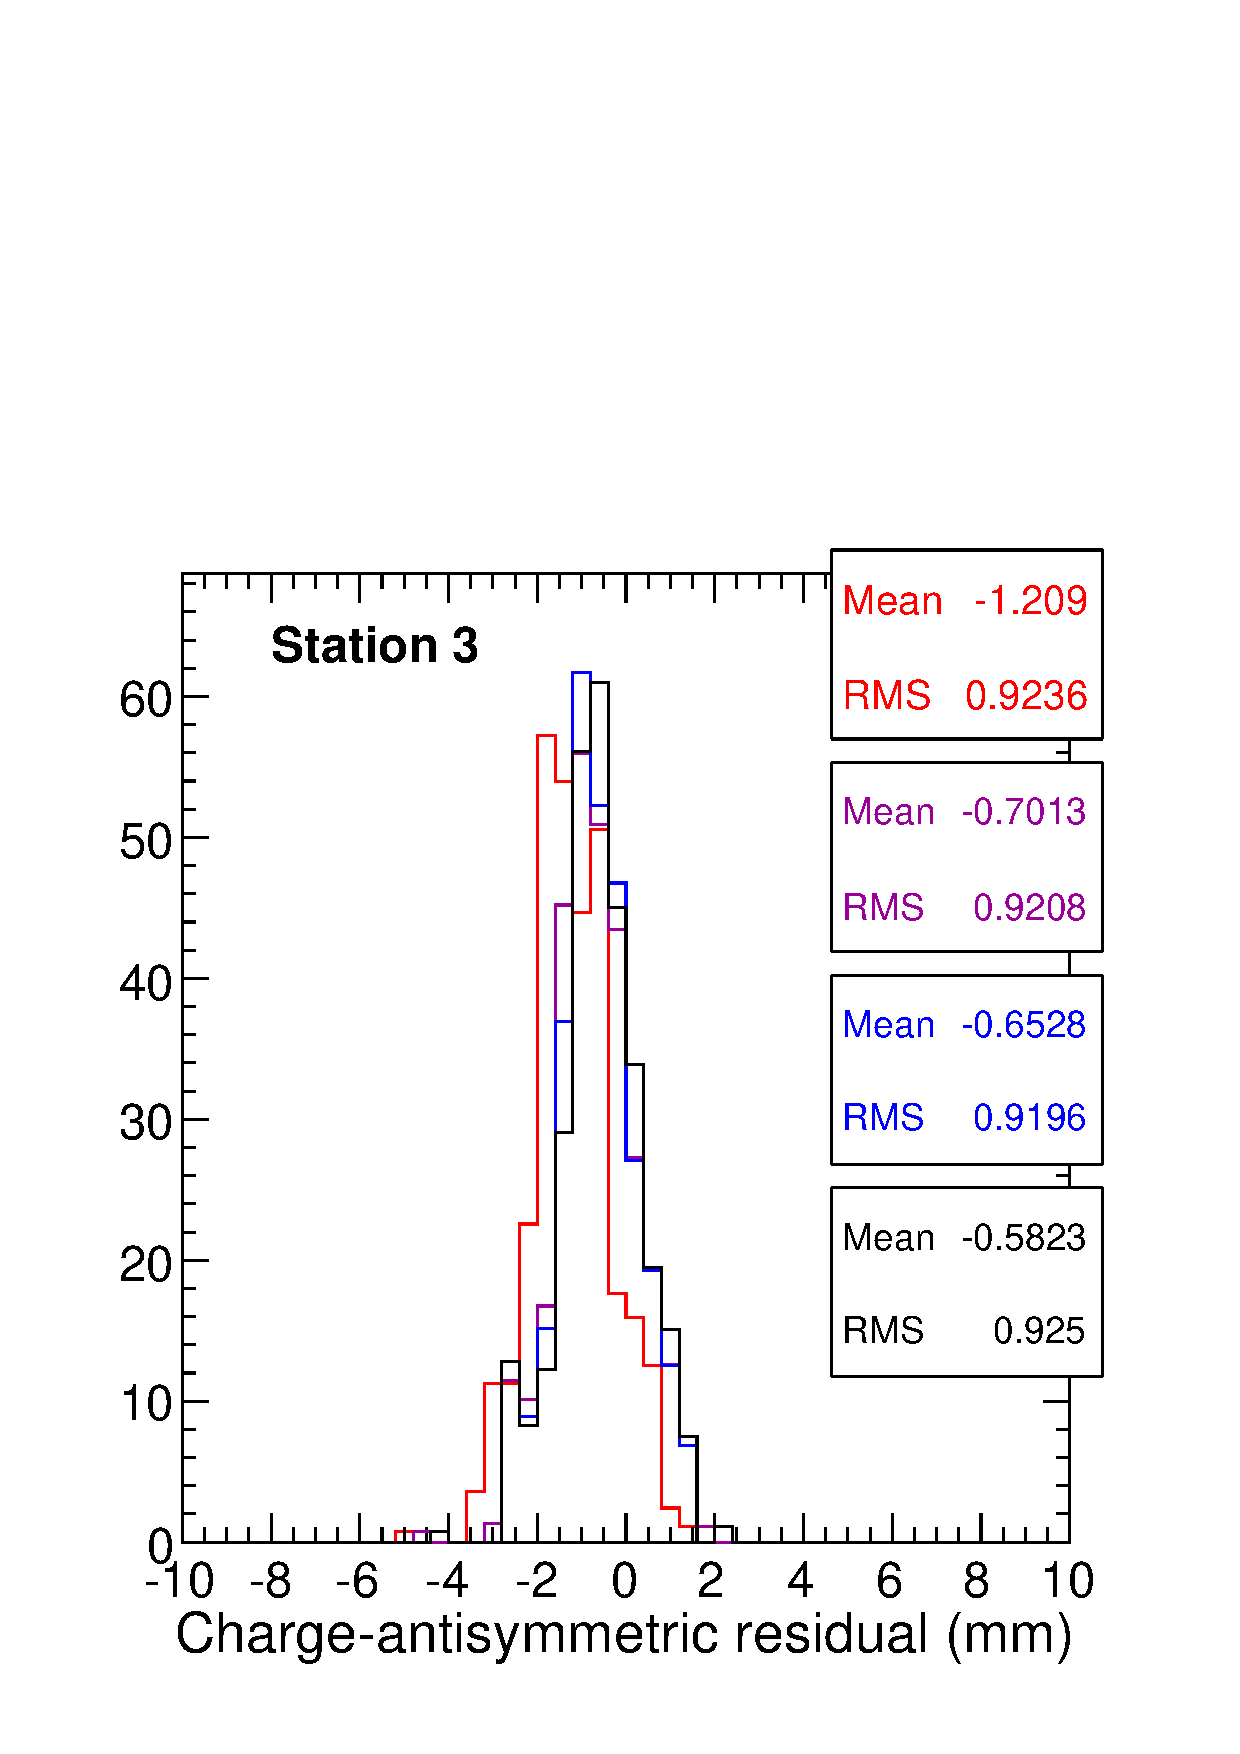
\includegraphics[width=0.5\linewidth]{station3_ptcut90.pdf}
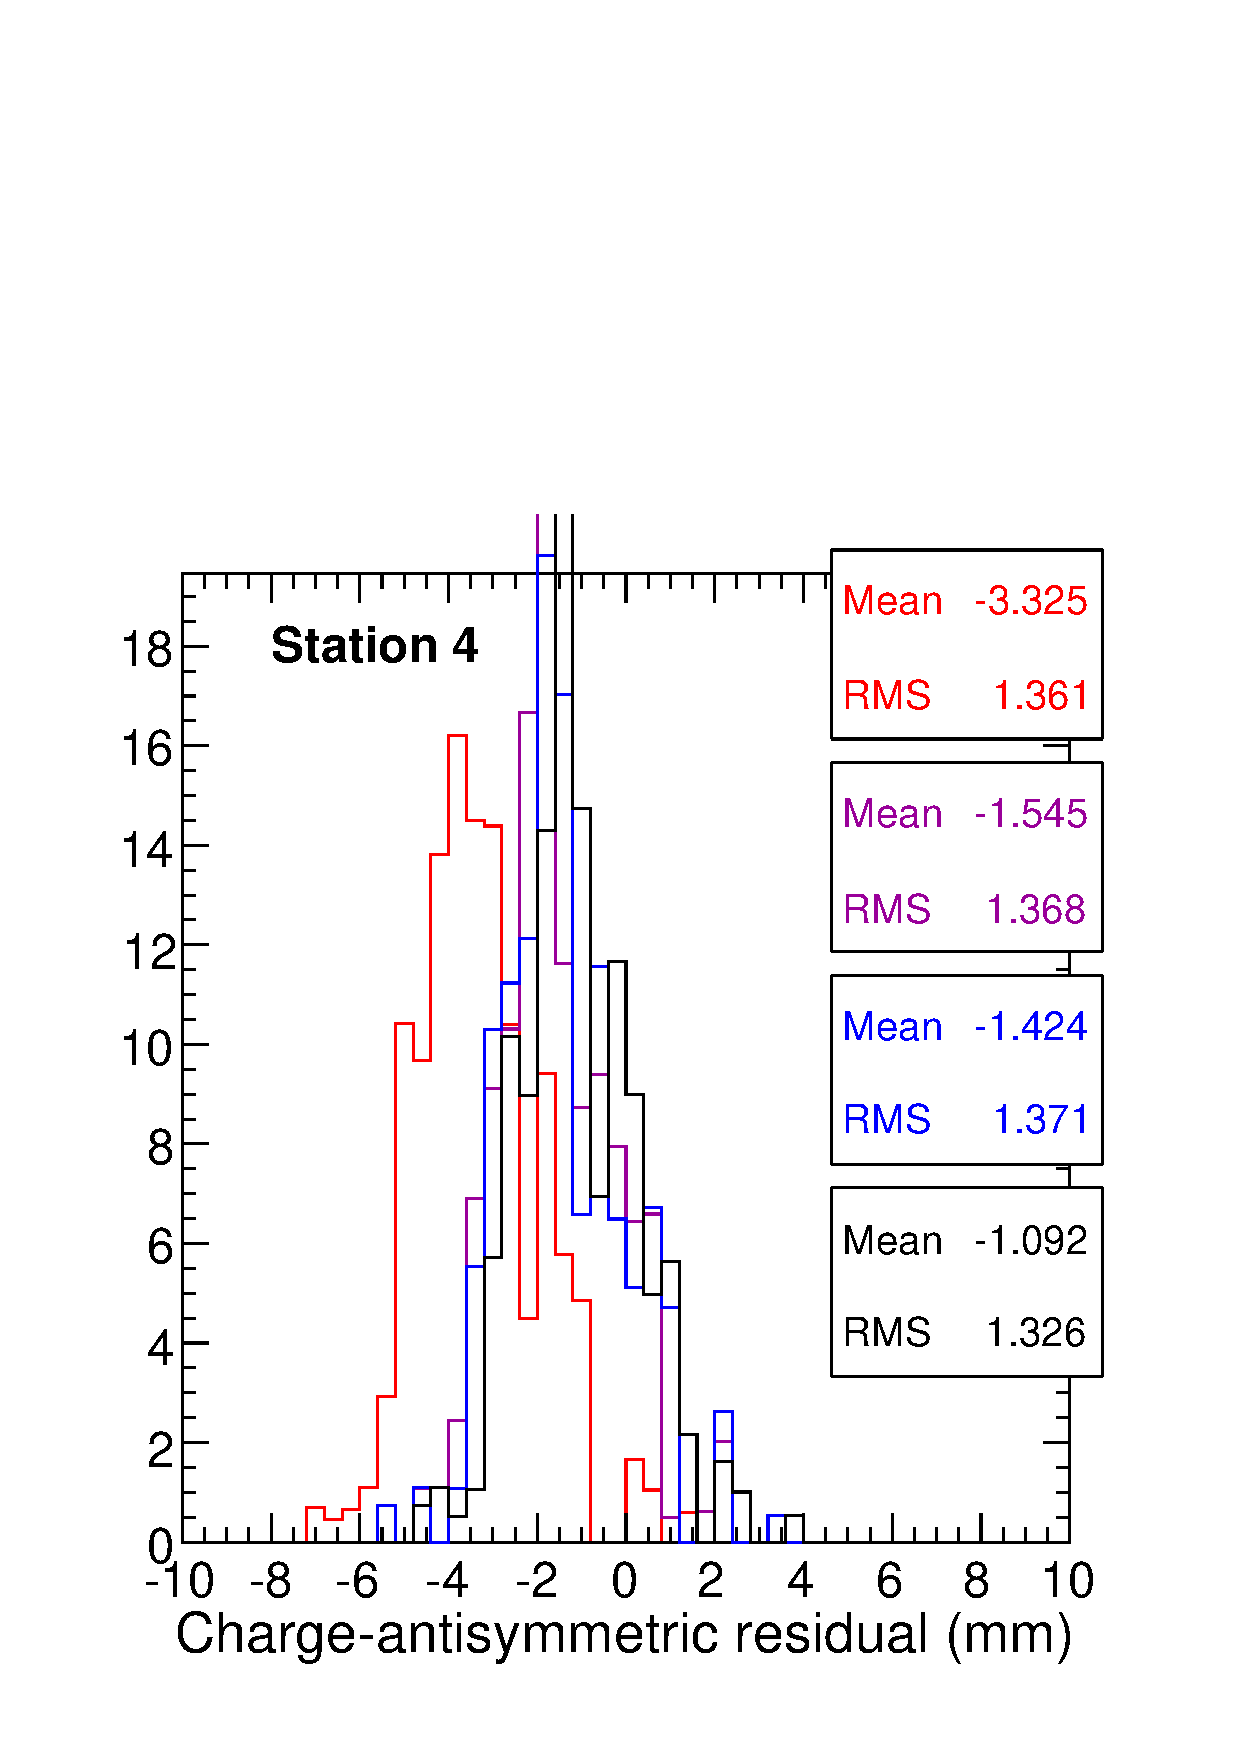
\includegraphics[width=0.5\linewidth]{station4_ptcut90.pdf}

\column{0.3\linewidth}
\scriptsize
\begin{itemize}
\item Same as before, with a higher $p_T$ cut
\item Color code:

\textcolor{red}{red: original map}

\textcolor{purple}{purple: radius $\to$ 30~m}

\textcolor{blue}{blue: radius and $|z|$ $\to$ 30~m}

\textcolor{black}{black: with scaling factors, for 3\_1\_X}

\item Same conclusion: final map not perfectly centered
\end{itemize}
\end{columns}
\end{frame}

\begin{frame}
\frametitle{Results as a function of $p_T$}

\begin{columns}
\column{0.7\linewidth}
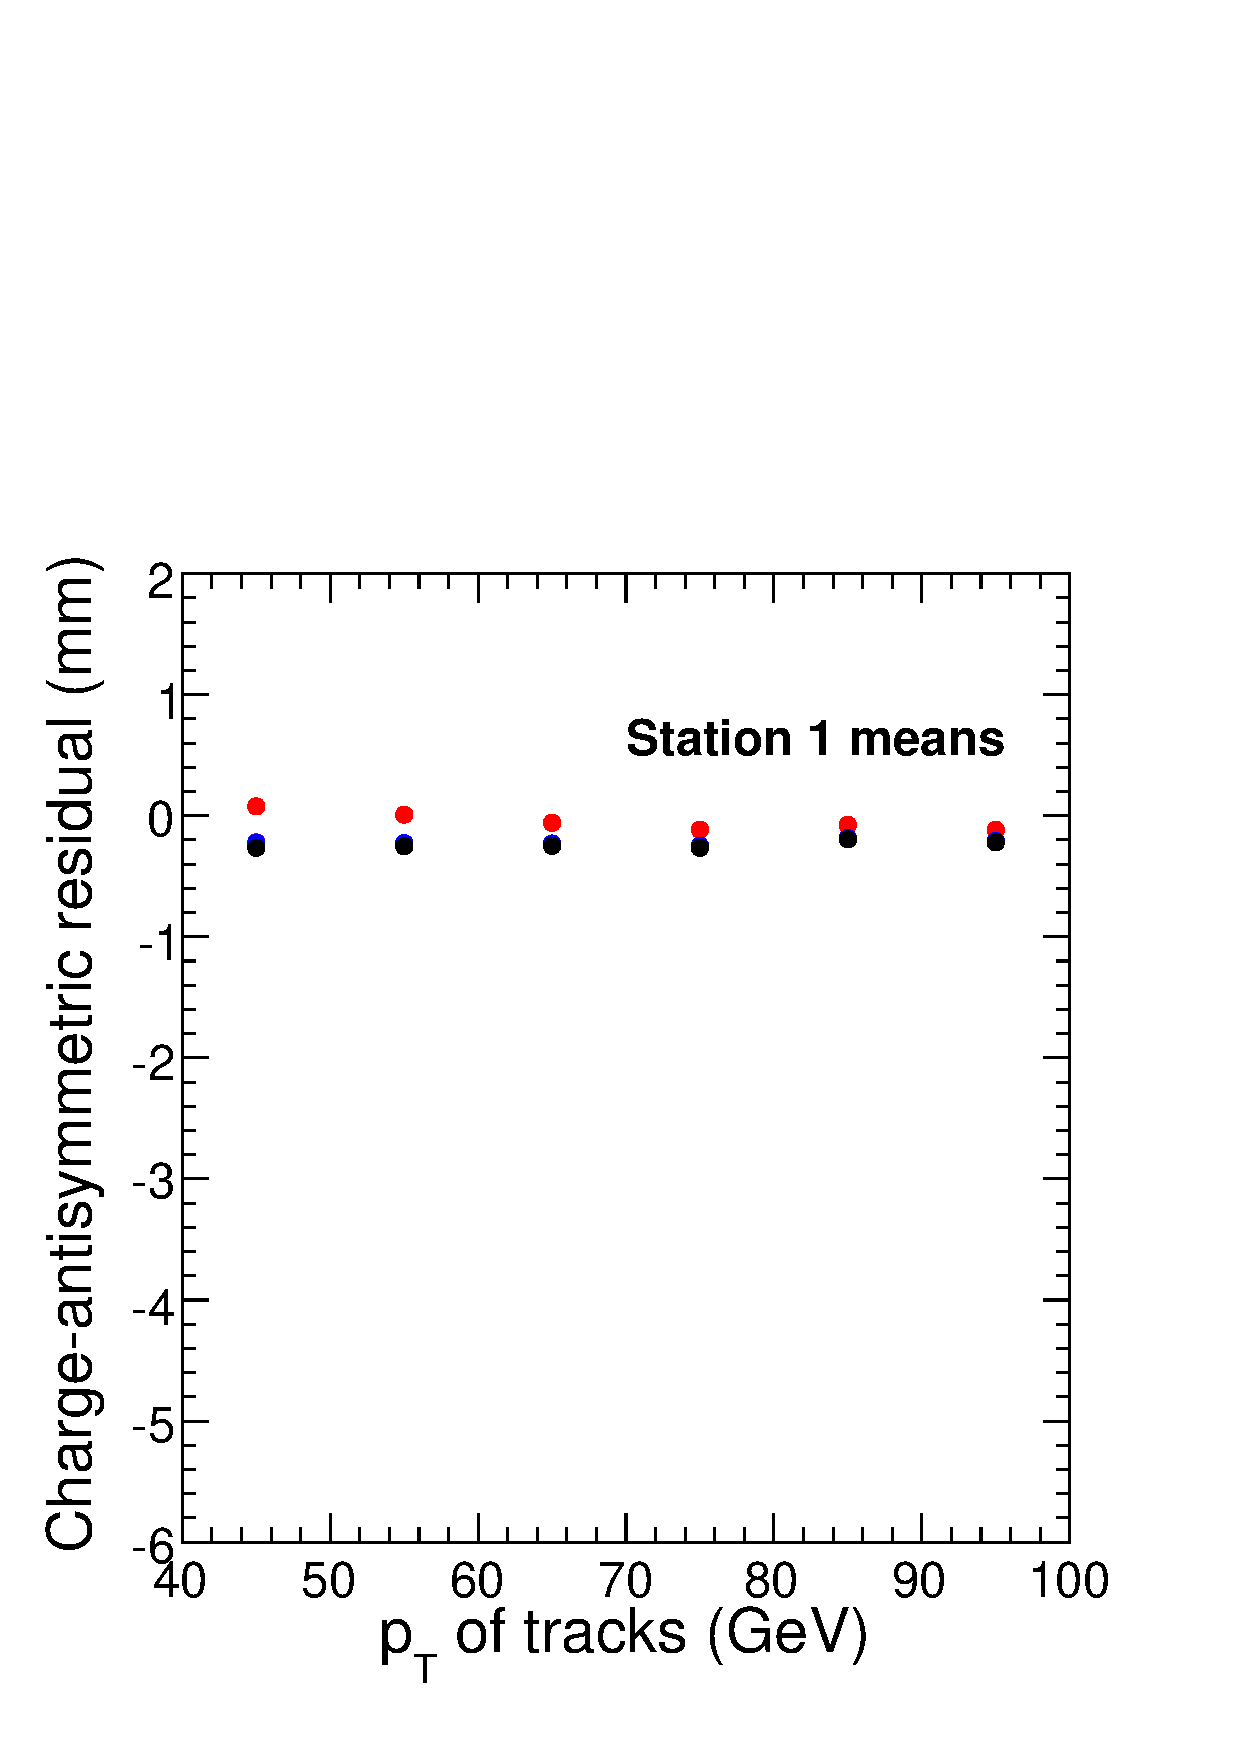
\includegraphics[width=0.5\linewidth]{station1_vspt.pdf}
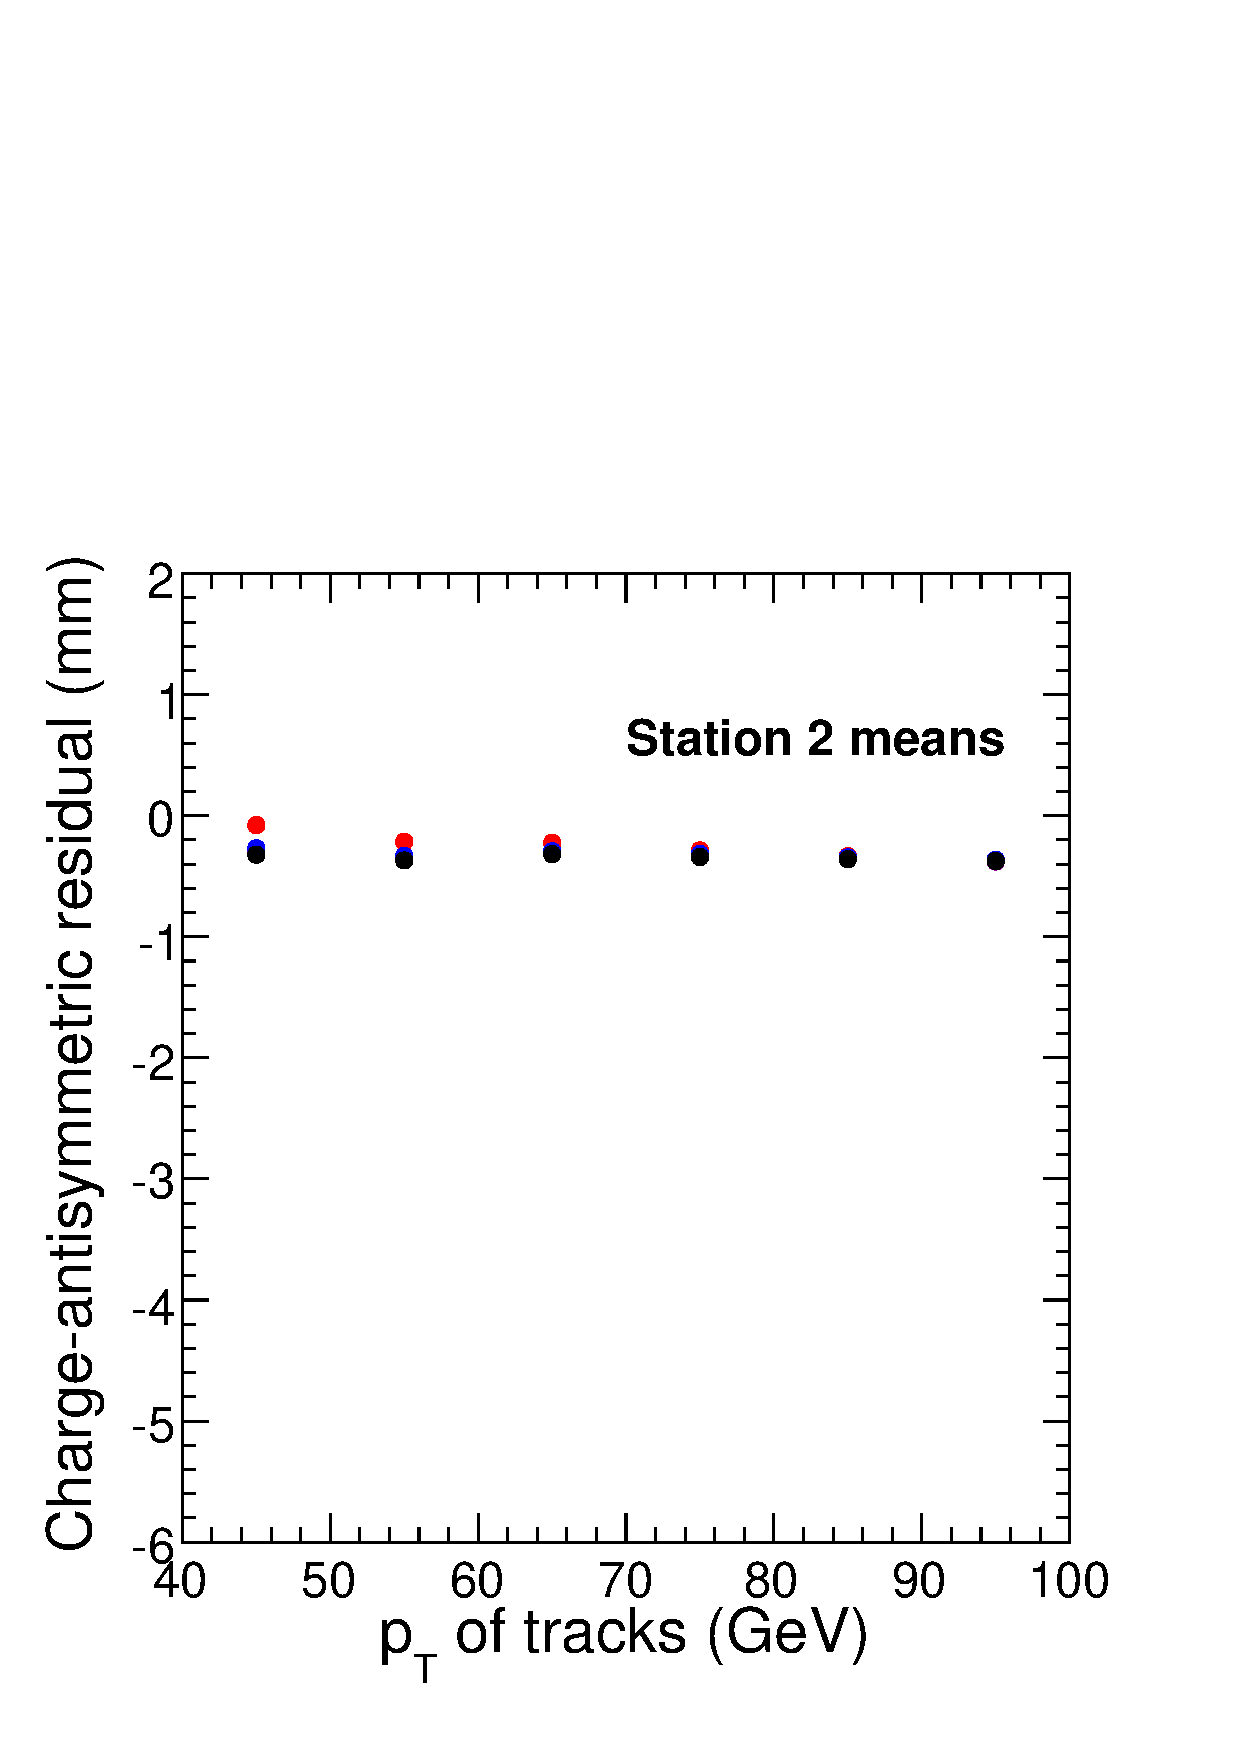
\includegraphics[width=0.5\linewidth]{station2_vspt.pdf}

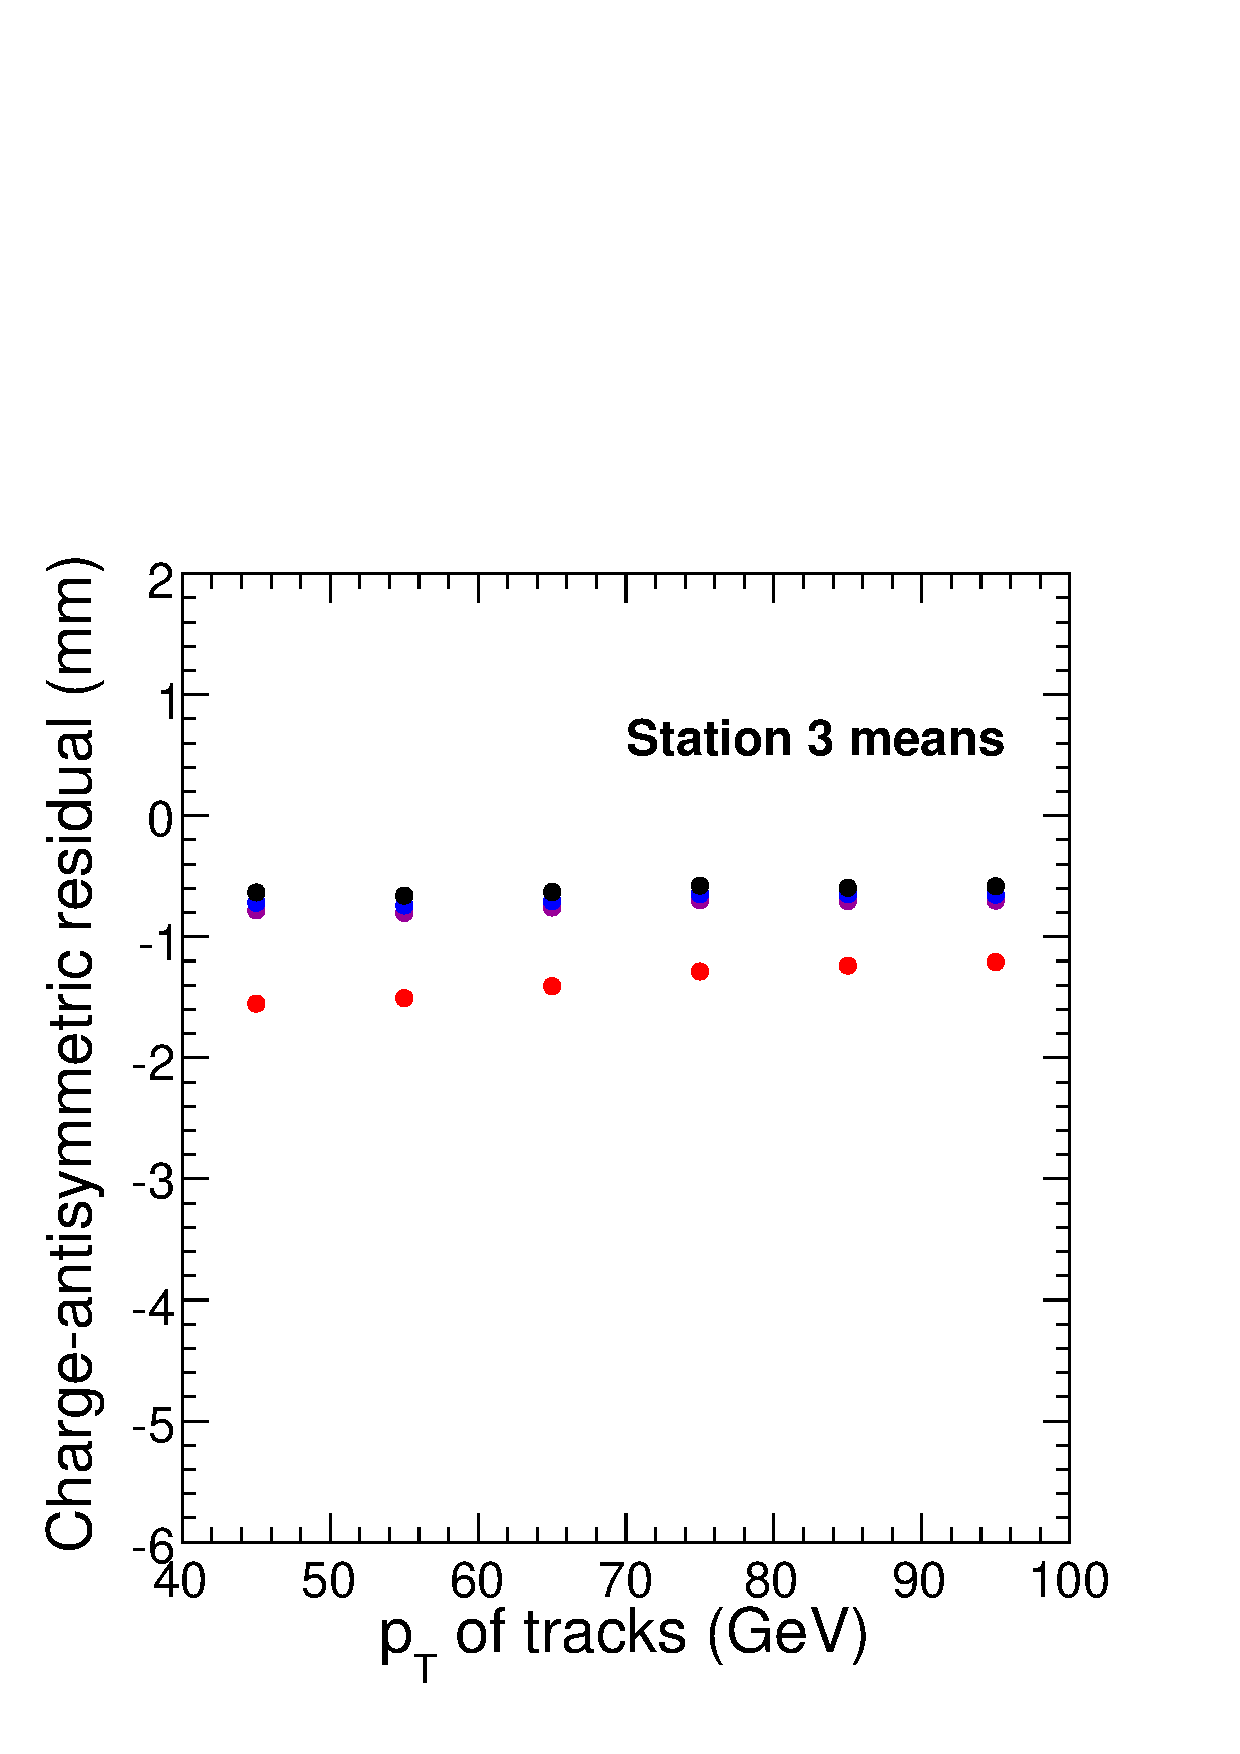
\includegraphics[width=0.5\linewidth]{station3_vspt.pdf}
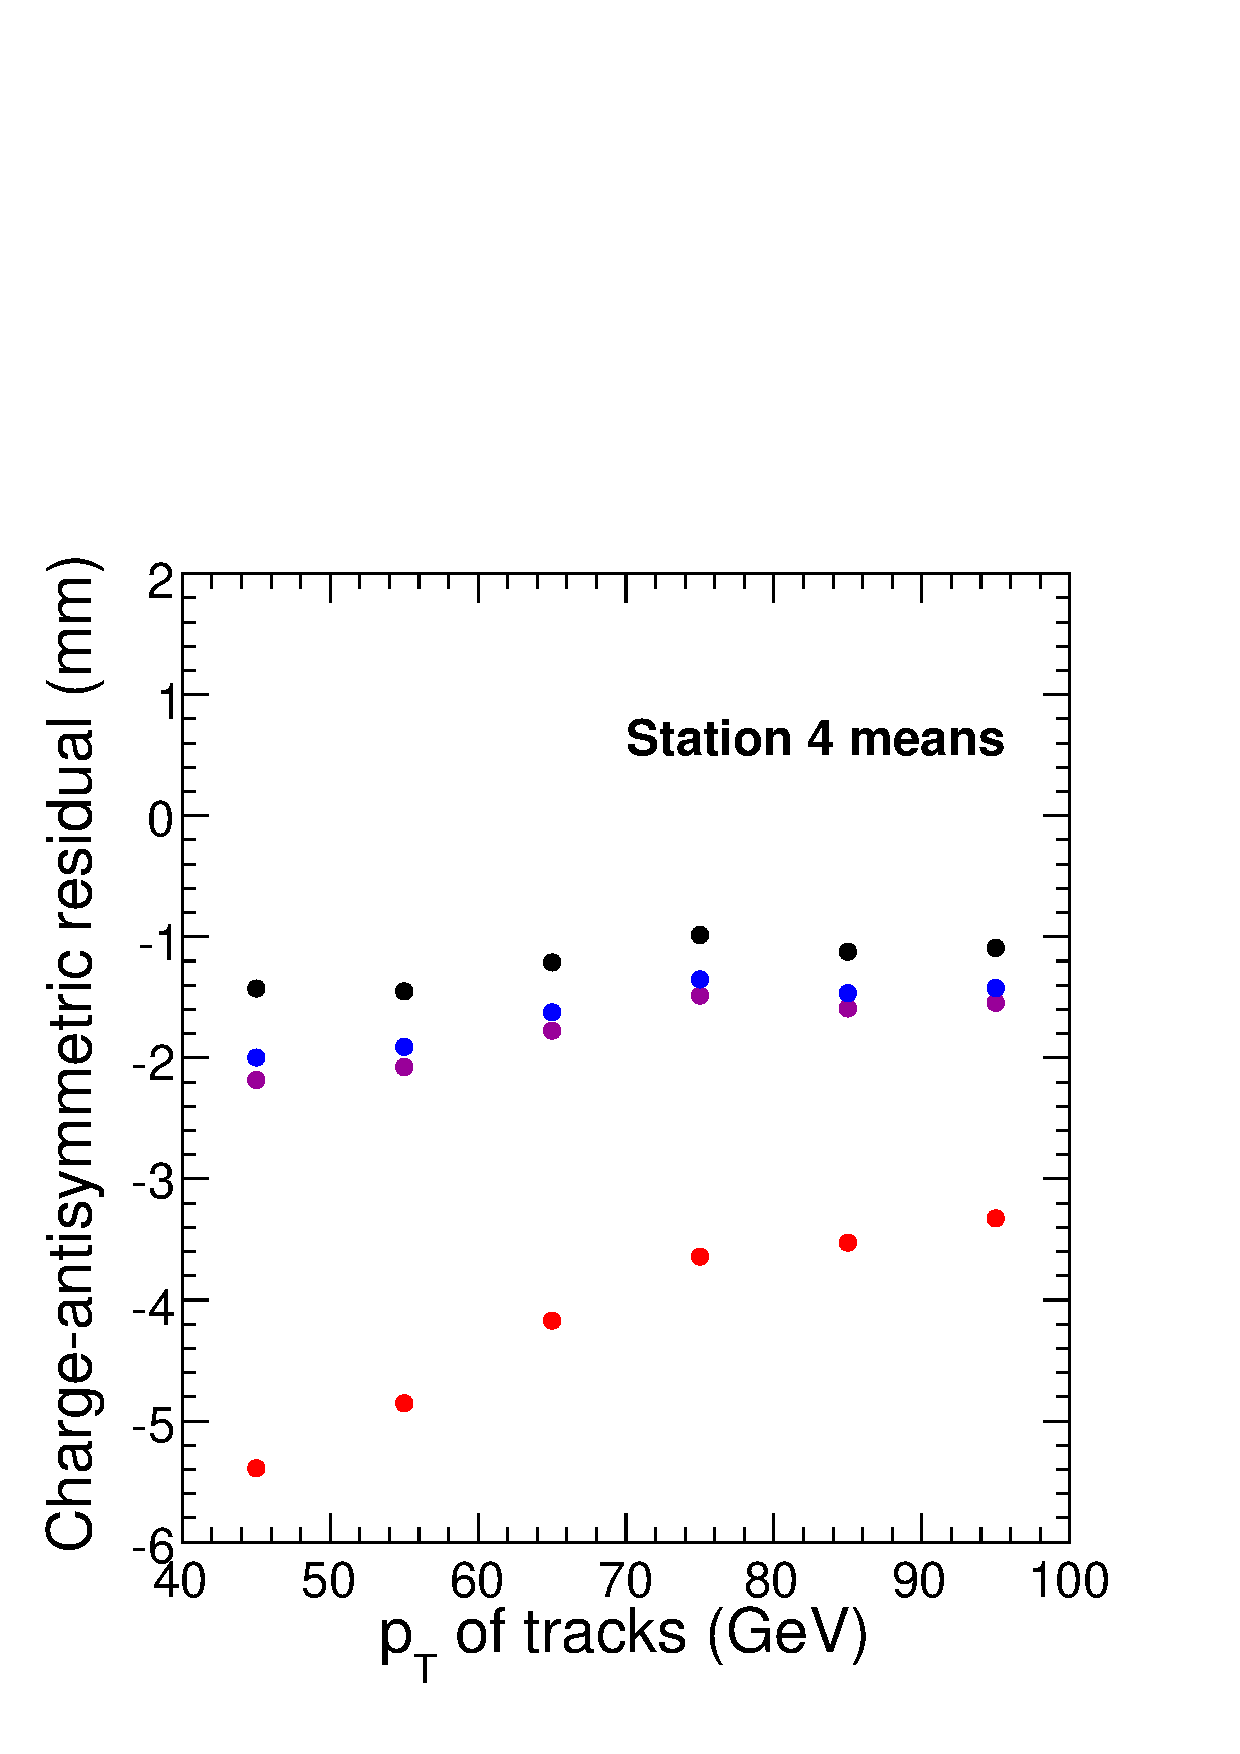
\includegraphics[width=0.5\linewidth]{station4_vspt.pdf}

\column{0.3\linewidth}
\scriptsize
\begin{itemize}
\item Do the same thing in equally-sized $p_T$ bins, plot the mean of each histogram here

\item Color code:

\textcolor{red}{red: original map}

\textcolor{purple}{purple: radius $\to$ 30~m}

\textcolor{blue}{blue: radius and $|z|$ $\to$ 30~m}

\textcolor{black}{black: with scaling factors, for 3\_1\_X}

\item $\vec{B}$-field effects must decrease as $1/p_T$, but after
  \textcolor{red}{original map}, everything's flat!
\item $dE/dx$ falls off faster: $1/{p_T}^2$
\end{itemize}
\end{columns}
\end{frame}

\begin{frame}
\frametitle{Why the constant offset?}

\begin{itemize}
\item Difference between $R_+$ and $R_-$ is 2~mm in station~4, but
  roughly constant with respect to $p_T$
\begin{itemize}
\item independence of $p_T$ rules out the usual suspects: $\vec{B}$ and $dE/dx$
\end{itemize}
\item Charge and entrance angle should be correlated
\item Misalignment in local $z$ can yield opposite position residuals for opposite entrance angles

\begin{center}
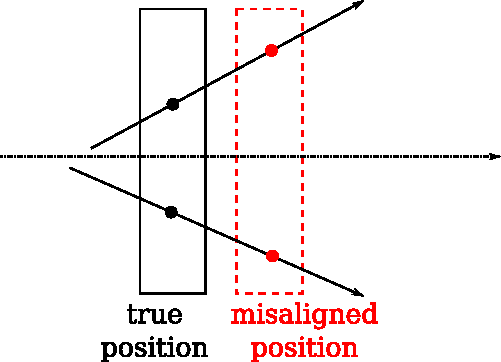
\includegraphics[width=0.35\linewidth]{misalignment_in_z.pdf}
\end{center}

\begin{itemize}
\item local $z$ was corrected for all chambers except station~4
\item local $z$ alignment fit included contributions from $y$ residuals and $y$ entrance angles, as well as $x$ residuals and $x$ entrance angles: in this study, we're only looking at $x$ residuals \mbox{and angles\hspace{-1 cm}}
\end{itemize}
\end{itemize}
\end{frame}

\begin{frame}
\frametitle{Why the constant offset?}

\begin{itemize}
\item Also, ``sawtooth'' effect manifests itself as $x$ residuals versus $x$ entrance angles (but not $y$)
\item So perhaps this is something we've seen before; the new part is that entrance angles are correlated with charges, so the biases vs.~entrance angle become biases wth respect to charge

\end{itemize}

\vfill
\hspace{-0.83 cm} \textcolor{darkblue}{\Large Conclusions}

\vspace{0.25 cm}
\begin{itemize}
\item Charge-antisymmetric residuals are not zero with the latest map
\item But they do not indicate any problems in the magnetic field
\begin{itemize}
\item sensitive to errors in original map, but not any other maps
\end{itemize}
\item We now have some ideas as to what might be wrong \\ (new manifestation of an old problem?)
\end{itemize}
\label{numpages}
\end{frame}


%% \begin{frame}
%% \frametitle{Outline}
%% \begin{itemize}\setlength{\itemsep}{0.75 cm}
%% \item 
%% \end{itemize}
%% \end{frame}

%% \section*{First section}
%% \begin{frame}
%% \begin{center}
%% \Huge \textcolor{blue}{First section}
%% \end{center}
%% \end{frame}

%% \begin{frame}
%% \label{numpages}
%% \end{frame}

\end{document}
